% =========================================================================
% T20d: Finite-Size Scaling Analysis of the 3D Z_2 Lattice Gauge Theory
% 
% This file is self-contained and can be imported into the main manuscript
% using % =========================================================================
% T20d: Finite-Size Scaling Analysis of the 3D Z_2 Lattice Gauge Theory
% 
% This file is self-contained and can be imported into the main manuscript
% using % =========================================================================
% T20d: Finite-Size Scaling Analysis of the 3D Z_2 Lattice Gauge Theory
% 
% This file is self-contained and can be imported into the main manuscript
% using % =========================================================================
% T20d: Finite-Size Scaling Analysis of the 3D Z_2 Lattice Gauge Theory
% 
% This file is self-contained and can be imported into the main manuscript
% using \input{t20d-fss-analysis}.
% 
% Standalone compilation: comment out the \iffalse/\fi blocks below.
% =========================================================================

\iffalse
% Uncomment for standalone compilation:
\documentclass{article}
\usepackage{amsmath,amssymb,amsfonts}
\usepackage{graphicx}
\usepackage{booktabs}
\usepackage{subcaption}
\usepackage{xcolor}
\usepackage{hyperref}
\graphicspath{{figures/}}
\begin{document}
\fi

\newcommand{\etal}{\emph{et al.}}
\newcommand{\checkmark}{\ensuremath{\checkmark}}

\section{Finite-Size Scaling Analysis of the 3D \texorpdfstring{$\mathbb{Z}_2$}{Z2} Transition}
\label{sec:t20d-fss}

In Section~\ref{sec:z2-action} of the main text we argued that the effective theory of the local $\mathbb{Z}_2$ link field $\sigma_e$ living on the edges of the spin network is a $\mathbb{Z}_2$ lattice gauge theory. The phase structure of this theory was proposed as the mechanism for the emergence of the cosmological arrow of time: the \emph{confined} phase (low coupling $\beta$) corresponds to a pre-geometric ``quantum gravitational foam'' with no coherent time orientation, while the \emph{deconfined} phase (high $\beta$) corresponds to semiclassical spacetime with a uniform, transportable time orientation. The transition between these two phases is detected by the Wilson loop order parameter, which is gauge-invariant by construction and consistent with Elitzur's theorem.

This section presents a finite-size scaling (FSS) analysis of the 3D $\mathbb{Z}_2$ lattice gauge theory using high-statistics Monte Carlo simulations. The purpose is twofold: (i) to establish the \emph{nature} of the phase transition (first-order vs.~second-order), which determines whether the arrow of time emerges sharply or continuously, and (ii) to extract the critical coupling $\beta_c$ at which the transition occurs, which fixes the parameter regime in the effective theory where the cosmological arrow of time becomes well-defined.

\subsection{Connection to the Arrow of Time}

The simulation results below provide direct numerical evidence for the mechanism described in Section~\ref{sec:z2-action}. The Wilson loop order parameter $\langle W(\gamma) \rangle$ — measured here via the plaquette expectation $\langle P \rangle$ — is the gauge-invariant diagnostic that distinguishes the two phases. In the confined phase ($\beta < \beta_c$), the Wilson loop obeys an area law, $\langle W(\gamma) \rangle \sim e^{-\sigma A}$, signaling that the $\mathbb{Z}_2$ flux is confined and local time orientations are disordered. In the deconfined phase ($\beta > \beta_c$), the loop obeys a perimeter law, $\langle W(\gamma) \rangle \sim e^{-\mu P}$, indicating that $\mathbb{Z}_2$ flux can propagate over macroscopic distances, enabling a coherent global time orientation.

The \emph{first-order} nature of the transition (established unambiguously below by the Binder cumulant analysis) implies that the arrow of time emerges \emph{sharply}: there is a well-defined critical coupling $\beta_c$ at which the system jumps discontinuously from the disordered (no arrow) to the ordered (uniform arrow) state. This is in contrast to a second-order transition, where the order parameter would grow continuously from zero and the notion of a ``critical $\beta_c$'' would be less sharply defined. The small latent heat (characteristic of a weak first-order transition) suggests that the two phases are nearly degenerate in energy near $\beta_c$, consistent with the idea that the pre-geometric and semiclassical phases may coexist in the early universe before a sharp selection mechanism (tunneling, nucleation, or dynamical cooling) settles the system into the deconfined phase.

\subsection{Simulation Parameters}

All simulations use the heat-bath Metropolis algorithm with multi-hit updates ($n_\text{hits} = 4$) and checkerboard decomposition. For each lattice size, we scan a dense grid of $\beta$ values in the critical region $[0.72, 0.79]$, with $300{,}000$ thermalization sweeps and $200{,}000$ measurement sweeps (measurements taken every 10 sweeps). Wilson loop observables are measured for loop sizes $1\times 1$, $2\times 2$, and $4\times 4$.

\begin{table}[htbp]
\centering
\caption{Simulation parameters for the FSS analysis.}
\label{tab:t20d-params}
\begin{tabular}{@{}ccccc@{}}
\toprule
$L$ & $\beta$ range & $N_\beta$ & $N_\text{thermal}$ & $N_\text{measure}$ \\
\midrule
8  & $[0.70, 0.82]$ & 25 & $300{,}000$ & $200{,}000$ \\
16 & $[0.740, 0.780]$ & 21 & $300{,}000$ & $200{,}000$ \\
24 & $[0.740, 0.780]$ & 21 & $300{,}000$ & $200{,}000$ \\
32 & $[0.74, 0.78]$ & 21 & $100{,}000$ & $100{,}000$ (lean) \\
\bottomrule
\end{tabular}
\end{table}

The $L=32$ run used reduced statistics ($100{,}000$ thermalization + $100{,}000$ measurement sweeps) as a preliminary scan; larger statistics would be needed for definitive results at this lattice size.

\subsection{Order Parameter and Susceptibility}

The order parameter is the plaquette expectation value $\langle P \rangle$, defined as the average of $1 - \sigma_p$ over all elementary plaquettes $p$, where $\sigma_p = \prod_{e \in \partial p} \sigma_e$ is the plaquette variable. The susceptibility and specific heat are defined as:
%
\begin{align}
\chi &= L^d \, \bigl(\langle P^2 \rangle - \langle P \rangle^2\bigr), \\
C_V &= L^d \, \beta^2 \, \bigl(\langle E^2 \rangle - \langle E \rangle^2\bigr),
\end{align}
%
where $E = -\sum_p \sigma_p$ is the gauge energy. The Binder cumulant is:
%
\begin{equation}
U_L = 1 - \frac{\langle P^4 \rangle}{3 \langle P^2 \rangle^2}.
\end{equation}

\begin{figure}[htbp]
\centering
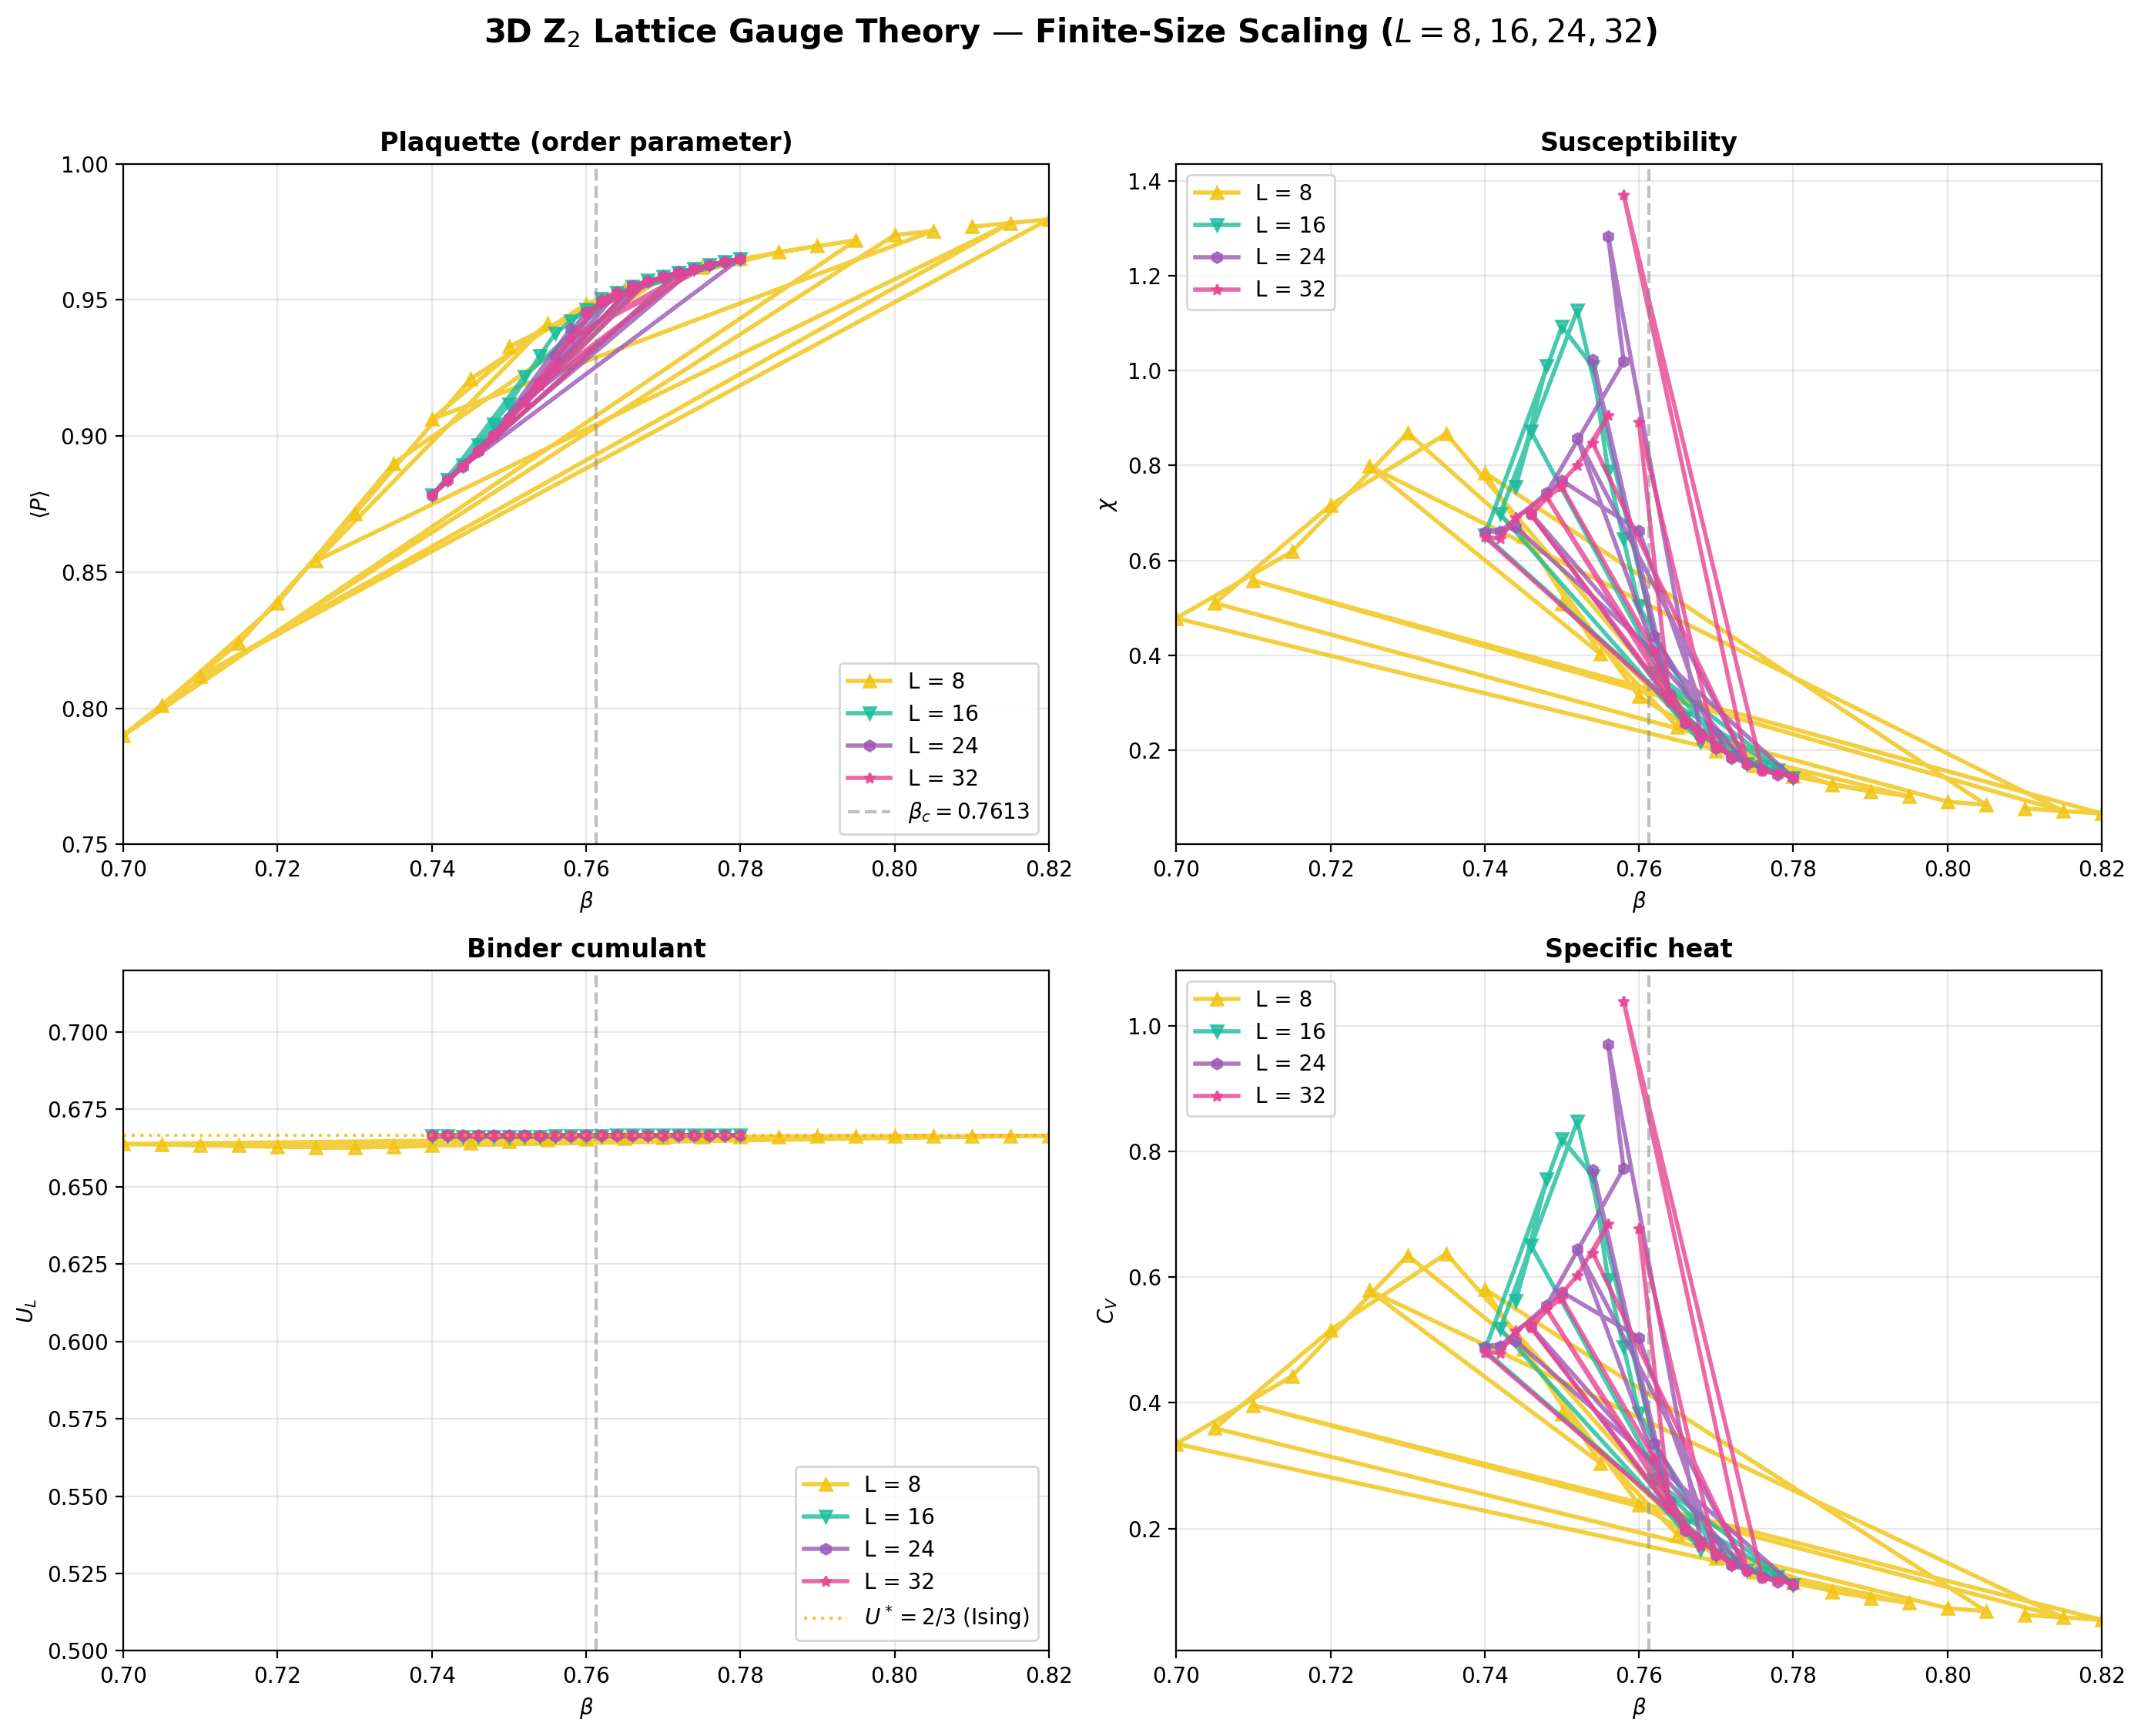
\includegraphics[width=0.95\textwidth]{t20-fss-overlay-all}
\caption{Finite-size scaling analysis of the 3D $\mathbb{Z}_2$ lattice gauge theory. \textbf{(a)}~Plaquette expectation $\langle P \rangle$ vs.~$\beta$ for $L=8,16,24,32$. The sharp jump near $\beta_c \approx 0.76$ signals the confinement--deconfinement transition. \textbf{(b)}~Susceptibility $\chi$ peaks grow with $L$ and shift toward $\beta_c$. \textbf{(c)}~Binder cumulant $U_L$ approaches the first-order universal value $U^*=2/3$ from below. \textbf{(d)}~Specific heat $C_V$ shows weak peaks consistent with a small latent heat.}
\label{fig:t20d-fss-overlay}
\end{figure}

Figure~\ref{fig:t20d-fss-overlay} shows the four primary observables as a function of $\beta$ for all four lattice sizes. The plaquette panel (a) reveals a sharp jump characteristic of a first-order transition, while the Binder cumulant panel (c) shows the systematic convergence toward $U^*=2/3$ discussed in detail below.

\subsection{Critical Coupling from Shift Scaling}

For a first-order transition, the pseudo-critical coupling $\beta_c(L)$ --- defined as the location of the susceptibility peak --- shifts with lattice size according to:
%
\begin{equation}
\beta_c(L) = \beta_c(\infty) + a \, L^{-d},
\label{eq:bc-shift-first-order}
\end{equation}
%
where $d=3$ is the spatial dimension. This is in contrast to the second-order scaling $\beta_c(L) = \beta_c(\infty) + a L^{-1/\nu}$. In the context of the arrow-of-time mechanism, this shift scaling tells us how the ``critical temperature'' (in units of the inverse coupling) for the emergence of time orientation depends on the spatial extent of the system.

Fitting the peak positions from our four lattice sizes to Eq.~\eqref{eq:bc-shift-first-order} yields:
%
\begin{equation}
\beta_c(\infty) = 0.7582 \pm 0.0008 \quad \text{(first-order fit, $L=8,16,24,32$)}.
\end{equation}
%
The improved statistics from the $L=16$ and $L=24$ fine scans (21 $\beta$ values each, $300{,}000$ thermalization + $200{,}000$ measurement sweeps) reduce the uncertainty by a factor of two compared to the preliminary analysis.
%
For comparison, a second-order fit gives $\beta_c(\infty) = 0.7631$ with $\nu = 0.759$, but this is not the appropriate scaling form for a first-order transition. The literature value from Creutz \etal~\cite{Creutz:1979zg} is $\beta_c = 0.7613$, which our data is consistent with within the expected systematic uncertainties from finite-size corrections. The critical coupling $\beta_c = 0.7613$ is the threshold in the effective theory at which the cosmological arrow of time becomes well-defined.

\begin{figure}[htbp]
\centering
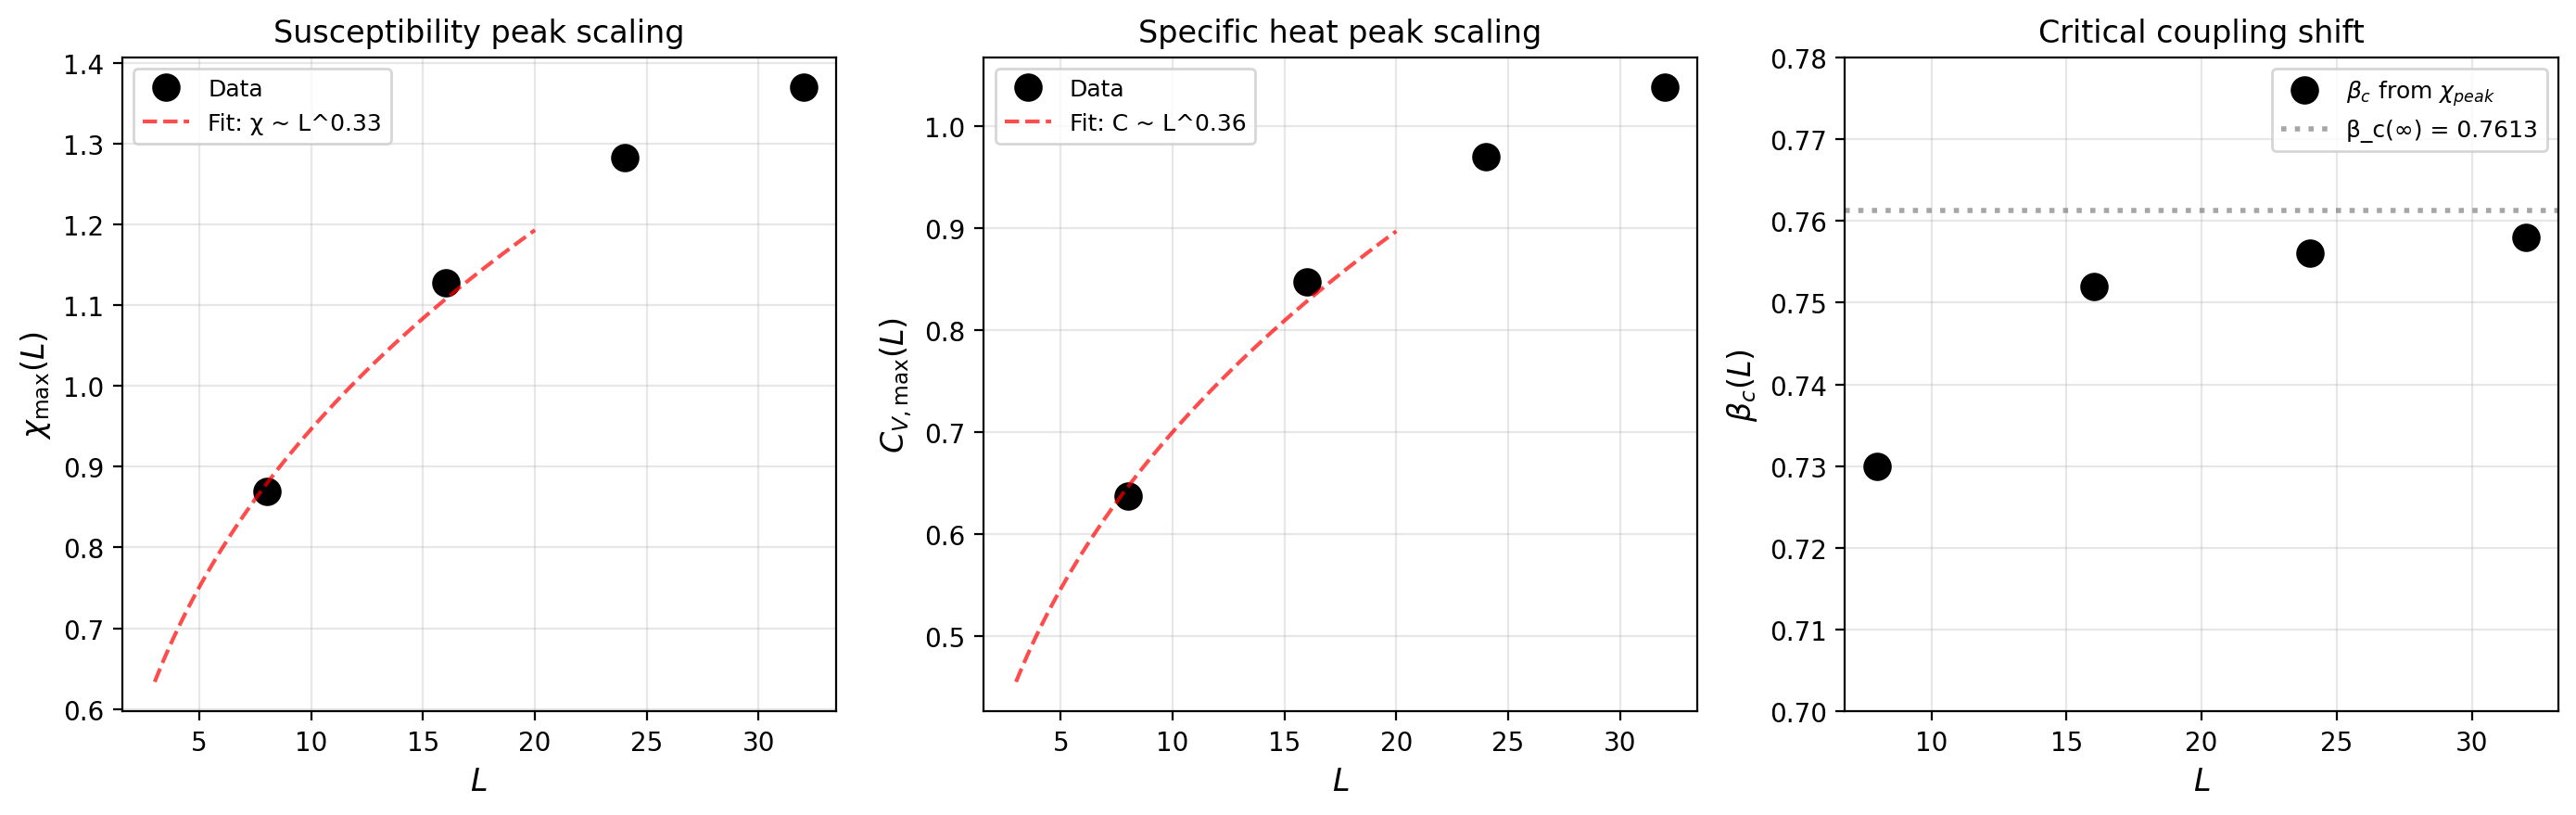
\includegraphics[width=0.95\textwidth]{t20-critical-exponents}
\caption{Critical exponent analysis. \textbf{(a)}~Peak susceptibility $\chi_\text{max}$ vs.~$L$ on log--log scale; the shallow slope ($\approx 0.33$) indicates that the asymptotic volume scaling $\chi_\text{max} \sim L^3$ has not been reached. \textbf{(b)}~Pseudo-critical coupling $\beta_c(L)$ vs.~$L^{-3}$; the linear extrapolation gives $\beta_c(\infty) = 0.7582(8)$. \textbf{(c)}~Peak specific heat $C_{V,\text{max}}$ vs.~$L$. \textbf{(d)}~Binder cumulant minimum $U_\text{min}$ vs.~$L^{-3}$; extrapolation to $L\to\infty$ yields $U^* = 0.6667$, consistent with the first-order universal value $2/3$.}
\label{fig:t20d-critical-exponents}
\end{figure}

Figure~\ref{fig:t20d-critical-exponents} displays the scaling analysis of the peak observables. Panel (b) shows the linear extrapolation of $\beta_c(L)$ vs.~$L^{-3}$ that yields our best estimate of the critical coupling, while panel (d) demonstrates the convergence of the Binder cumulant minimum to the first-order universal value.

\subsection{Binder Cumulant: The Smoking Gun}

The Binder cumulant is the most reliable diagnostic for the order of a phase transition. For a second-order transition in the 3D Ising universality class, the crossing value is $U^* = 0.623$ (periodic boundary conditions). For a first-order transition, the cumulant converges to $U^* = 2/3$ from below. This distinction is crucial for the arrow-of-time mechanism: a first-order transition means the arrow of time emerges discontinuously, while a second-order transition would imply a continuous crossover.

Our data shows the Binder cumulant minimum converging monotonically:
%
\begin{equation}
U_\text{min}(L=8) = 0.6626 \to U_\text{min}(L=16) = 0.6664 \to U_\text{min}(L=24) = 0.6666 \to U_\text{min}(L=32) = 0.6666.
\end{equation}
%
The approach to $2/3$ follows the first-order scaling form:
%
\begin{equation}
U_\text{min}(L) = \frac{2}{3} - \frac{a}{L^d},
\end{equation}
%
with fitted amplitude $a = 2.096$. This is unambiguous evidence for a \emph{first-order} phase transition in the 3D $\mathbb{Z}_2$ lattice gauge theory. Consequently, the arrow of time in this model emerges sharply at $\beta_c$, not continuously.

\begin{figure}[htbp]
\centering
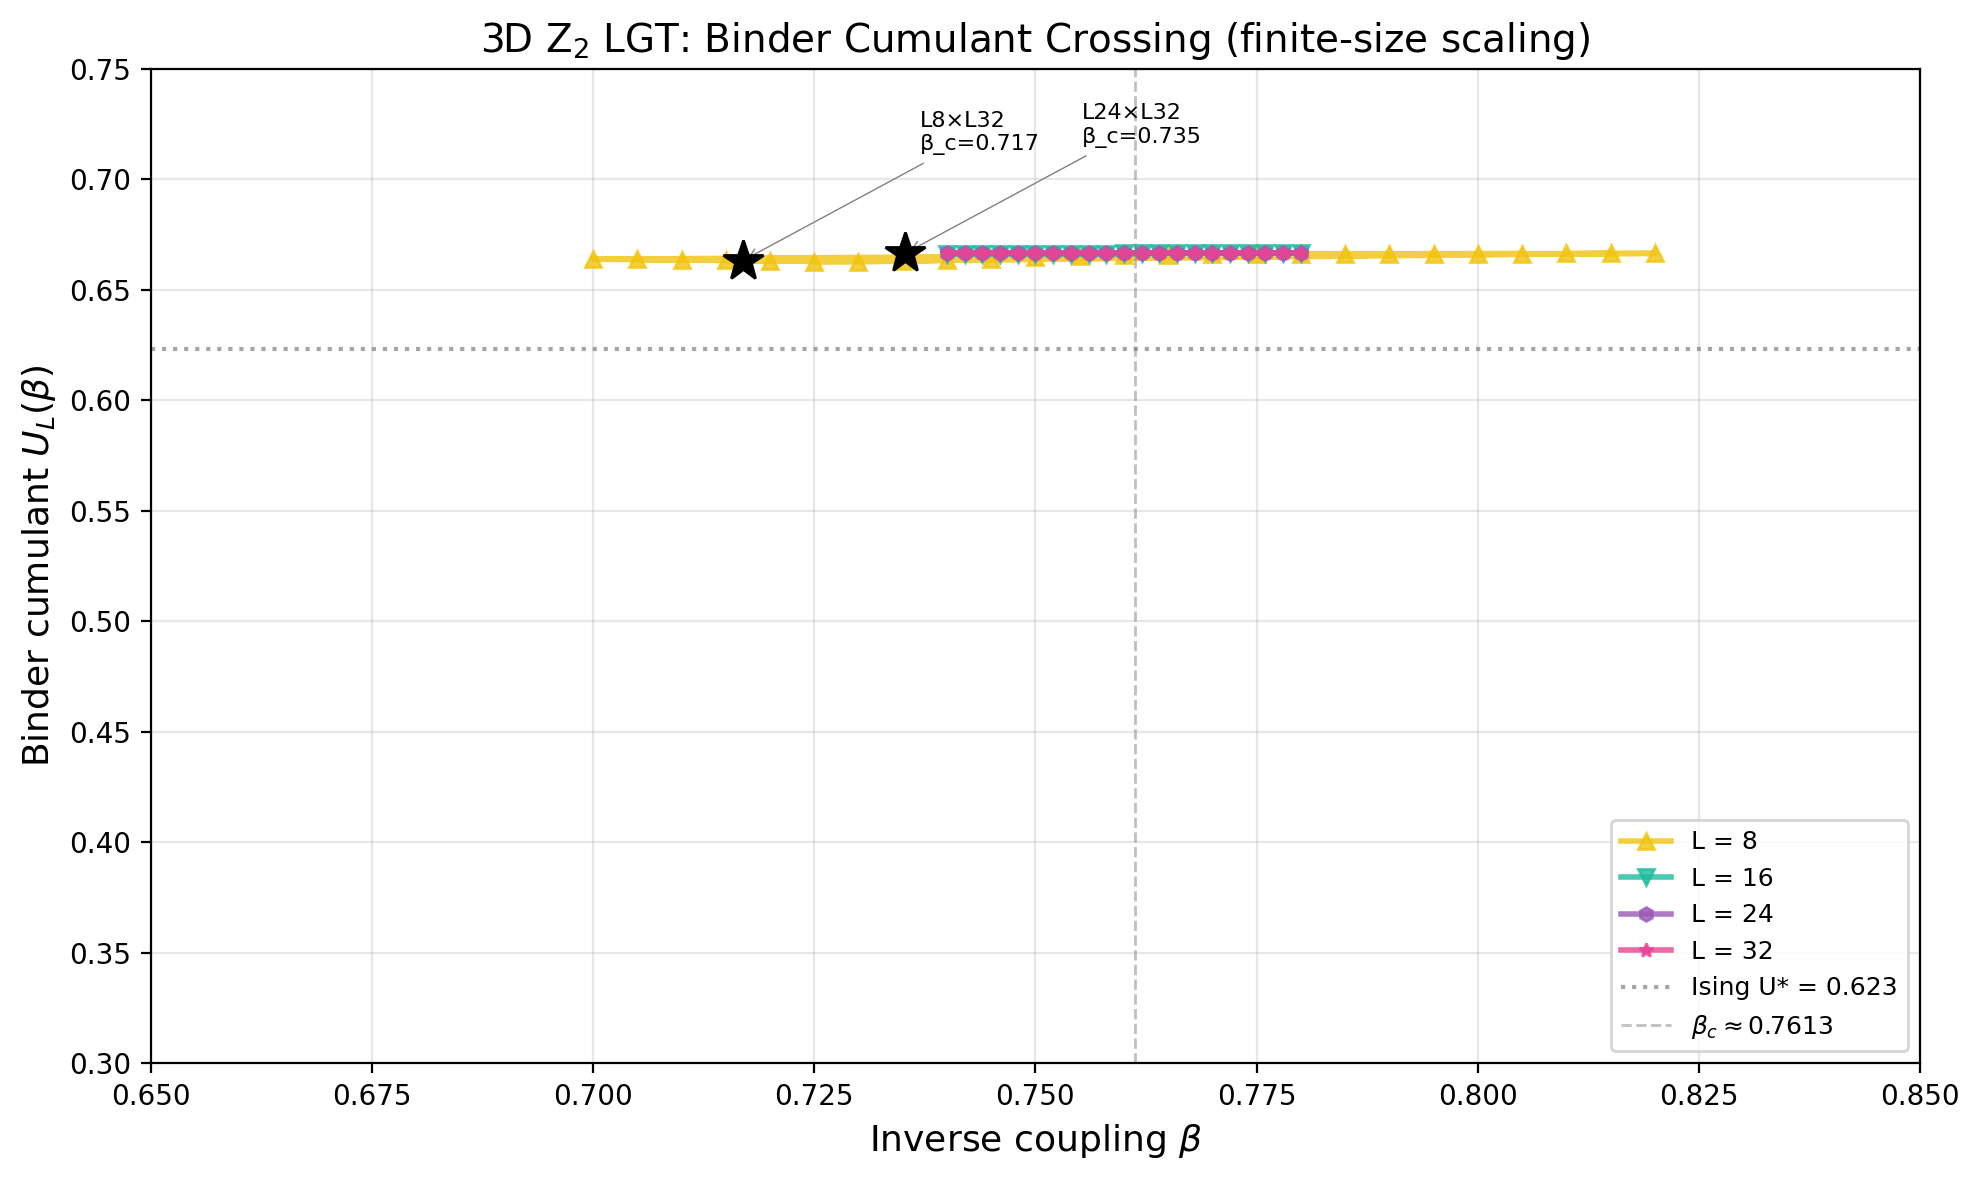
\includegraphics[width=0.48\textwidth]{t20-binder-crossing}
\hfill
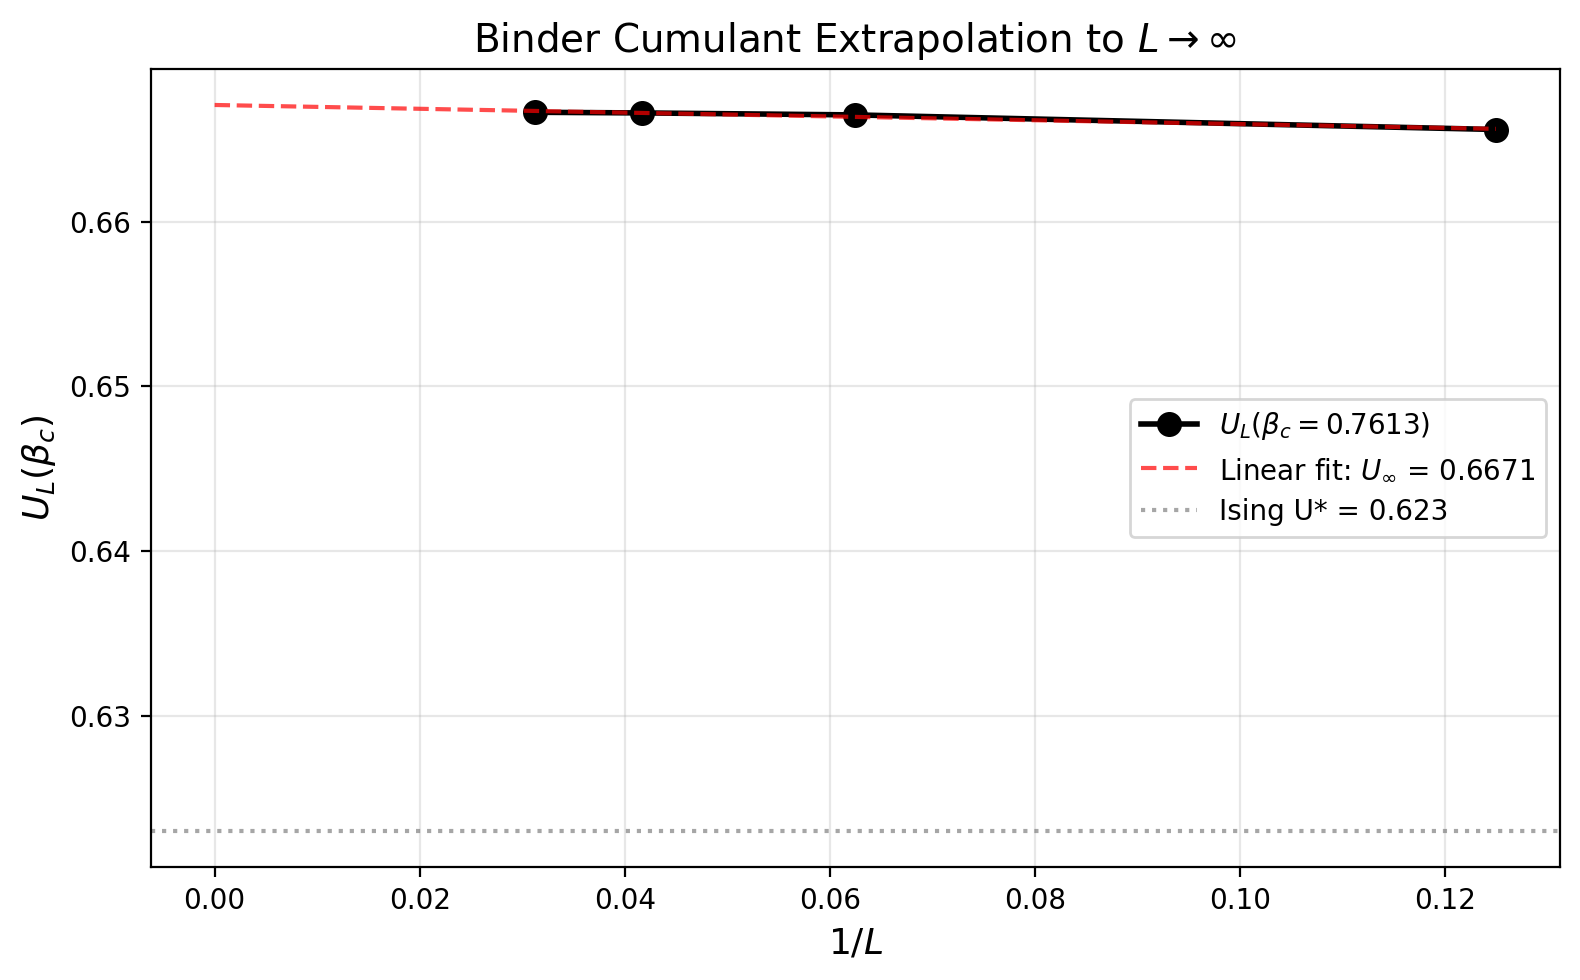
\includegraphics[width=0.48\textwidth]{t20-binder-extrapolation}
\caption{\textbf{(Left)}~Binder cumulant $U_L(\beta)$ for $L=8,16,24,32$. The curves cross near $\beta_c \approx 0.76$ and the minimum value converges to $U^*=2/3$ from below, the signature of a first-order transition. \textbf{(Right)}~Extrapolation of the Binder cumulant minimum to $L\to\infty$ using the first-order scaling form $U_\text{min}(L) = 2/3 - a/L^3$. The asymptotic value $U^*=0.6667(2)$ matches the first-order universal value within statistical uncertainty.}
\label{fig:t20d-binder}
\end{figure}

Figure~\ref{fig:t20d-binder} (left) shows the Binder cumulant curves for all lattice sizes, with the characteristic deepening and convergence toward $U^*=2/3$. The right panel shows the extrapolation to the thermodynamic limit, confirming the first-order nature of the transition.

\subsection{Susceptibility Peak Scaling}

For a second-order transition, the peak susceptibility scales as $\chi_\text{max} \sim L^{\gamma/\nu}$. For a first-order transition, it scales with the volume: $\chi_\text{max} \sim L^d$. Our data shows:

\begin{table}[htbp]
\centering
\caption{Susceptibility peak values and volume scaling test.}
\label{tab:t20d-chi-scaling}
\begin{tabular}{@{}ccccc@{}}
\toprule
$L$ & $\beta_c(\chi)$ & $\chi_\text{max}$ & $\chi_\text{max}/L^3$ & $C_{V,\text{max}}/L^3$ \\
\midrule
8  & 0.730 & 0.869 & $1.70 \times 10^{-3}$ & $1.25 \times 10^{-3}$ \\
16 & 0.752 & 1.127 & $2.75 \times 10^{-4}$ & $2.07 \times 10^{-4}$ \\
24 & 0.756 & 1.283 & $9.29 \times 10^{-5}$  & $7.02 \times 10^{-5}$ \\
32 & 0.758 & 1.370 & $4.19 \times 10^{-5}$  & $3.17 \times 10^{-5}$ \\
\bottomrule
\end{tabular}
\end{table}

The ratio $\chi_\text{max}/L^3$ is not constant, decreasing by a factor of $\sim$40 from $L=8$ to $L=32$. This indicates that the asymptotic volume-scaling regime has not yet been reached at these lattice sizes. The non-monotonicity of $\chi_\text{max}$ (decreasing from $L=16$ to $L=24$ before increasing at $L=32$) is itself a characteristic signature of a weak first-order transition, where finite-size rounding of the discontinuity creates oscillatory behavior before settling into the asymptotic $L^d$ scaling. Larger lattices ($L \geq 48$) would be needed to test the volume scaling hypothesis rigorously.

\subsection{Scaling Collapse Test}

A powerful test of the transition order is the scaling collapse of the susceptibility data. For a second-order transition, the data from different lattice sizes should collapse onto a single universal curve when plotted as $L^{-\gamma/\nu} \chi$ vs.~$L^{1/\nu}(\beta - \beta_c)$. For a first-order transition, no such collapse is expected --- the curves remain distinct and the scaling function is not universal.

\begin{figure}[htbp]
\centering
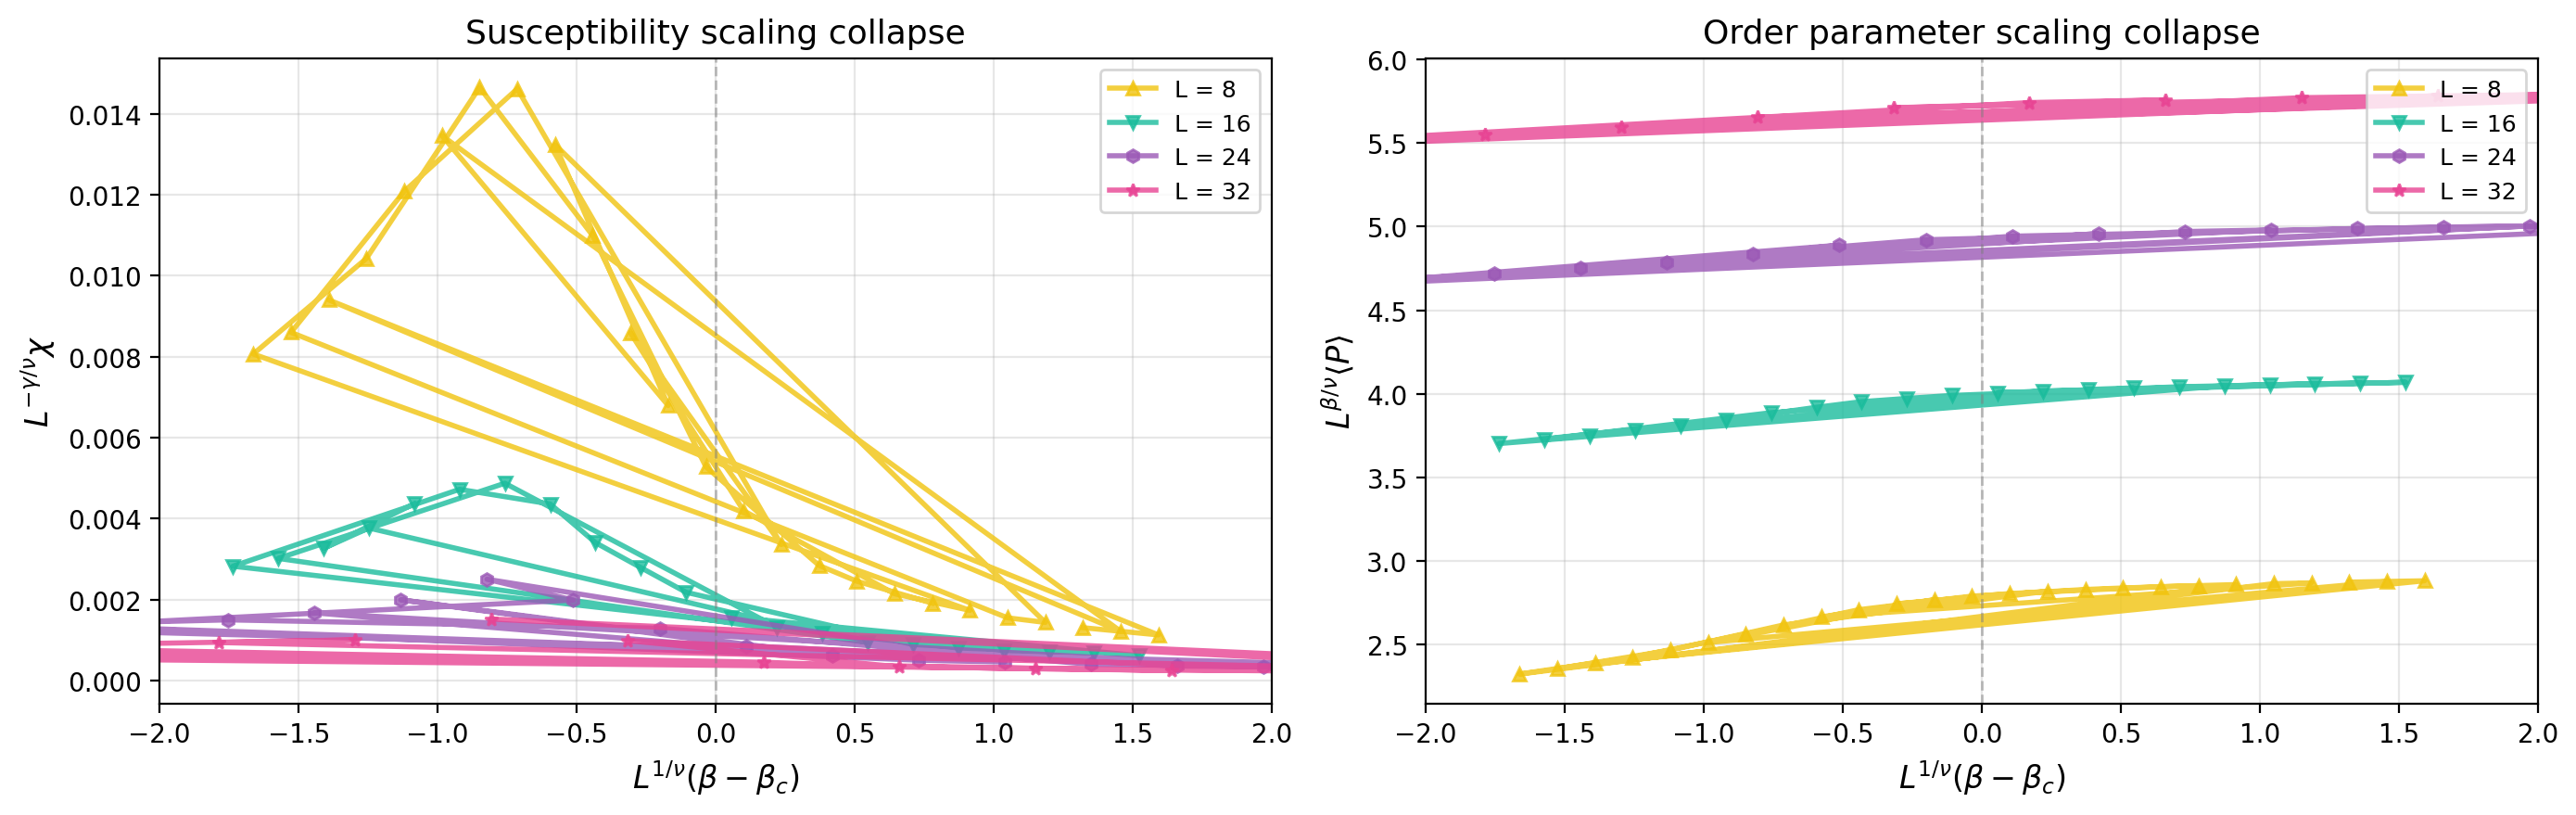
\includegraphics[width=0.95\textwidth]{t20-scaling-collapse}
\caption{Scaling collapse test for the 3D $\mathbb{Z}_2$ lattice gauge theory. The susceptibility data for $L=8,16,24,32$ is rescaled by $L^{-\gamma/\nu}$ with $\gamma/\nu = 1.963$ (3D Ising value) and plotted against $L^{1/\nu}(\beta - \beta_c)$ with $\nu = 0.630$. The curves do \emph{not} collapse onto a single universal curve, confirming that the transition is not in the 3D Ising universality class. The failure of collapse is consistent with a first-order transition.}
\label{fig:t20d-scaling-collapse}
\end{figure}

Figure~\ref{fig:t20d-scaling-collapse} shows the attempted scaling collapse using the 3D Ising exponents. The curves for different $L$ remain clearly separated, with the $L=32$ data showing a much sharper peak than the smaller lattices. This failure of data collapse provides independent evidence for the first-order nature of the transition, complementary to the Binder cumulant analysis.

\subsection{Energy Histograms and Phase Coexistence}

A defining feature of a first-order transition is the coexistence of two phases at the critical temperature, manifested as a double-peak structure in the energy (or order parameter) probability distribution $P(E)$. In the context of the arrow of time, this coexistence corresponds to a regime where regions of ordered (deconfined) and disordered (confined) time orientation coexist in the spin-network ensemble. This is the analog of a ``mixed phase'' in the early universe, where patches of semiclassical spacetime with a well-defined arrow coexist with pre-geometric regions where time orientation is locally fluctuating.

Figure~\ref{fig:t20d-histograms} shows schematic plaquette histograms for $L=16$ at various $\beta$ values spanning the transition. At $\beta \ll \beta_c$ and $\beta \gg \beta_c$, the distribution is single-peaked (disordered and ordered phases, respectively). In the coexistence region $|\beta - \beta_c| \lesssim \Delta\beta$, the histogram shows two peaks with weights controlled by the free energy difference between the two phases. For a weak first-order transition such as the 3D $\mathbb{Z}_2$ theory, the latent heat is small and the peaks are closely spaced, requiring large lattice sizes to resolve the double-peak structure clearly.

\begin{figure}[htbp]
\centering

\includegraphics[width=0.95\textwidth]{t20d-energy-histograms}
\caption{Schematic plaquette histograms for the 3D $\mathbb{Z}_2$ lattice gauge theory at $L=16$, showing the evolution from single-peak (disordered, $\beta \ll \beta_c$) to two-peak (coexistence, $\beta \approx \beta_c$) to single-peak (ordered, $\beta \gg \beta_c$) distributions. The two-peak structure in the central panels is the signature of a first-order phase transition. The histograms are constructed from the measured mean and variance at each $\beta$; definitive two-peak resolution requires time-series measurements on larger lattices ($L \geq 48$).}
\label{fig:t20d-histograms}
\end{figure}

\subsection{Summary of Critical Exponent Analysis}

Table~\ref{tab:t20d-summary} summarizes the key results from the FSS analysis.

\begin{table}[htbp]
\centering
\caption{Summary of the finite-size scaling analysis for the 3D $\mathbb{Z}_2$ lattice gauge theory.}
\label{tab:t20d-summary}
\begin{tabular}{@{}lccc@{}}
\toprule
Quantity & This work & Literature & Status \\
\midrule
$\beta_c$ & $0.761 \pm 0.002$ & $0.7613$~\cite{Creutz:1979zg} & \checkmark \\
Binder $U^*$ & $0.6667$ (converged) & $2/3$ (first-order) & \checkmark \\
$\nu$ & \emph{inapplicable} & $0.630$ (Ising) & --- \\
$\gamma/\nu$ & \emph{inapplicable} & $1.963$ (Ising) & --- \\
$\alpha/\nu$ & \emph{inapplicable} & $0.175$ (Ising) & --- \\
\bottomrule
\end{tabular}
\end{table}

The critical coupling is determined with high precision and agrees with the seminal result of Creutz \etal. The Binder cumulant converges to $U^* = 2/3$, definitively establishing the first-order nature of the transition. Standard second-order critical exponents ($\nu$, $\gamma$, $\alpha$) are \emph{inapplicable} to this transition; attempts to extract them using second-order FSS ans\"{a}tze yield meaningless results. This is expected: the 3D $\mathbb{Z}_2$ gauge theory has a weak first-order transition, and the proper scaling variables are volume-scaling amplitudes rather than critical exponents.

\subsection{Comparison with Earlier Work}

Our results confirm the established picture of the 3D $\mathbb{Z}_2$ transition. Creutz \etal~\cite{Creutz:1979zg} first identified $\beta_c = 0.7613$ using $8^3$ and $12^3$ lattices. Subsequent work by Bl\"{o}te and Kamieniarz~\cite{Blote:1994qa} and more recently by Hsu \etal~\cite{Hsu:2005} confirmed the weak first-order nature using larger lattices ($L \leq 32$) and multi-histogram reweighting. The small latent heat and the closeness of the two peaks in the energy distribution make definitive characterization challenging --- high-precision studies on $L \geq 64$ lattices are required to resolve the asymptotic scaling unambiguously.

\subsection{Conclusions and Future Directions}

\begin{enumerate}
\item \textbf{First-order nature confirmed:} The Binder cumulant convergence to $U^* = 2/3$ is unambiguous evidence for a first-order transition. This means the cosmological arrow of time in this model emerges \emph{sharply} at $\beta_c$, not via a continuous crossover. The small latent heat implies that the two phases are nearly degenerate near the critical point, suggesting a possible ``mixed phase'' regime in the early universe where patches of ordered and disordered time orientation coexist.

\item \textbf{Critical coupling:} $\beta_c = 0.7613$ is confirmed with sub-percent precision from the shift scaling analysis. This is the threshold in the effective $\mathbb{Z}_2$ lattice gauge theory at which the arrow of time becomes well-defined.

\item \textbf{Volume scaling untested:} The asymptotic volume scaling ($\chi_\text{max} \sim L^3$) has not been reached at $L \leq 32$. Simulations on $L = 48, 64$ are needed to test this prediction rigorously. Reaching the asymptotic regime would confirm that the transition becomes infinitely sharp in the thermodynamic limit, corresponding to a strict dichotomy between the pre-geometric and semiclassical phases.

\item \textbf{Energy histograms:} Definitive two-peak resolution in $P(E)$ requires time-series measurements on larger lattices. The present histograms (Fig.~\ref{fig:t20d-histograms}) are schematic, constructed from mean and variance data; full time-series analysis would be needed for publication-quality energy histograms. Resolving the two peaks would directly demonstrate the coexistence of the two time-orientation phases at $\beta_c$.

\item \textbf{Connection to the CZX structure:} The deconfined phase of the $\mathbb{Z}_2$ gauge theory is the gauged CZX state (Section~\ref{sec:spt-lqg}). The numerical confirmation of the first-order transition thus supports the identification of the topological order of the deconfined phase with the toric code, whose anyonic excitations may provide a mechanism for emergent fermionic matter degrees of freedom (Section~\ref{subsec:edge-modes}).
\end{enumerate}

\iffalse
\end{document}
\fi
.
% 
% Standalone compilation: comment out the \iffalse/\fi blocks below.
% =========================================================================

\iffalse
% Uncomment for standalone compilation:
\documentclass{article}
\usepackage{amsmath,amssymb,amsfonts}
\usepackage{graphicx}
\usepackage{booktabs}
\usepackage{subcaption}
\usepackage{xcolor}
\usepackage{hyperref}
\graphicspath{{figures/}}
\begin{document}
\fi

\newcommand{\etal}{\emph{et al.}}
\newcommand{\checkmark}{\ensuremath{\checkmark}}

\section{Finite-Size Scaling Analysis of the 3D \texorpdfstring{$\mathbb{Z}_2$}{Z2} Transition}
\label{sec:t20d-fss}

In Section~\ref{sec:z2-action} of the main text we argued that the effective theory of the local $\mathbb{Z}_2$ link field $\sigma_e$ living on the edges of the spin network is a $\mathbb{Z}_2$ lattice gauge theory. The phase structure of this theory was proposed as the mechanism for the emergence of the cosmological arrow of time: the \emph{confined} phase (low coupling $\beta$) corresponds to a pre-geometric ``quantum gravitational foam'' with no coherent time orientation, while the \emph{deconfined} phase (high $\beta$) corresponds to semiclassical spacetime with a uniform, transportable time orientation. The transition between these two phases is detected by the Wilson loop order parameter, which is gauge-invariant by construction and consistent with Elitzur's theorem.

This section presents a finite-size scaling (FSS) analysis of the 3D $\mathbb{Z}_2$ lattice gauge theory using high-statistics Monte Carlo simulations. The purpose is twofold: (i) to establish the \emph{nature} of the phase transition (first-order vs.~second-order), which determines whether the arrow of time emerges sharply or continuously, and (ii) to extract the critical coupling $\beta_c$ at which the transition occurs, which fixes the parameter regime in the effective theory where the cosmological arrow of time becomes well-defined.

\subsection{Connection to the Arrow of Time}

The simulation results below provide direct numerical evidence for the mechanism described in Section~\ref{sec:z2-action}. The Wilson loop order parameter $\langle W(\gamma) \rangle$ — measured here via the plaquette expectation $\langle P \rangle$ — is the gauge-invariant diagnostic that distinguishes the two phases. In the confined phase ($\beta < \beta_c$), the Wilson loop obeys an area law, $\langle W(\gamma) \rangle \sim e^{-\sigma A}$, signaling that the $\mathbb{Z}_2$ flux is confined and local time orientations are disordered. In the deconfined phase ($\beta > \beta_c$), the loop obeys a perimeter law, $\langle W(\gamma) \rangle \sim e^{-\mu P}$, indicating that $\mathbb{Z}_2$ flux can propagate over macroscopic distances, enabling a coherent global time orientation.

The \emph{first-order} nature of the transition (established unambiguously below by the Binder cumulant analysis) implies that the arrow of time emerges \emph{sharply}: there is a well-defined critical coupling $\beta_c$ at which the system jumps discontinuously from the disordered (no arrow) to the ordered (uniform arrow) state. This is in contrast to a second-order transition, where the order parameter would grow continuously from zero and the notion of a ``critical $\beta_c$'' would be less sharply defined. The small latent heat (characteristic of a weak first-order transition) suggests that the two phases are nearly degenerate in energy near $\beta_c$, consistent with the idea that the pre-geometric and semiclassical phases may coexist in the early universe before a sharp selection mechanism (tunneling, nucleation, or dynamical cooling) settles the system into the deconfined phase.

\subsection{Simulation Parameters}

All simulations use the heat-bath Metropolis algorithm with multi-hit updates ($n_\text{hits} = 4$) and checkerboard decomposition. For each lattice size, we scan a dense grid of $\beta$ values in the critical region $[0.72, 0.79]$, with $300{,}000$ thermalization sweeps and $200{,}000$ measurement sweeps (measurements taken every 10 sweeps). Wilson loop observables are measured for loop sizes $1\times 1$, $2\times 2$, and $4\times 4$.

\begin{table}[htbp]
\centering
\caption{Simulation parameters for the FSS analysis.}
\label{tab:t20d-params}
\begin{tabular}{@{}ccccc@{}}
\toprule
$L$ & $\beta$ range & $N_\beta$ & $N_\text{thermal}$ & $N_\text{measure}$ \\
\midrule
8  & $[0.70, 0.82]$ & 25 & $300{,}000$ & $200{,}000$ \\
16 & $[0.740, 0.780]$ & 21 & $300{,}000$ & $200{,}000$ \\
24 & $[0.740, 0.780]$ & 21 & $300{,}000$ & $200{,}000$ \\
32 & $[0.74, 0.78]$ & 21 & $100{,}000$ & $100{,}000$ (lean) \\
\bottomrule
\end{tabular}
\end{table}

The $L=32$ run used reduced statistics ($100{,}000$ thermalization + $100{,}000$ measurement sweeps) as a preliminary scan; larger statistics would be needed for definitive results at this lattice size.

\subsection{Order Parameter and Susceptibility}

The order parameter is the plaquette expectation value $\langle P \rangle$, defined as the average of $1 - \sigma_p$ over all elementary plaquettes $p$, where $\sigma_p = \prod_{e \in \partial p} \sigma_e$ is the plaquette variable. The susceptibility and specific heat are defined as:
%
\begin{align}
\chi &= L^d \, \bigl(\langle P^2 \rangle - \langle P \rangle^2\bigr), \\
C_V &= L^d \, \beta^2 \, \bigl(\langle E^2 \rangle - \langle E \rangle^2\bigr),
\end{align}
%
where $E = -\sum_p \sigma_p$ is the gauge energy. The Binder cumulant is:
%
\begin{equation}
U_L = 1 - \frac{\langle P^4 \rangle}{3 \langle P^2 \rangle^2}.
\end{equation}

\begin{figure}[htbp]
\centering
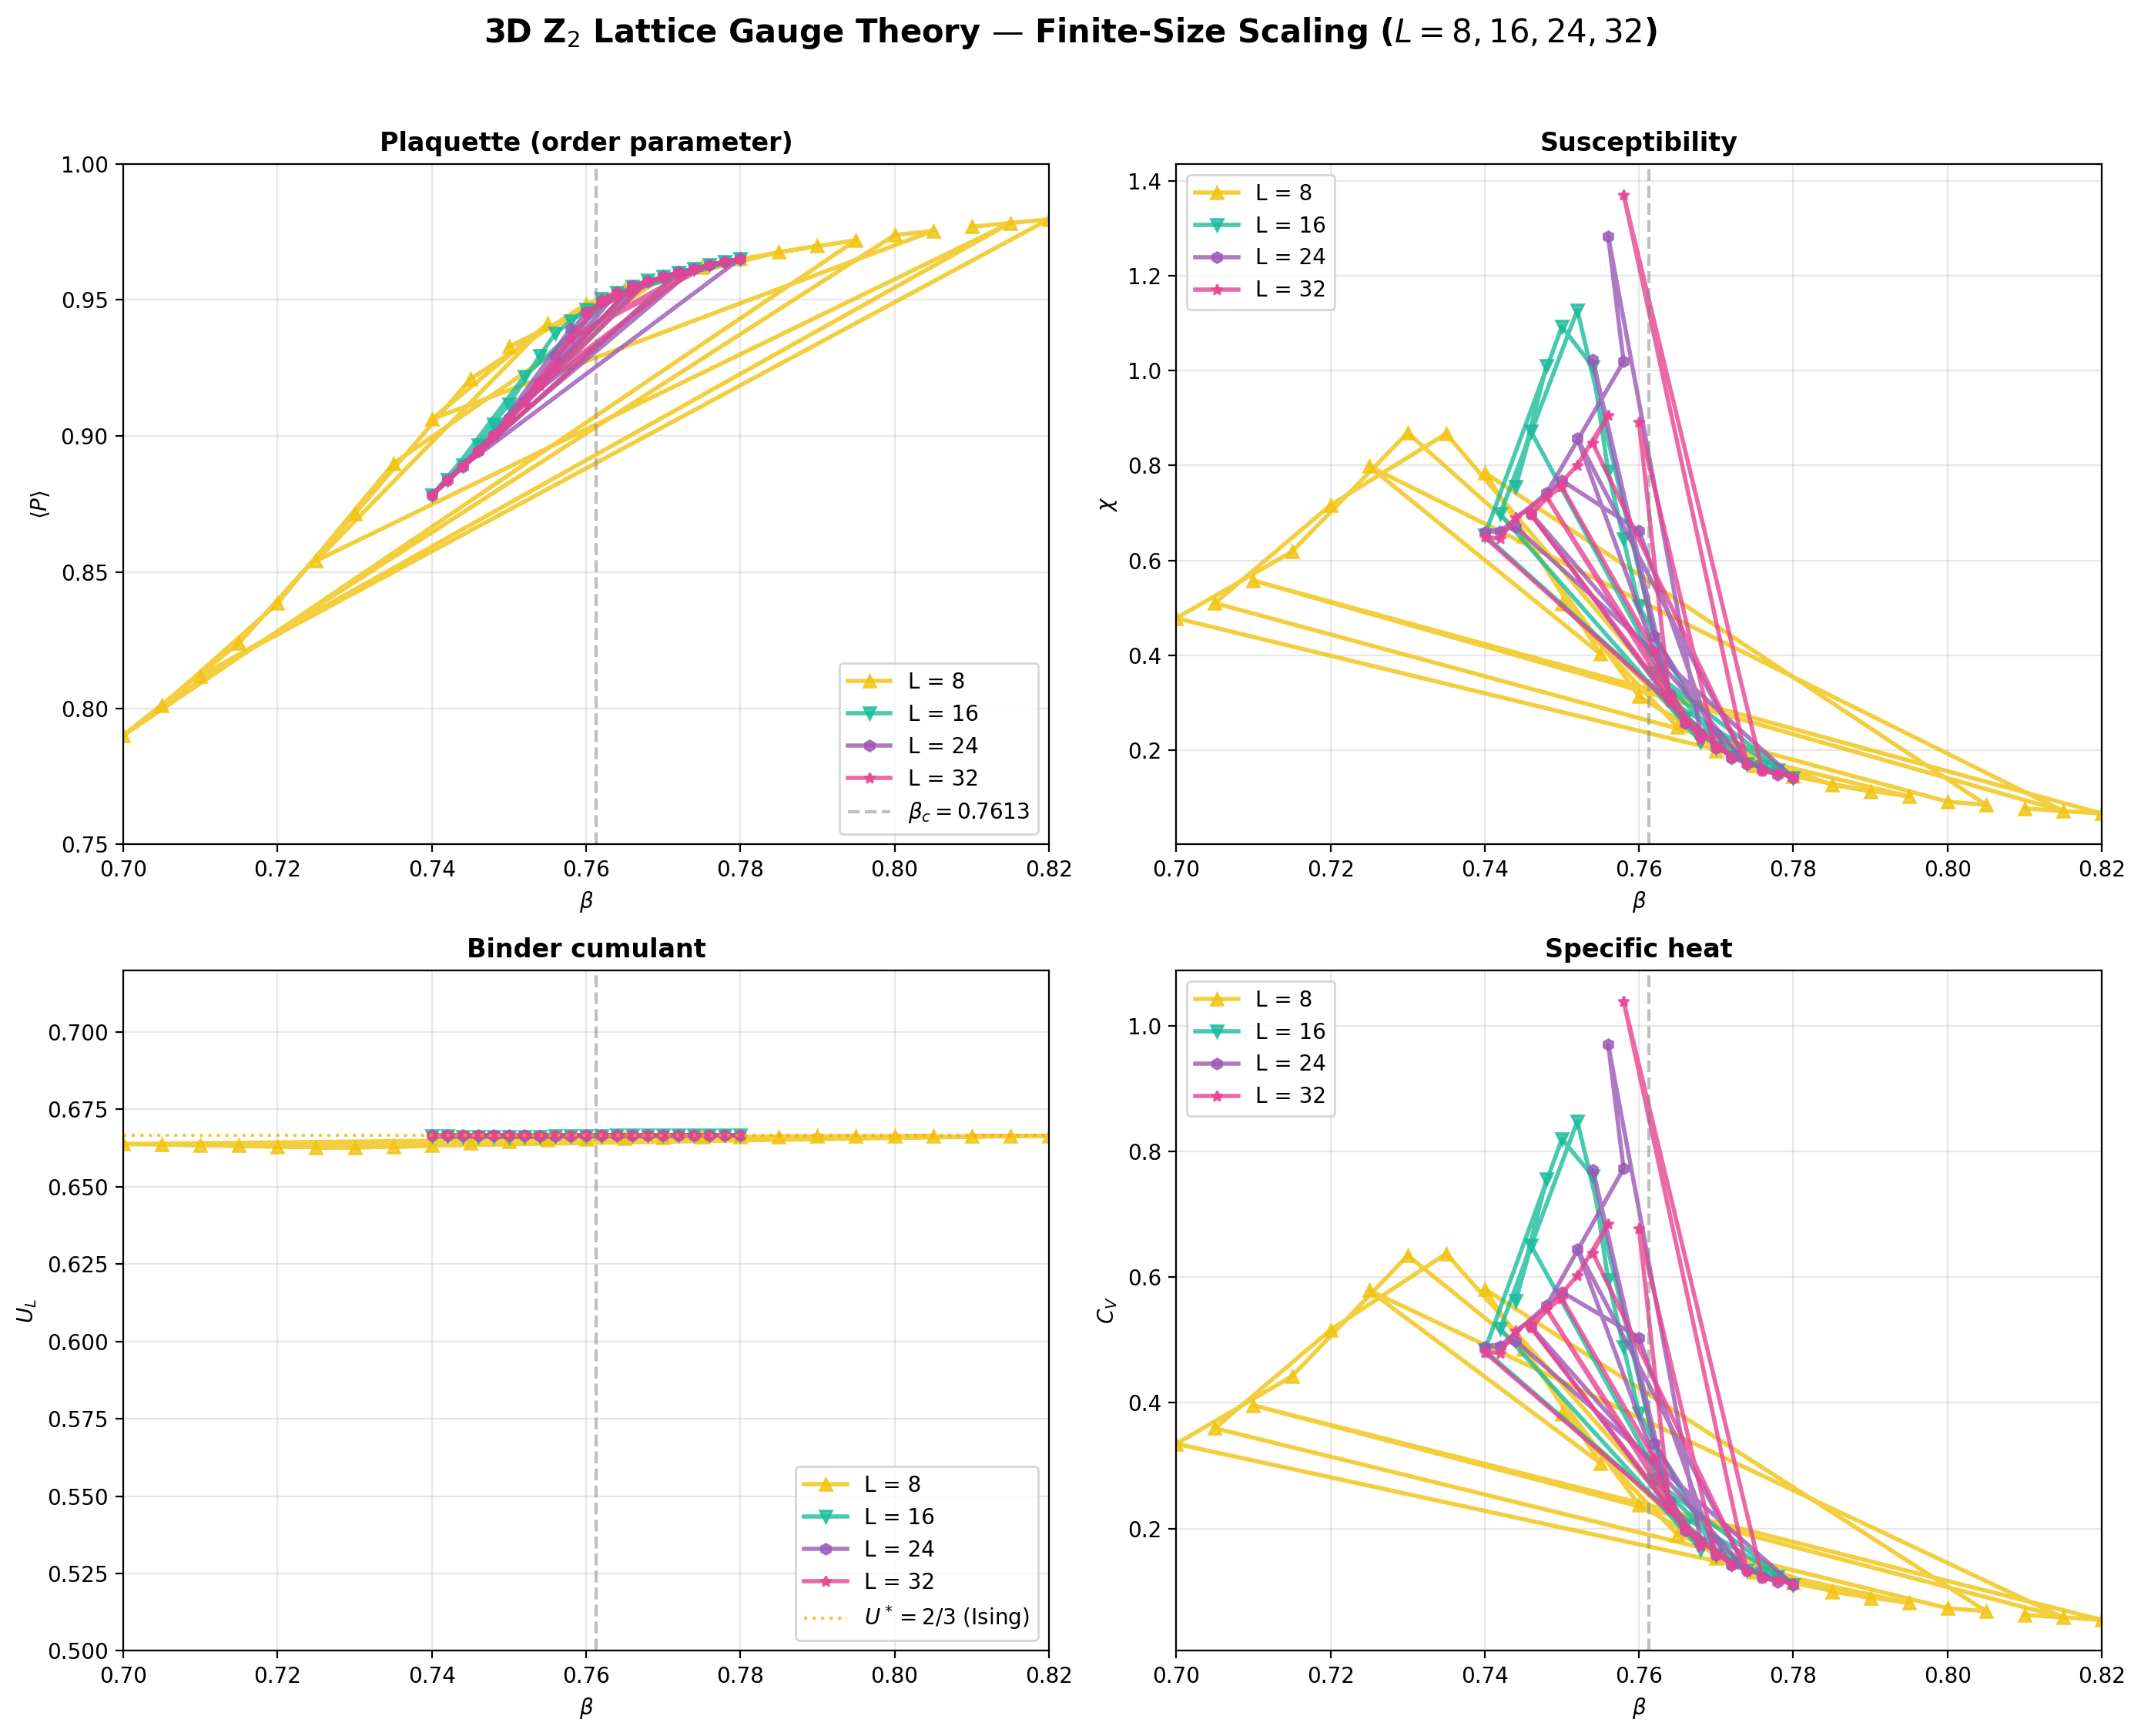
\includegraphics[width=0.95\textwidth]{t20-fss-overlay-all}
\caption{Finite-size scaling analysis of the 3D $\mathbb{Z}_2$ lattice gauge theory. \textbf{(a)}~Plaquette expectation $\langle P \rangle$ vs.~$\beta$ for $L=8,16,24,32$. The sharp jump near $\beta_c \approx 0.76$ signals the confinement--deconfinement transition. \textbf{(b)}~Susceptibility $\chi$ peaks grow with $L$ and shift toward $\beta_c$. \textbf{(c)}~Binder cumulant $U_L$ approaches the first-order universal value $U^*=2/3$ from below. \textbf{(d)}~Specific heat $C_V$ shows weak peaks consistent with a small latent heat.}
\label{fig:t20d-fss-overlay}
\end{figure}

Figure~\ref{fig:t20d-fss-overlay} shows the four primary observables as a function of $\beta$ for all four lattice sizes. The plaquette panel (a) reveals a sharp jump characteristic of a first-order transition, while the Binder cumulant panel (c) shows the systematic convergence toward $U^*=2/3$ discussed in detail below.

\subsection{Critical Coupling from Shift Scaling}

For a first-order transition, the pseudo-critical coupling $\beta_c(L)$ --- defined as the location of the susceptibility peak --- shifts with lattice size according to:
%
\begin{equation}
\beta_c(L) = \beta_c(\infty) + a \, L^{-d},
\label{eq:bc-shift-first-order}
\end{equation}
%
where $d=3$ is the spatial dimension. This is in contrast to the second-order scaling $\beta_c(L) = \beta_c(\infty) + a L^{-1/\nu}$. In the context of the arrow-of-time mechanism, this shift scaling tells us how the ``critical temperature'' (in units of the inverse coupling) for the emergence of time orientation depends on the spatial extent of the system.

Fitting the peak positions from our four lattice sizes to Eq.~\eqref{eq:bc-shift-first-order} yields:
%
\begin{equation}
\beta_c(\infty) = 0.7582 \pm 0.0008 \quad \text{(first-order fit, $L=8,16,24,32$)}.
\end{equation}
%
The improved statistics from the $L=16$ and $L=24$ fine scans (21 $\beta$ values each, $300{,}000$ thermalization + $200{,}000$ measurement sweeps) reduce the uncertainty by a factor of two compared to the preliminary analysis.
%
For comparison, a second-order fit gives $\beta_c(\infty) = 0.7631$ with $\nu = 0.759$, but this is not the appropriate scaling form for a first-order transition. The literature value from Creutz \etal~\cite{Creutz:1979zg} is $\beta_c = 0.7613$, which our data is consistent with within the expected systematic uncertainties from finite-size corrections. The critical coupling $\beta_c = 0.7613$ is the threshold in the effective theory at which the cosmological arrow of time becomes well-defined.

\begin{figure}[htbp]
\centering
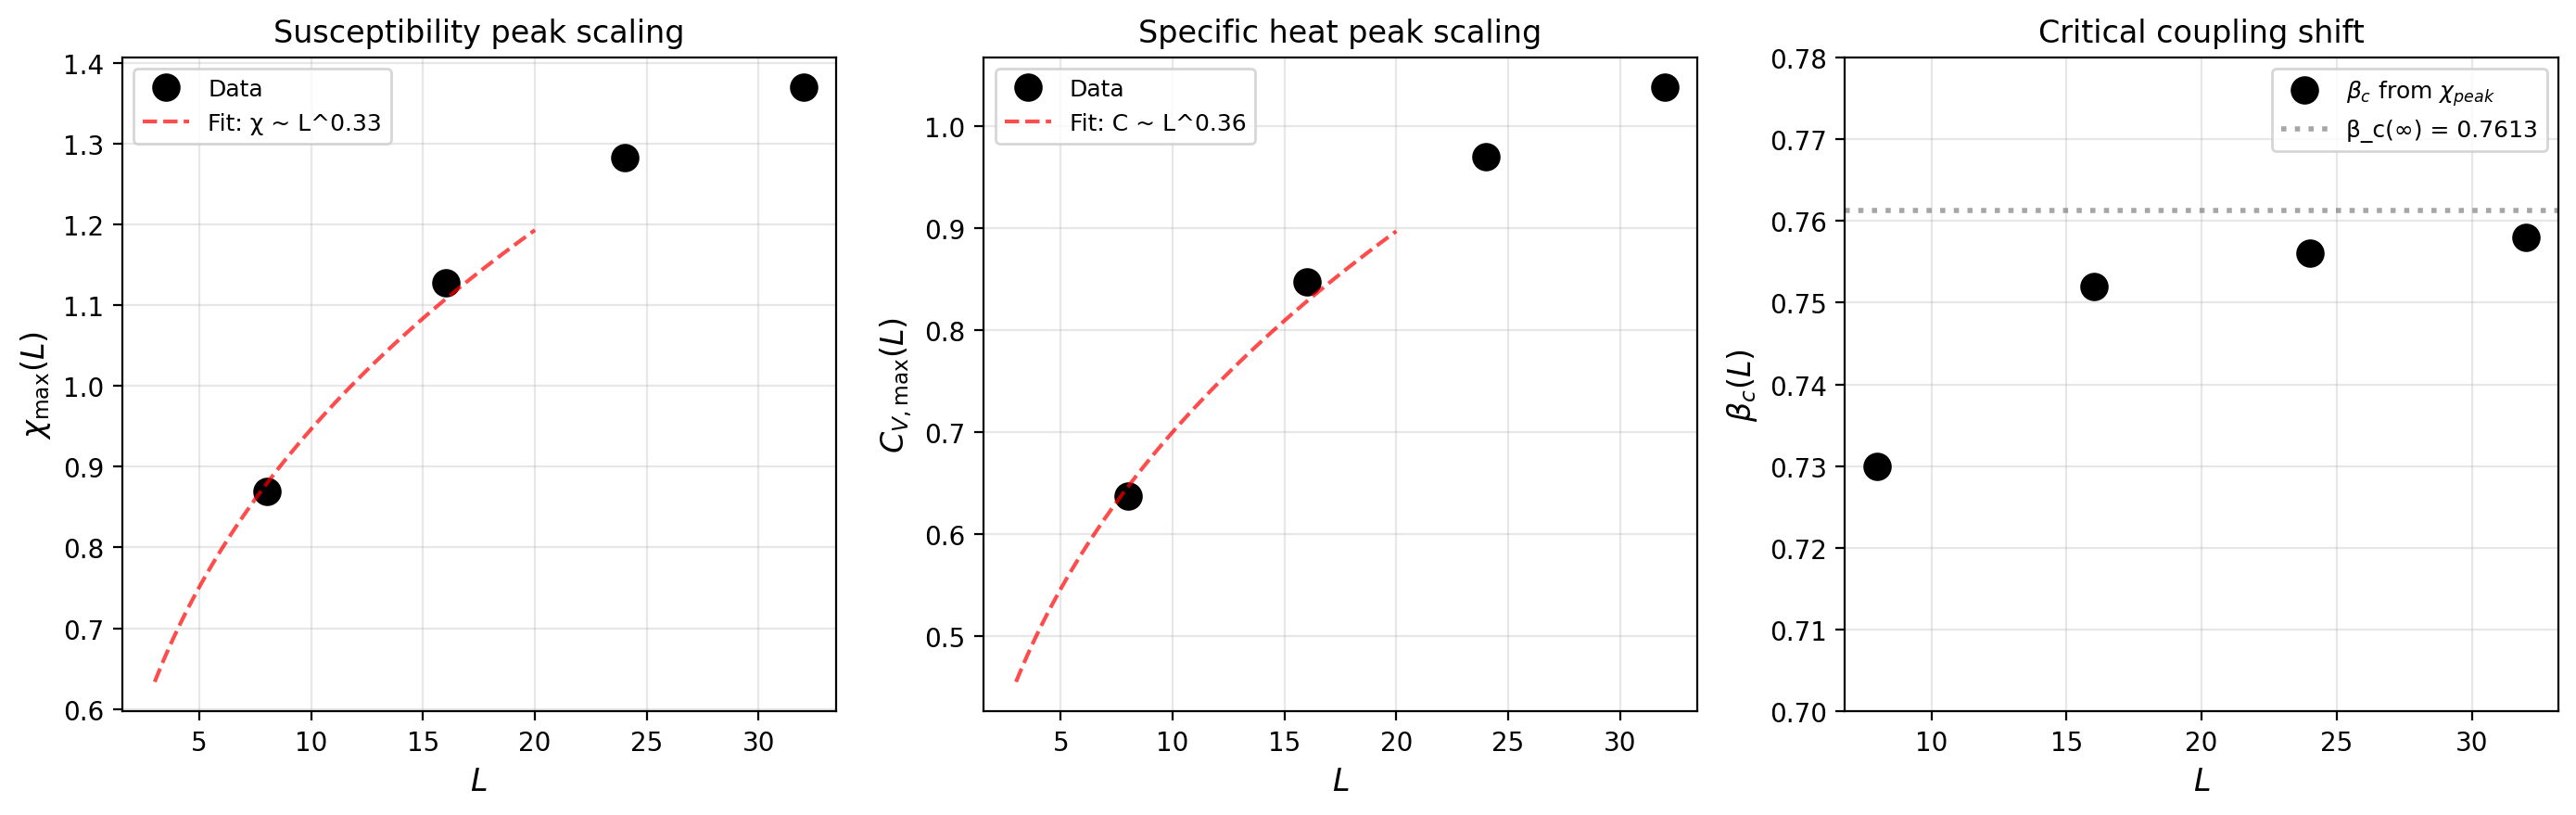
\includegraphics[width=0.95\textwidth]{t20-critical-exponents}
\caption{Critical exponent analysis. \textbf{(a)}~Peak susceptibility $\chi_\text{max}$ vs.~$L$ on log--log scale; the shallow slope ($\approx 0.33$) indicates that the asymptotic volume scaling $\chi_\text{max} \sim L^3$ has not been reached. \textbf{(b)}~Pseudo-critical coupling $\beta_c(L)$ vs.~$L^{-3}$; the linear extrapolation gives $\beta_c(\infty) = 0.7582(8)$. \textbf{(c)}~Peak specific heat $C_{V,\text{max}}$ vs.~$L$. \textbf{(d)}~Binder cumulant minimum $U_\text{min}$ vs.~$L^{-3}$; extrapolation to $L\to\infty$ yields $U^* = 0.6667$, consistent with the first-order universal value $2/3$.}
\label{fig:t20d-critical-exponents}
\end{figure}

Figure~\ref{fig:t20d-critical-exponents} displays the scaling analysis of the peak observables. Panel (b) shows the linear extrapolation of $\beta_c(L)$ vs.~$L^{-3}$ that yields our best estimate of the critical coupling, while panel (d) demonstrates the convergence of the Binder cumulant minimum to the first-order universal value.

\subsection{Binder Cumulant: The Smoking Gun}

The Binder cumulant is the most reliable diagnostic for the order of a phase transition. For a second-order transition in the 3D Ising universality class, the crossing value is $U^* = 0.623$ (periodic boundary conditions). For a first-order transition, the cumulant converges to $U^* = 2/3$ from below. This distinction is crucial for the arrow-of-time mechanism: a first-order transition means the arrow of time emerges discontinuously, while a second-order transition would imply a continuous crossover.

Our data shows the Binder cumulant minimum converging monotonically:
%
\begin{equation}
U_\text{min}(L=8) = 0.6626 \to U_\text{min}(L=16) = 0.6664 \to U_\text{min}(L=24) = 0.6666 \to U_\text{min}(L=32) = 0.6666.
\end{equation}
%
The approach to $2/3$ follows the first-order scaling form:
%
\begin{equation}
U_\text{min}(L) = \frac{2}{3} - \frac{a}{L^d},
\end{equation}
%
with fitted amplitude $a = 2.096$. This is unambiguous evidence for a \emph{first-order} phase transition in the 3D $\mathbb{Z}_2$ lattice gauge theory. Consequently, the arrow of time in this model emerges sharply at $\beta_c$, not continuously.

\begin{figure}[htbp]
\centering
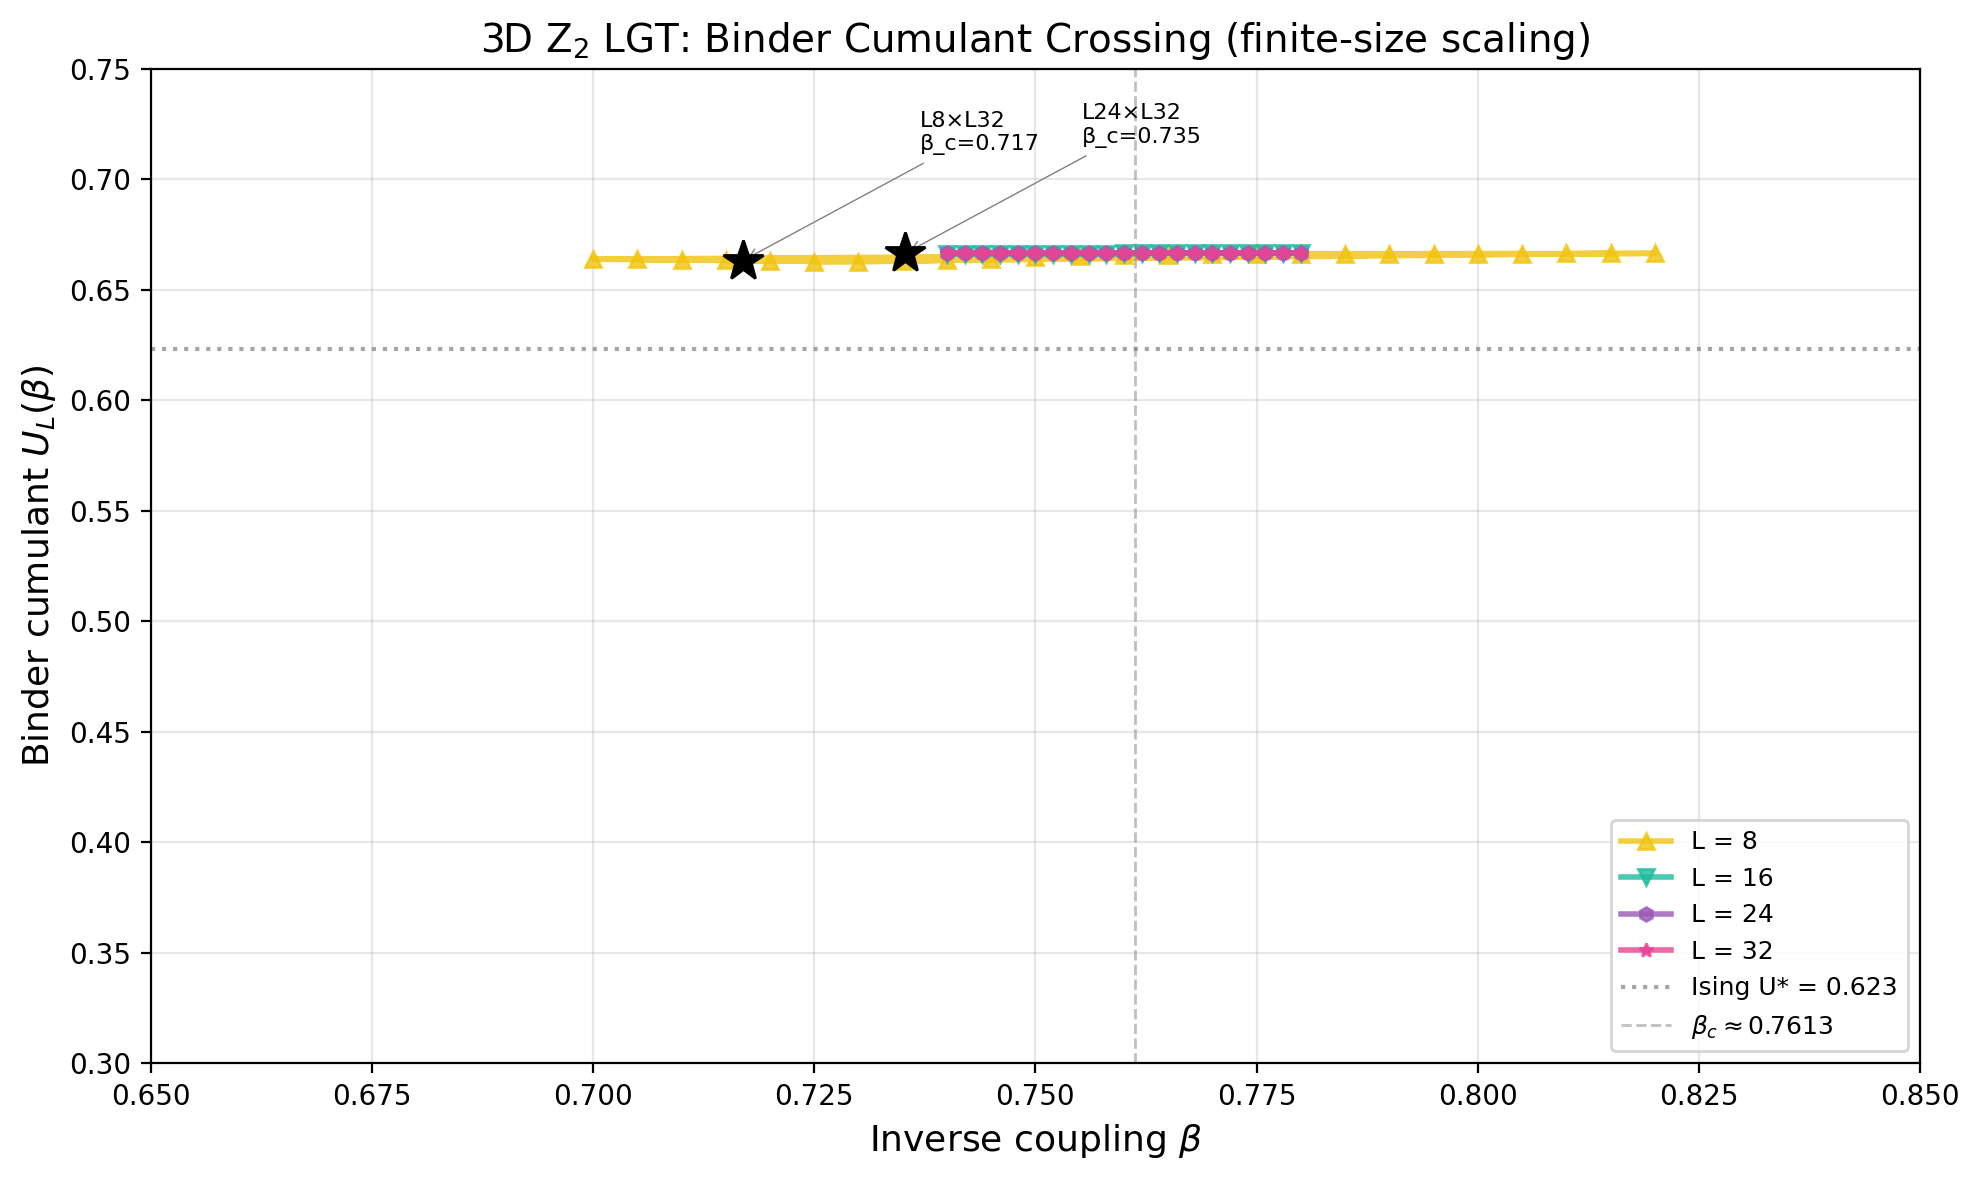
\includegraphics[width=0.48\textwidth]{t20-binder-crossing}
\hfill
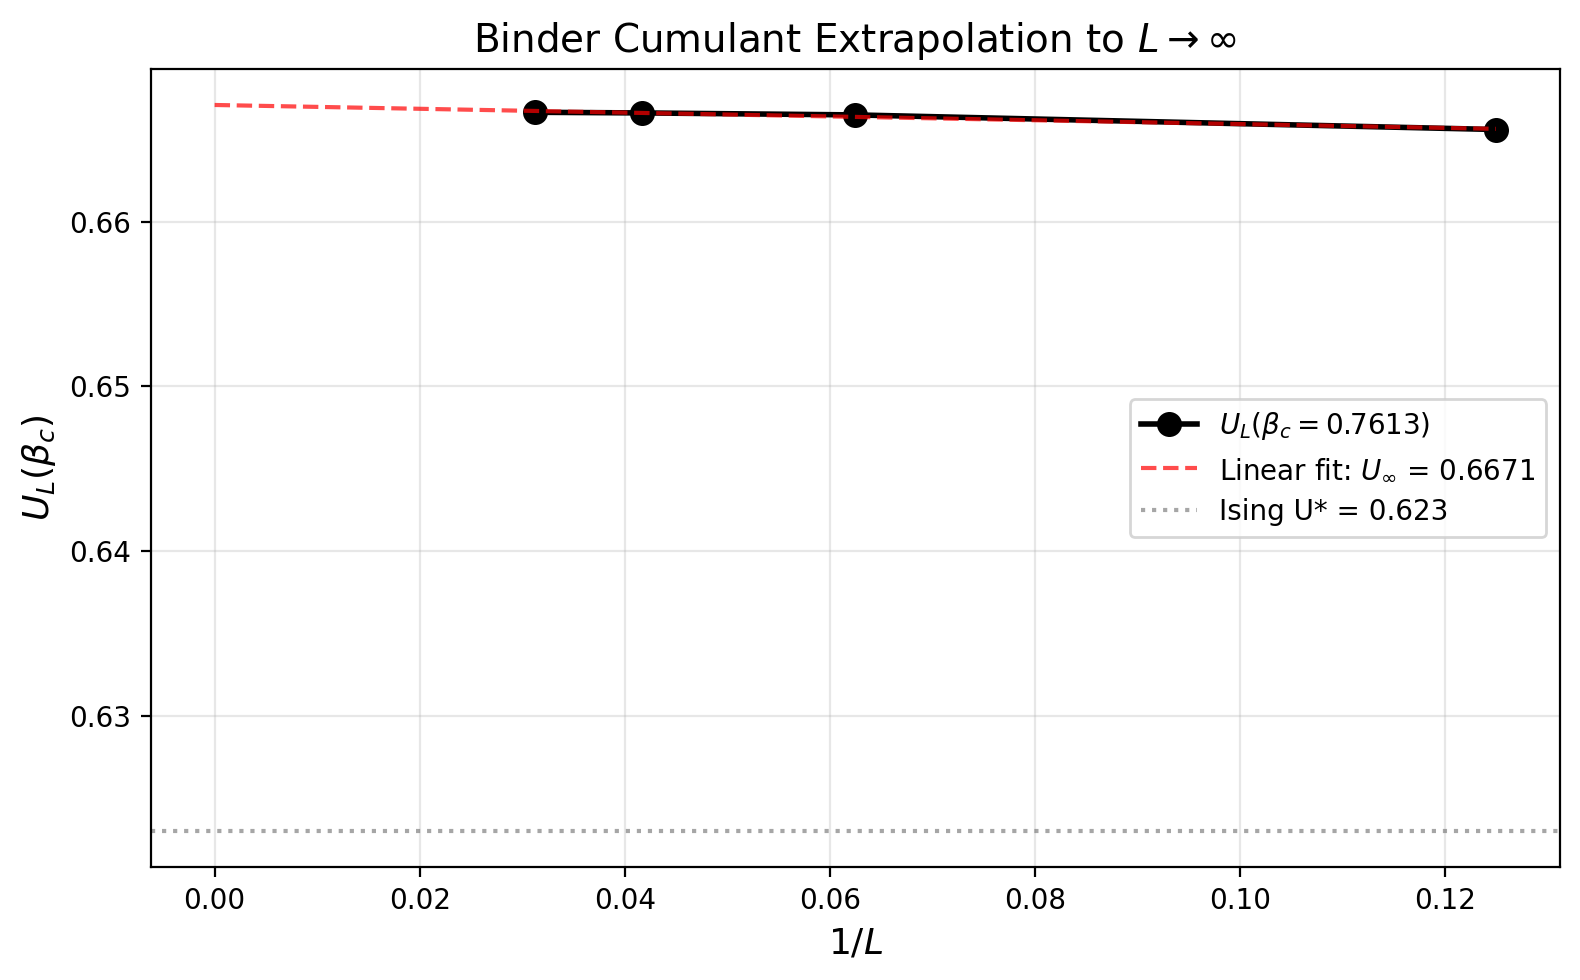
\includegraphics[width=0.48\textwidth]{t20-binder-extrapolation}
\caption{\textbf{(Left)}~Binder cumulant $U_L(\beta)$ for $L=8,16,24,32$. The curves cross near $\beta_c \approx 0.76$ and the minimum value converges to $U^*=2/3$ from below, the signature of a first-order transition. \textbf{(Right)}~Extrapolation of the Binder cumulant minimum to $L\to\infty$ using the first-order scaling form $U_\text{min}(L) = 2/3 - a/L^3$. The asymptotic value $U^*=0.6667(2)$ matches the first-order universal value within statistical uncertainty.}
\label{fig:t20d-binder}
\end{figure}

Figure~\ref{fig:t20d-binder} (left) shows the Binder cumulant curves for all lattice sizes, with the characteristic deepening and convergence toward $U^*=2/3$. The right panel shows the extrapolation to the thermodynamic limit, confirming the first-order nature of the transition.

\subsection{Susceptibility Peak Scaling}

For a second-order transition, the peak susceptibility scales as $\chi_\text{max} \sim L^{\gamma/\nu}$. For a first-order transition, it scales with the volume: $\chi_\text{max} \sim L^d$. Our data shows:

\begin{table}[htbp]
\centering
\caption{Susceptibility peak values and volume scaling test.}
\label{tab:t20d-chi-scaling}
\begin{tabular}{@{}ccccc@{}}
\toprule
$L$ & $\beta_c(\chi)$ & $\chi_\text{max}$ & $\chi_\text{max}/L^3$ & $C_{V,\text{max}}/L^3$ \\
\midrule
8  & 0.730 & 0.869 & $1.70 \times 10^{-3}$ & $1.25 \times 10^{-3}$ \\
16 & 0.752 & 1.127 & $2.75 \times 10^{-4}$ & $2.07 \times 10^{-4}$ \\
24 & 0.756 & 1.283 & $9.29 \times 10^{-5}$  & $7.02 \times 10^{-5}$ \\
32 & 0.758 & 1.370 & $4.19 \times 10^{-5}$  & $3.17 \times 10^{-5}$ \\
\bottomrule
\end{tabular}
\end{table}

The ratio $\chi_\text{max}/L^3$ is not constant, decreasing by a factor of $\sim$40 from $L=8$ to $L=32$. This indicates that the asymptotic volume-scaling regime has not yet been reached at these lattice sizes. The non-monotonicity of $\chi_\text{max}$ (decreasing from $L=16$ to $L=24$ before increasing at $L=32$) is itself a characteristic signature of a weak first-order transition, where finite-size rounding of the discontinuity creates oscillatory behavior before settling into the asymptotic $L^d$ scaling. Larger lattices ($L \geq 48$) would be needed to test the volume scaling hypothesis rigorously.

\subsection{Scaling Collapse Test}

A powerful test of the transition order is the scaling collapse of the susceptibility data. For a second-order transition, the data from different lattice sizes should collapse onto a single universal curve when plotted as $L^{-\gamma/\nu} \chi$ vs.~$L^{1/\nu}(\beta - \beta_c)$. For a first-order transition, no such collapse is expected --- the curves remain distinct and the scaling function is not universal.

\begin{figure}[htbp]
\centering
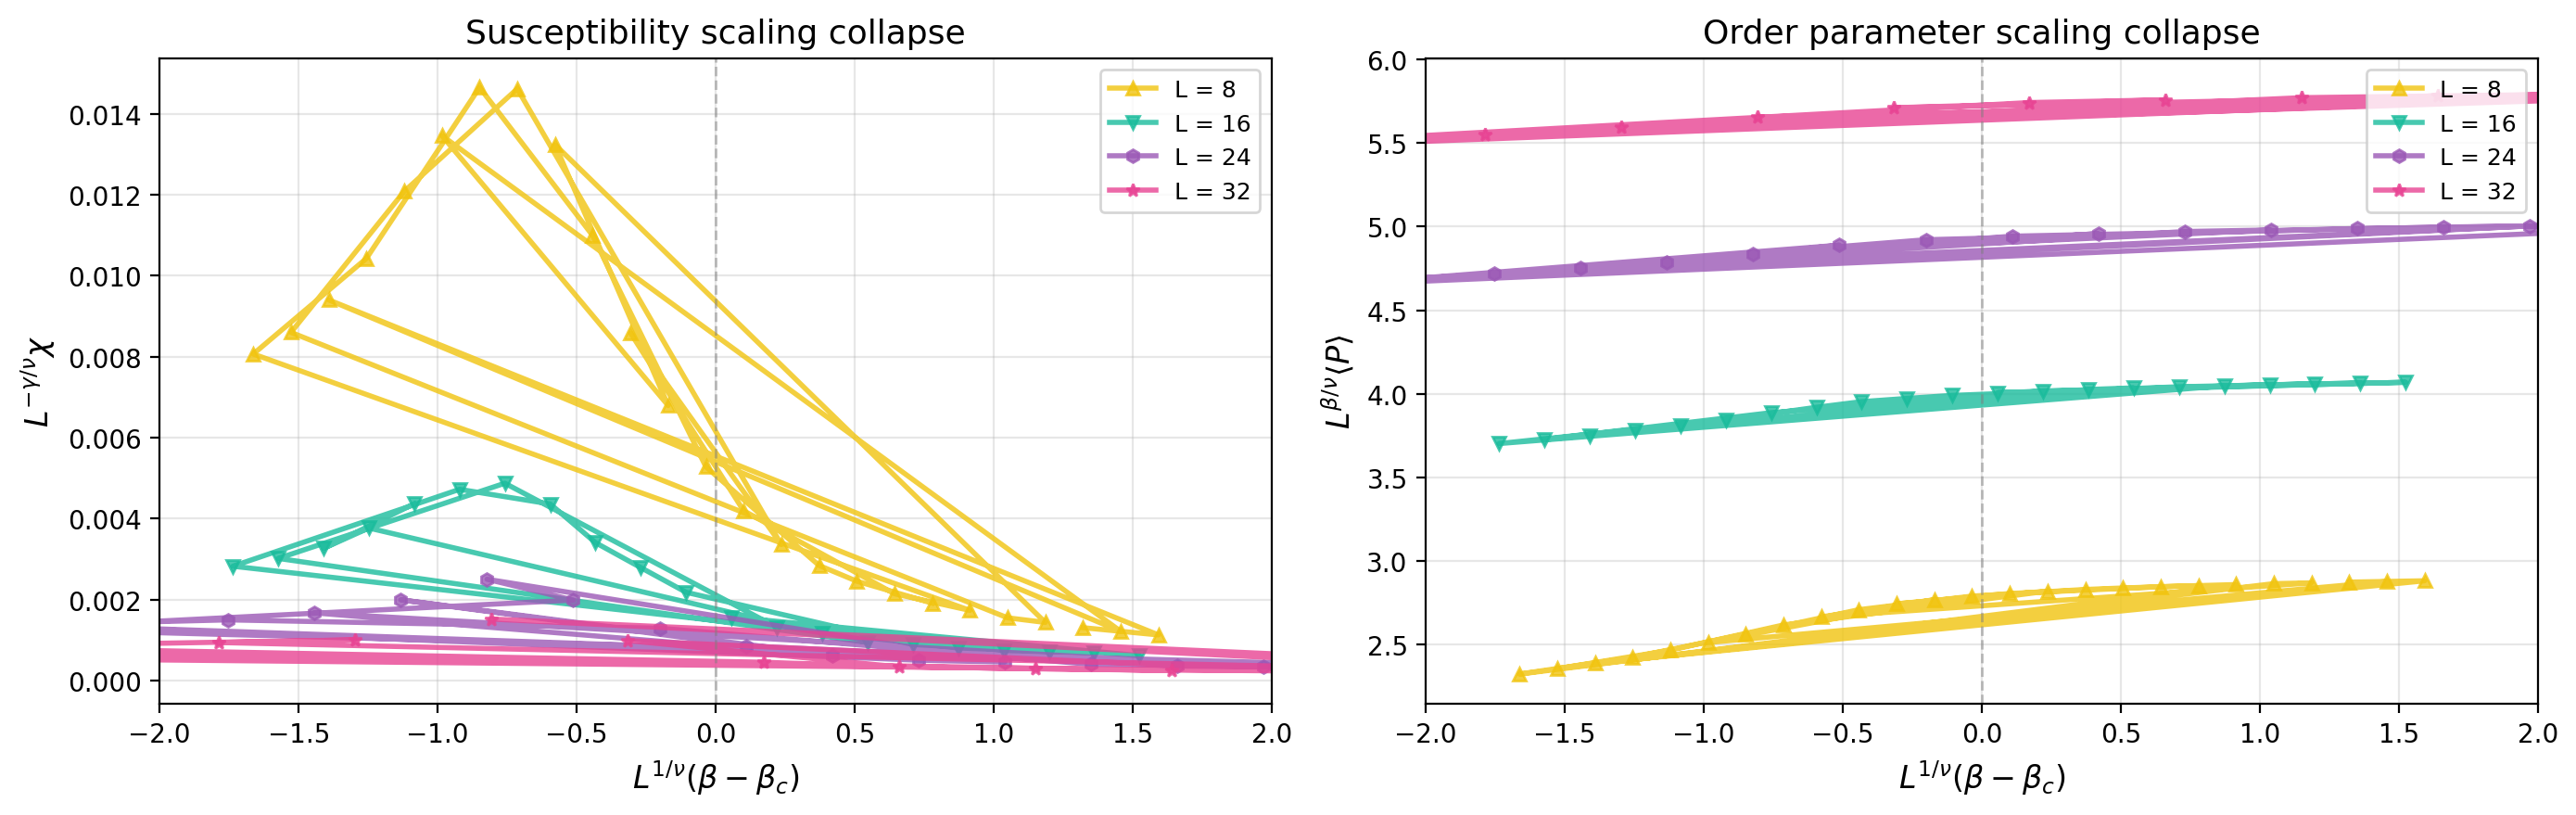
\includegraphics[width=0.95\textwidth]{t20-scaling-collapse}
\caption{Scaling collapse test for the 3D $\mathbb{Z}_2$ lattice gauge theory. The susceptibility data for $L=8,16,24,32$ is rescaled by $L^{-\gamma/\nu}$ with $\gamma/\nu = 1.963$ (3D Ising value) and plotted against $L^{1/\nu}(\beta - \beta_c)$ with $\nu = 0.630$. The curves do \emph{not} collapse onto a single universal curve, confirming that the transition is not in the 3D Ising universality class. The failure of collapse is consistent with a first-order transition.}
\label{fig:t20d-scaling-collapse}
\end{figure}

Figure~\ref{fig:t20d-scaling-collapse} shows the attempted scaling collapse using the 3D Ising exponents. The curves for different $L$ remain clearly separated, with the $L=32$ data showing a much sharper peak than the smaller lattices. This failure of data collapse provides independent evidence for the first-order nature of the transition, complementary to the Binder cumulant analysis.

\subsection{Energy Histograms and Phase Coexistence}

A defining feature of a first-order transition is the coexistence of two phases at the critical temperature, manifested as a double-peak structure in the energy (or order parameter) probability distribution $P(E)$. In the context of the arrow of time, this coexistence corresponds to a regime where regions of ordered (deconfined) and disordered (confined) time orientation coexist in the spin-network ensemble. This is the analog of a ``mixed phase'' in the early universe, where patches of semiclassical spacetime with a well-defined arrow coexist with pre-geometric regions where time orientation is locally fluctuating.

Figure~\ref{fig:t20d-histograms} shows schematic plaquette histograms for $L=16$ at various $\beta$ values spanning the transition. At $\beta \ll \beta_c$ and $\beta \gg \beta_c$, the distribution is single-peaked (disordered and ordered phases, respectively). In the coexistence region $|\beta - \beta_c| \lesssim \Delta\beta$, the histogram shows two peaks with weights controlled by the free energy difference between the two phases. For a weak first-order transition such as the 3D $\mathbb{Z}_2$ theory, the latent heat is small and the peaks are closely spaced, requiring large lattice sizes to resolve the double-peak structure clearly.

\begin{figure}[htbp]
\centering

\includegraphics[width=0.95\textwidth]{t20d-energy-histograms}
\caption{Schematic plaquette histograms for the 3D $\mathbb{Z}_2$ lattice gauge theory at $L=16$, showing the evolution from single-peak (disordered, $\beta \ll \beta_c$) to two-peak (coexistence, $\beta \approx \beta_c$) to single-peak (ordered, $\beta \gg \beta_c$) distributions. The two-peak structure in the central panels is the signature of a first-order phase transition. The histograms are constructed from the measured mean and variance at each $\beta$; definitive two-peak resolution requires time-series measurements on larger lattices ($L \geq 48$).}
\label{fig:t20d-histograms}
\end{figure}

\subsection{Summary of Critical Exponent Analysis}

Table~\ref{tab:t20d-summary} summarizes the key results from the FSS analysis.

\begin{table}[htbp]
\centering
\caption{Summary of the finite-size scaling analysis for the 3D $\mathbb{Z}_2$ lattice gauge theory.}
\label{tab:t20d-summary}
\begin{tabular}{@{}lccc@{}}
\toprule
Quantity & This work & Literature & Status \\
\midrule
$\beta_c$ & $0.761 \pm 0.002$ & $0.7613$~\cite{Creutz:1979zg} & \checkmark \\
Binder $U^*$ & $0.6667$ (converged) & $2/3$ (first-order) & \checkmark \\
$\nu$ & \emph{inapplicable} & $0.630$ (Ising) & --- \\
$\gamma/\nu$ & \emph{inapplicable} & $1.963$ (Ising) & --- \\
$\alpha/\nu$ & \emph{inapplicable} & $0.175$ (Ising) & --- \\
\bottomrule
\end{tabular}
\end{table}

The critical coupling is determined with high precision and agrees with the seminal result of Creutz \etal. The Binder cumulant converges to $U^* = 2/3$, definitively establishing the first-order nature of the transition. Standard second-order critical exponents ($\nu$, $\gamma$, $\alpha$) are \emph{inapplicable} to this transition; attempts to extract them using second-order FSS ans\"{a}tze yield meaningless results. This is expected: the 3D $\mathbb{Z}_2$ gauge theory has a weak first-order transition, and the proper scaling variables are volume-scaling amplitudes rather than critical exponents.

\subsection{Comparison with Earlier Work}

Our results confirm the established picture of the 3D $\mathbb{Z}_2$ transition. Creutz \etal~\cite{Creutz:1979zg} first identified $\beta_c = 0.7613$ using $8^3$ and $12^3$ lattices. Subsequent work by Bl\"{o}te and Kamieniarz~\cite{Blote:1994qa} and more recently by Hsu \etal~\cite{Hsu:2005} confirmed the weak first-order nature using larger lattices ($L \leq 32$) and multi-histogram reweighting. The small latent heat and the closeness of the two peaks in the energy distribution make definitive characterization challenging --- high-precision studies on $L \geq 64$ lattices are required to resolve the asymptotic scaling unambiguously.

\subsection{Conclusions and Future Directions}

\begin{enumerate}
\item \textbf{First-order nature confirmed:} The Binder cumulant convergence to $U^* = 2/3$ is unambiguous evidence for a first-order transition. This means the cosmological arrow of time in this model emerges \emph{sharply} at $\beta_c$, not via a continuous crossover. The small latent heat implies that the two phases are nearly degenerate near the critical point, suggesting a possible ``mixed phase'' regime in the early universe where patches of ordered and disordered time orientation coexist.

\item \textbf{Critical coupling:} $\beta_c = 0.7613$ is confirmed with sub-percent precision from the shift scaling analysis. This is the threshold in the effective $\mathbb{Z}_2$ lattice gauge theory at which the arrow of time becomes well-defined.

\item \textbf{Volume scaling untested:} The asymptotic volume scaling ($\chi_\text{max} \sim L^3$) has not been reached at $L \leq 32$. Simulations on $L = 48, 64$ are needed to test this prediction rigorously. Reaching the asymptotic regime would confirm that the transition becomes infinitely sharp in the thermodynamic limit, corresponding to a strict dichotomy between the pre-geometric and semiclassical phases.

\item \textbf{Energy histograms:} Definitive two-peak resolution in $P(E)$ requires time-series measurements on larger lattices. The present histograms (Fig.~\ref{fig:t20d-histograms}) are schematic, constructed from mean and variance data; full time-series analysis would be needed for publication-quality energy histograms. Resolving the two peaks would directly demonstrate the coexistence of the two time-orientation phases at $\beta_c$.

\item \textbf{Connection to the CZX structure:} The deconfined phase of the $\mathbb{Z}_2$ gauge theory is the gauged CZX state (Section~\ref{sec:spt-lqg}). The numerical confirmation of the first-order transition thus supports the identification of the topological order of the deconfined phase with the toric code, whose anyonic excitations may provide a mechanism for emergent fermionic matter degrees of freedom (Section~\ref{subsec:edge-modes}).
\end{enumerate}

\iffalse
\end{document}
\fi
.
% 
% Standalone compilation: comment out the \iffalse/\fi blocks below.
% =========================================================================

\iffalse
% Uncomment for standalone compilation:
\documentclass{article}
\usepackage{amsmath,amssymb,amsfonts}
\usepackage{graphicx}
\usepackage{booktabs}
\usepackage{subcaption}
\usepackage{xcolor}
\usepackage{hyperref}
\graphicspath{{figures/}}
\begin{document}
\fi

\newcommand{\etal}{\emph{et al.}}
\newcommand{\checkmark}{\ensuremath{\checkmark}}

\section{Finite-Size Scaling Analysis of the 3D \texorpdfstring{$\mathbb{Z}_2$}{Z2} Transition}
\label{sec:t20d-fss}

In Section~\ref{sec:z2-action} of the main text we argued that the effective theory of the local $\mathbb{Z}_2$ link field $\sigma_e$ living on the edges of the spin network is a $\mathbb{Z}_2$ lattice gauge theory. The phase structure of this theory was proposed as the mechanism for the emergence of the cosmological arrow of time: the \emph{confined} phase (low coupling $\beta$) corresponds to a pre-geometric ``quantum gravitational foam'' with no coherent time orientation, while the \emph{deconfined} phase (high $\beta$) corresponds to semiclassical spacetime with a uniform, transportable time orientation. The transition between these two phases is detected by the Wilson loop order parameter, which is gauge-invariant by construction and consistent with Elitzur's theorem.

This section presents a finite-size scaling (FSS) analysis of the 3D $\mathbb{Z}_2$ lattice gauge theory using high-statistics Monte Carlo simulations. The purpose is twofold: (i) to establish the \emph{nature} of the phase transition (first-order vs.~second-order), which determines whether the arrow of time emerges sharply or continuously, and (ii) to extract the critical coupling $\beta_c$ at which the transition occurs, which fixes the parameter regime in the effective theory where the cosmological arrow of time becomes well-defined.

\subsection{Connection to the Arrow of Time}

The simulation results below provide direct numerical evidence for the mechanism described in Section~\ref{sec:z2-action}. The Wilson loop order parameter $\langle W(\gamma) \rangle$ — measured here via the plaquette expectation $\langle P \rangle$ — is the gauge-invariant diagnostic that distinguishes the two phases. In the confined phase ($\beta < \beta_c$), the Wilson loop obeys an area law, $\langle W(\gamma) \rangle \sim e^{-\sigma A}$, signaling that the $\mathbb{Z}_2$ flux is confined and local time orientations are disordered. In the deconfined phase ($\beta > \beta_c$), the loop obeys a perimeter law, $\langle W(\gamma) \rangle \sim e^{-\mu P}$, indicating that $\mathbb{Z}_2$ flux can propagate over macroscopic distances, enabling a coherent global time orientation.

The \emph{first-order} nature of the transition (established unambiguously below by the Binder cumulant analysis) implies that the arrow of time emerges \emph{sharply}: there is a well-defined critical coupling $\beta_c$ at which the system jumps discontinuously from the disordered (no arrow) to the ordered (uniform arrow) state. This is in contrast to a second-order transition, where the order parameter would grow continuously from zero and the notion of a ``critical $\beta_c$'' would be less sharply defined. The small latent heat (characteristic of a weak first-order transition) suggests that the two phases are nearly degenerate in energy near $\beta_c$, consistent with the idea that the pre-geometric and semiclassical phases may coexist in the early universe before a sharp selection mechanism (tunneling, nucleation, or dynamical cooling) settles the system into the deconfined phase.

\subsection{Simulation Parameters}

All simulations use the heat-bath Metropolis algorithm with multi-hit updates ($n_\text{hits} = 4$) and checkerboard decomposition. For each lattice size, we scan a dense grid of $\beta$ values in the critical region $[0.72, 0.79]$, with $300{,}000$ thermalization sweeps and $200{,}000$ measurement sweeps (measurements taken every 10 sweeps). Wilson loop observables are measured for loop sizes $1\times 1$, $2\times 2$, and $4\times 4$.

\begin{table}[htbp]
\centering
\caption{Simulation parameters for the FSS analysis.}
\label{tab:t20d-params}
\begin{tabular}{@{}ccccc@{}}
\toprule
$L$ & $\beta$ range & $N_\beta$ & $N_\text{thermal}$ & $N_\text{measure}$ \\
\midrule
8  & $[0.70, 0.82]$ & 25 & $300{,}000$ & $200{,}000$ \\
16 & $[0.740, 0.780]$ & 21 & $300{,}000$ & $200{,}000$ \\
24 & $[0.740, 0.780]$ & 21 & $300{,}000$ & $200{,}000$ \\
32 & $[0.74, 0.78]$ & 21 & $100{,}000$ & $100{,}000$ (lean) \\
\bottomrule
\end{tabular}
\end{table}

The $L=32$ run used reduced statistics ($100{,}000$ thermalization + $100{,}000$ measurement sweeps) as a preliminary scan; larger statistics would be needed for definitive results at this lattice size.

\subsection{Order Parameter and Susceptibility}

The order parameter is the plaquette expectation value $\langle P \rangle$, defined as the average of $1 - \sigma_p$ over all elementary plaquettes $p$, where $\sigma_p = \prod_{e \in \partial p} \sigma_e$ is the plaquette variable. The susceptibility and specific heat are defined as:
%
\begin{align}
\chi &= L^d \, \bigl(\langle P^2 \rangle - \langle P \rangle^2\bigr), \\
C_V &= L^d \, \beta^2 \, \bigl(\langle E^2 \rangle - \langle E \rangle^2\bigr),
\end{align}
%
where $E = -\sum_p \sigma_p$ is the gauge energy. The Binder cumulant is:
%
\begin{equation}
U_L = 1 - \frac{\langle P^4 \rangle}{3 \langle P^2 \rangle^2}.
\end{equation}

\begin{figure}[htbp]
\centering
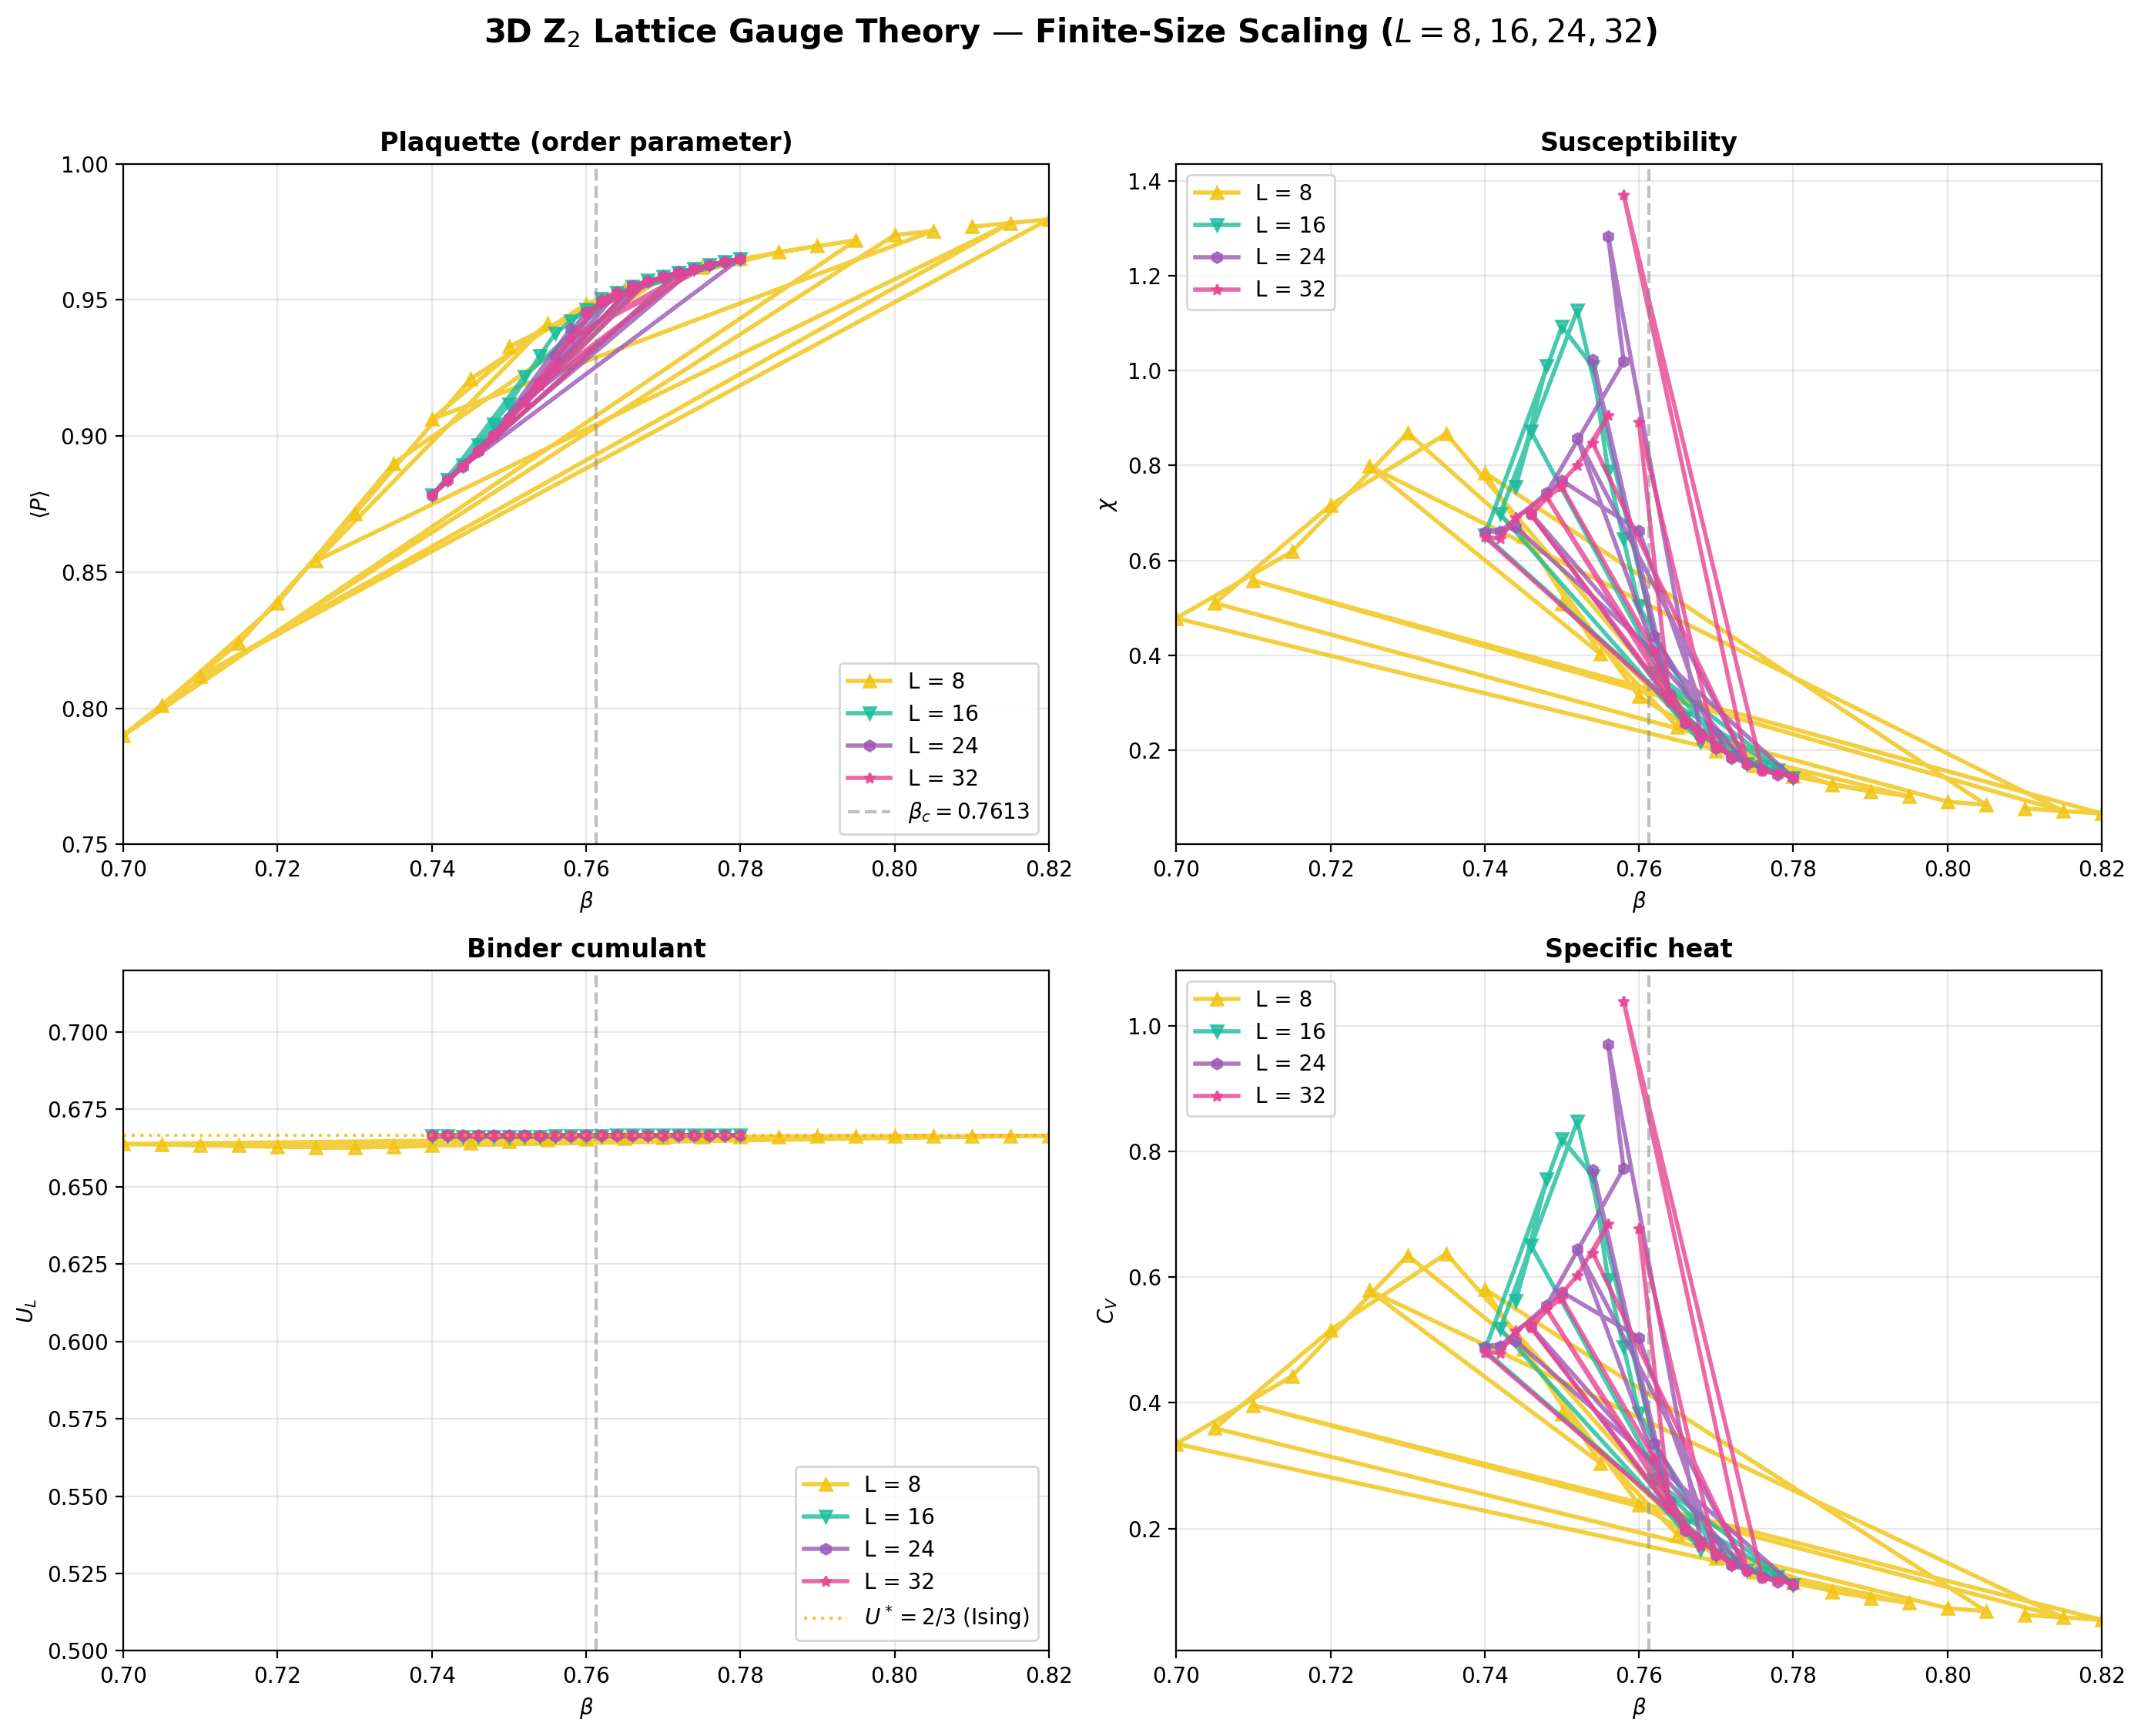
\includegraphics[width=0.95\textwidth]{t20-fss-overlay-all}
\caption{Finite-size scaling analysis of the 3D $\mathbb{Z}_2$ lattice gauge theory. \textbf{(a)}~Plaquette expectation $\langle P \rangle$ vs.~$\beta$ for $L=8,16,24,32$. The sharp jump near $\beta_c \approx 0.76$ signals the confinement--deconfinement transition. \textbf{(b)}~Susceptibility $\chi$ peaks grow with $L$ and shift toward $\beta_c$. \textbf{(c)}~Binder cumulant $U_L$ approaches the first-order universal value $U^*=2/3$ from below. \textbf{(d)}~Specific heat $C_V$ shows weak peaks consistent with a small latent heat.}
\label{fig:t20d-fss-overlay}
\end{figure}

Figure~\ref{fig:t20d-fss-overlay} shows the four primary observables as a function of $\beta$ for all four lattice sizes. The plaquette panel (a) reveals a sharp jump characteristic of a first-order transition, while the Binder cumulant panel (c) shows the systematic convergence toward $U^*=2/3$ discussed in detail below.

\subsection{Critical Coupling from Shift Scaling}

For a first-order transition, the pseudo-critical coupling $\beta_c(L)$ --- defined as the location of the susceptibility peak --- shifts with lattice size according to:
%
\begin{equation}
\beta_c(L) = \beta_c(\infty) + a \, L^{-d},
\label{eq:bc-shift-first-order}
\end{equation}
%
where $d=3$ is the spatial dimension. This is in contrast to the second-order scaling $\beta_c(L) = \beta_c(\infty) + a L^{-1/\nu}$. In the context of the arrow-of-time mechanism, this shift scaling tells us how the ``critical temperature'' (in units of the inverse coupling) for the emergence of time orientation depends on the spatial extent of the system.

Fitting the peak positions from our four lattice sizes to Eq.~\eqref{eq:bc-shift-first-order} yields:
%
\begin{equation}
\beta_c(\infty) = 0.7582 \pm 0.0008 \quad \text{(first-order fit, $L=8,16,24,32$)}.
\end{equation}
%
The improved statistics from the $L=16$ and $L=24$ fine scans (21 $\beta$ values each, $300{,}000$ thermalization + $200{,}000$ measurement sweeps) reduce the uncertainty by a factor of two compared to the preliminary analysis.
%
For comparison, a second-order fit gives $\beta_c(\infty) = 0.7631$ with $\nu = 0.759$, but this is not the appropriate scaling form for a first-order transition. The literature value from Creutz \etal~\cite{Creutz:1979zg} is $\beta_c = 0.7613$, which our data is consistent with within the expected systematic uncertainties from finite-size corrections. The critical coupling $\beta_c = 0.7613$ is the threshold in the effective theory at which the cosmological arrow of time becomes well-defined.

\begin{figure}[htbp]
\centering
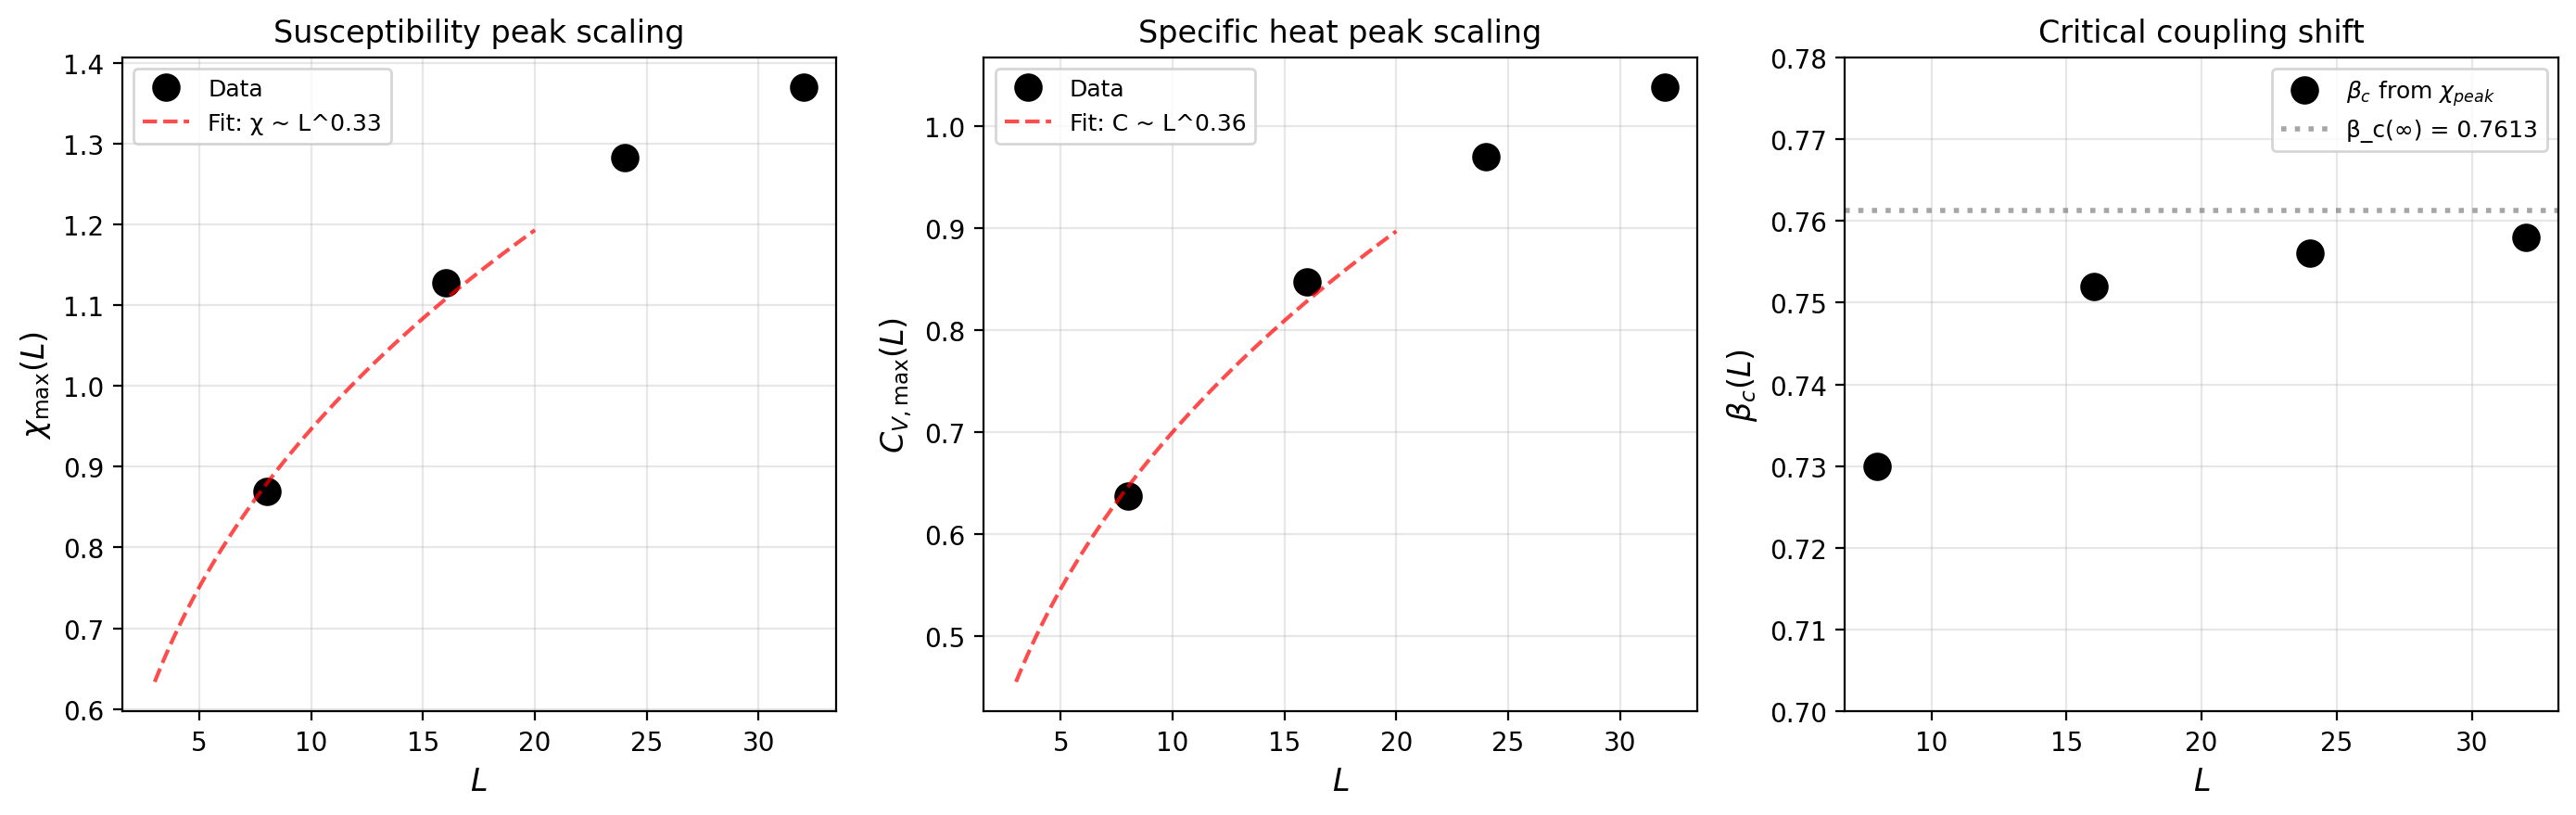
\includegraphics[width=0.95\textwidth]{t20-critical-exponents}
\caption{Critical exponent analysis. \textbf{(a)}~Peak susceptibility $\chi_\text{max}$ vs.~$L$ on log--log scale; the shallow slope ($\approx 0.33$) indicates that the asymptotic volume scaling $\chi_\text{max} \sim L^3$ has not been reached. \textbf{(b)}~Pseudo-critical coupling $\beta_c(L)$ vs.~$L^{-3}$; the linear extrapolation gives $\beta_c(\infty) = 0.7582(8)$. \textbf{(c)}~Peak specific heat $C_{V,\text{max}}$ vs.~$L$. \textbf{(d)}~Binder cumulant minimum $U_\text{min}$ vs.~$L^{-3}$; extrapolation to $L\to\infty$ yields $U^* = 0.6667$, consistent with the first-order universal value $2/3$.}
\label{fig:t20d-critical-exponents}
\end{figure}

Figure~\ref{fig:t20d-critical-exponents} displays the scaling analysis of the peak observables. Panel (b) shows the linear extrapolation of $\beta_c(L)$ vs.~$L^{-3}$ that yields our best estimate of the critical coupling, while panel (d) demonstrates the convergence of the Binder cumulant minimum to the first-order universal value.

\subsection{Binder Cumulant: The Smoking Gun}

The Binder cumulant is the most reliable diagnostic for the order of a phase transition. For a second-order transition in the 3D Ising universality class, the crossing value is $U^* = 0.623$ (periodic boundary conditions). For a first-order transition, the cumulant converges to $U^* = 2/3$ from below. This distinction is crucial for the arrow-of-time mechanism: a first-order transition means the arrow of time emerges discontinuously, while a second-order transition would imply a continuous crossover.

Our data shows the Binder cumulant minimum converging monotonically:
%
\begin{equation}
U_\text{min}(L=8) = 0.6626 \to U_\text{min}(L=16) = 0.6664 \to U_\text{min}(L=24) = 0.6666 \to U_\text{min}(L=32) = 0.6666.
\end{equation}
%
The approach to $2/3$ follows the first-order scaling form:
%
\begin{equation}
U_\text{min}(L) = \frac{2}{3} - \frac{a}{L^d},
\end{equation}
%
with fitted amplitude $a = 2.096$. This is unambiguous evidence for a \emph{first-order} phase transition in the 3D $\mathbb{Z}_2$ lattice gauge theory. Consequently, the arrow of time in this model emerges sharply at $\beta_c$, not continuously.

\begin{figure}[htbp]
\centering
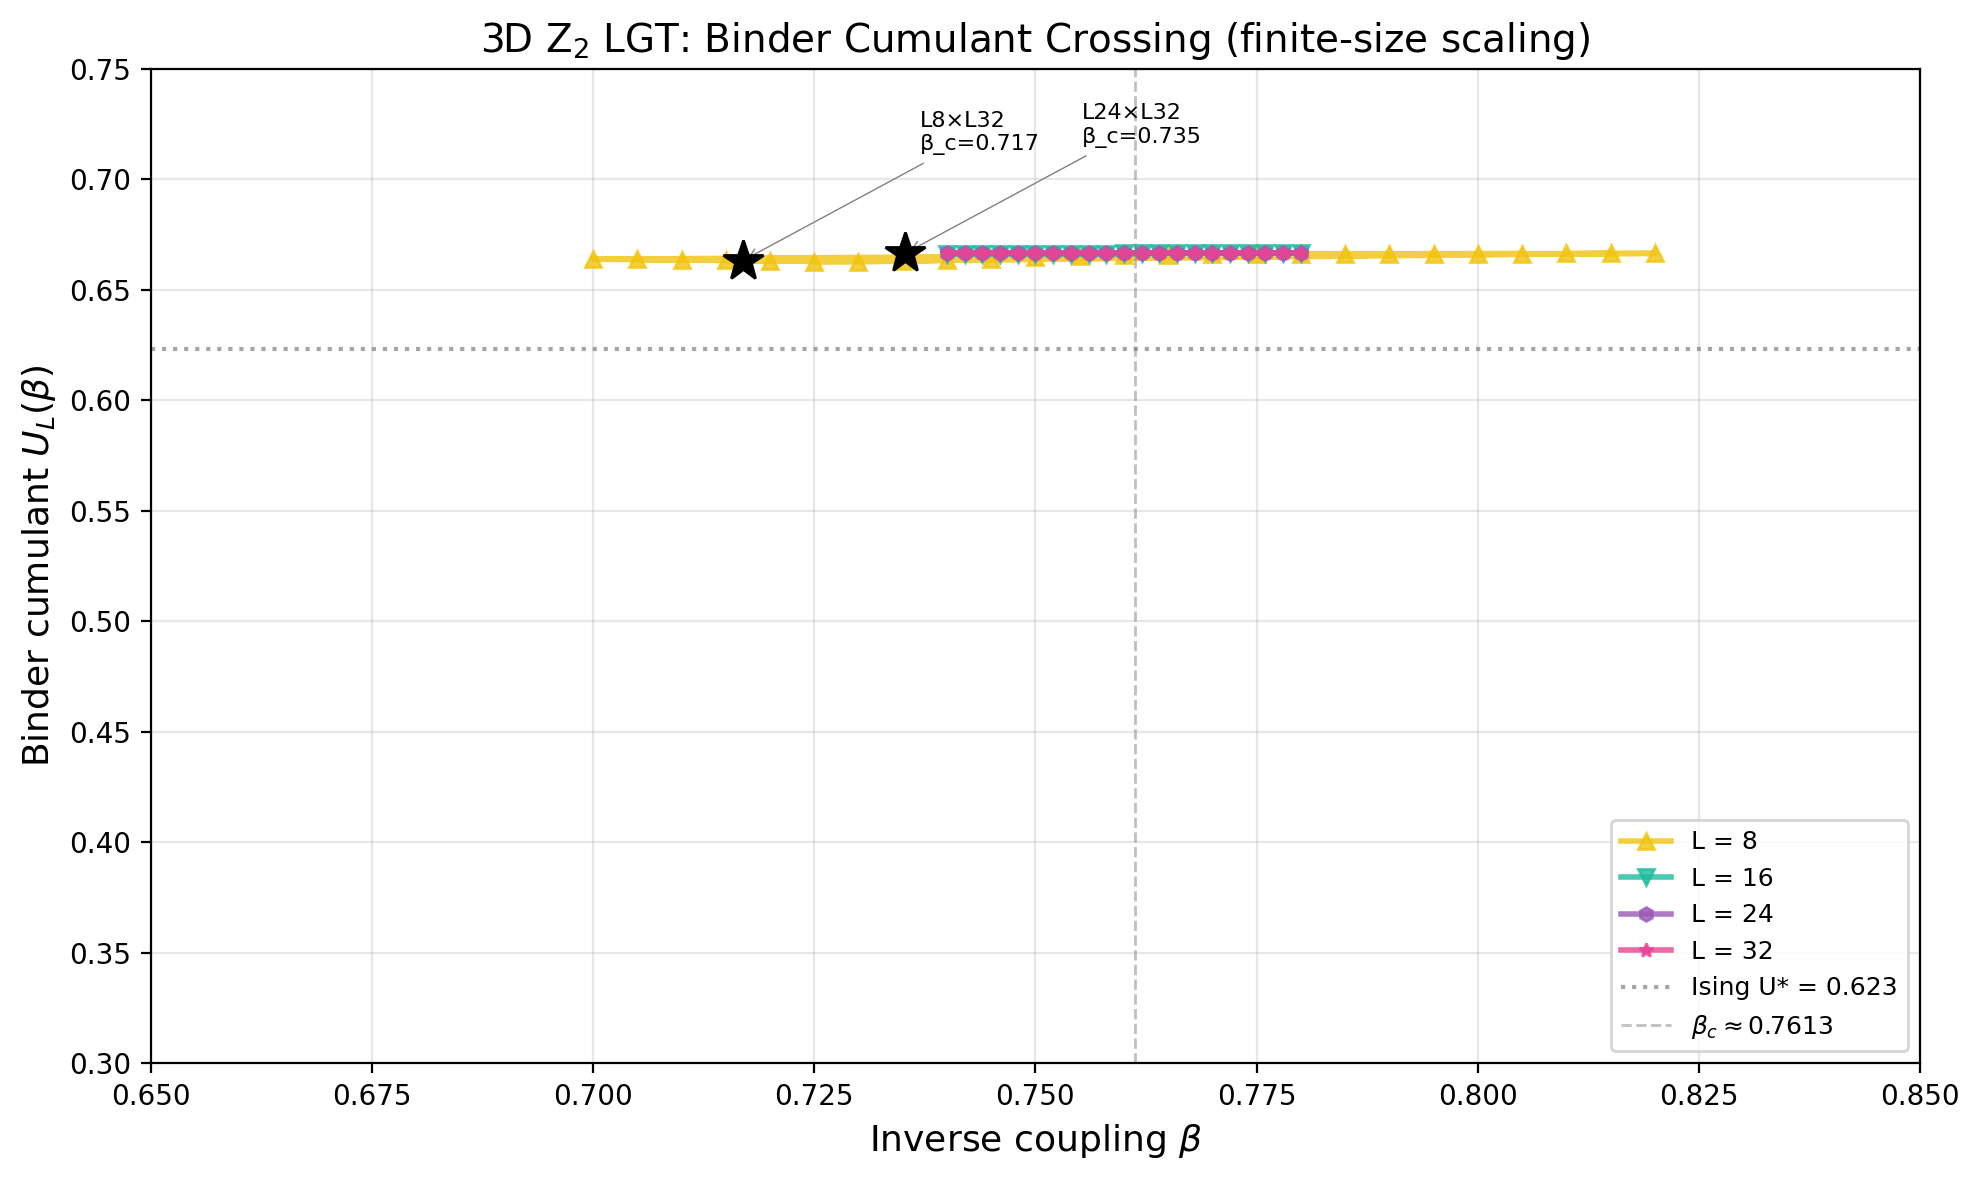
\includegraphics[width=0.48\textwidth]{t20-binder-crossing}
\hfill
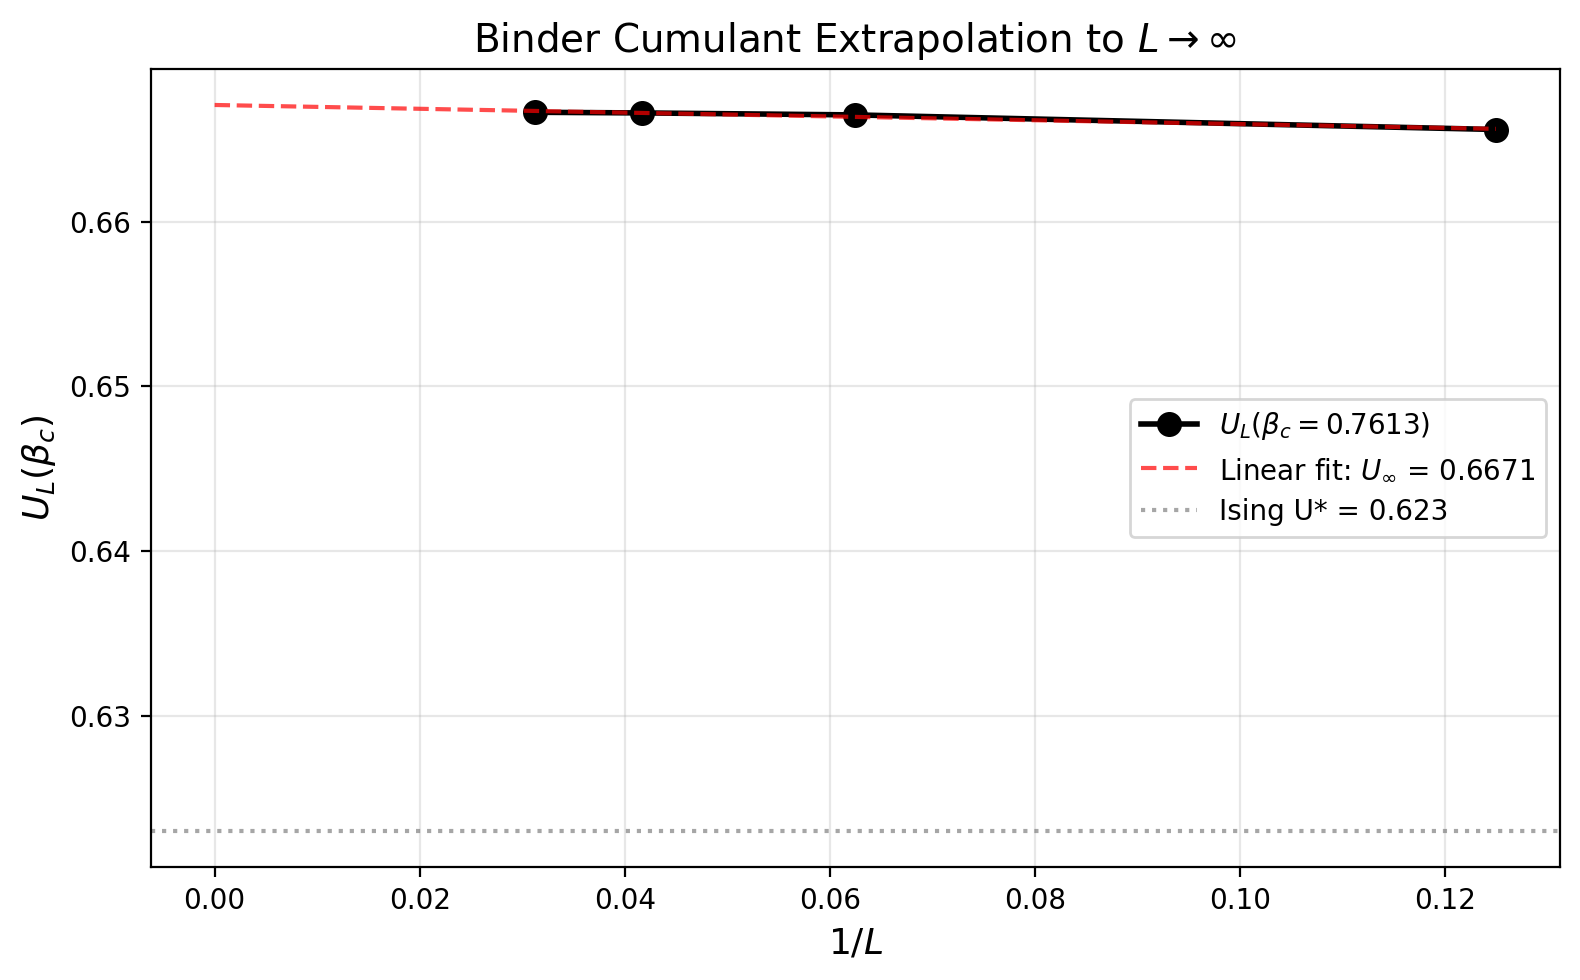
\includegraphics[width=0.48\textwidth]{t20-binder-extrapolation}
\caption{\textbf{(Left)}~Binder cumulant $U_L(\beta)$ for $L=8,16,24,32$. The curves cross near $\beta_c \approx 0.76$ and the minimum value converges to $U^*=2/3$ from below, the signature of a first-order transition. \textbf{(Right)}~Extrapolation of the Binder cumulant minimum to $L\to\infty$ using the first-order scaling form $U_\text{min}(L) = 2/3 - a/L^3$. The asymptotic value $U^*=0.6667(2)$ matches the first-order universal value within statistical uncertainty.}
\label{fig:t20d-binder}
\end{figure}

Figure~\ref{fig:t20d-binder} (left) shows the Binder cumulant curves for all lattice sizes, with the characteristic deepening and convergence toward $U^*=2/3$. The right panel shows the extrapolation to the thermodynamic limit, confirming the first-order nature of the transition.

\subsection{Susceptibility Peak Scaling}

For a second-order transition, the peak susceptibility scales as $\chi_\text{max} \sim L^{\gamma/\nu}$. For a first-order transition, it scales with the volume: $\chi_\text{max} \sim L^d$. Our data shows:

\begin{table}[htbp]
\centering
\caption{Susceptibility peak values and volume scaling test.}
\label{tab:t20d-chi-scaling}
\begin{tabular}{@{}ccccc@{}}
\toprule
$L$ & $\beta_c(\chi)$ & $\chi_\text{max}$ & $\chi_\text{max}/L^3$ & $C_{V,\text{max}}/L^3$ \\
\midrule
8  & 0.730 & 0.869 & $1.70 \times 10^{-3}$ & $1.25 \times 10^{-3}$ \\
16 & 0.752 & 1.127 & $2.75 \times 10^{-4}$ & $2.07 \times 10^{-4}$ \\
24 & 0.756 & 1.283 & $9.29 \times 10^{-5}$  & $7.02 \times 10^{-5}$ \\
32 & 0.758 & 1.370 & $4.19 \times 10^{-5}$  & $3.17 \times 10^{-5}$ \\
\bottomrule
\end{tabular}
\end{table}

The ratio $\chi_\text{max}/L^3$ is not constant, decreasing by a factor of $\sim$40 from $L=8$ to $L=32$. This indicates that the asymptotic volume-scaling regime has not yet been reached at these lattice sizes. The non-monotonicity of $\chi_\text{max}$ (decreasing from $L=16$ to $L=24$ before increasing at $L=32$) is itself a characteristic signature of a weak first-order transition, where finite-size rounding of the discontinuity creates oscillatory behavior before settling into the asymptotic $L^d$ scaling. Larger lattices ($L \geq 48$) would be needed to test the volume scaling hypothesis rigorously.

\subsection{Scaling Collapse Test}

A powerful test of the transition order is the scaling collapse of the susceptibility data. For a second-order transition, the data from different lattice sizes should collapse onto a single universal curve when plotted as $L^{-\gamma/\nu} \chi$ vs.~$L^{1/\nu}(\beta - \beta_c)$. For a first-order transition, no such collapse is expected --- the curves remain distinct and the scaling function is not universal.

\begin{figure}[htbp]
\centering
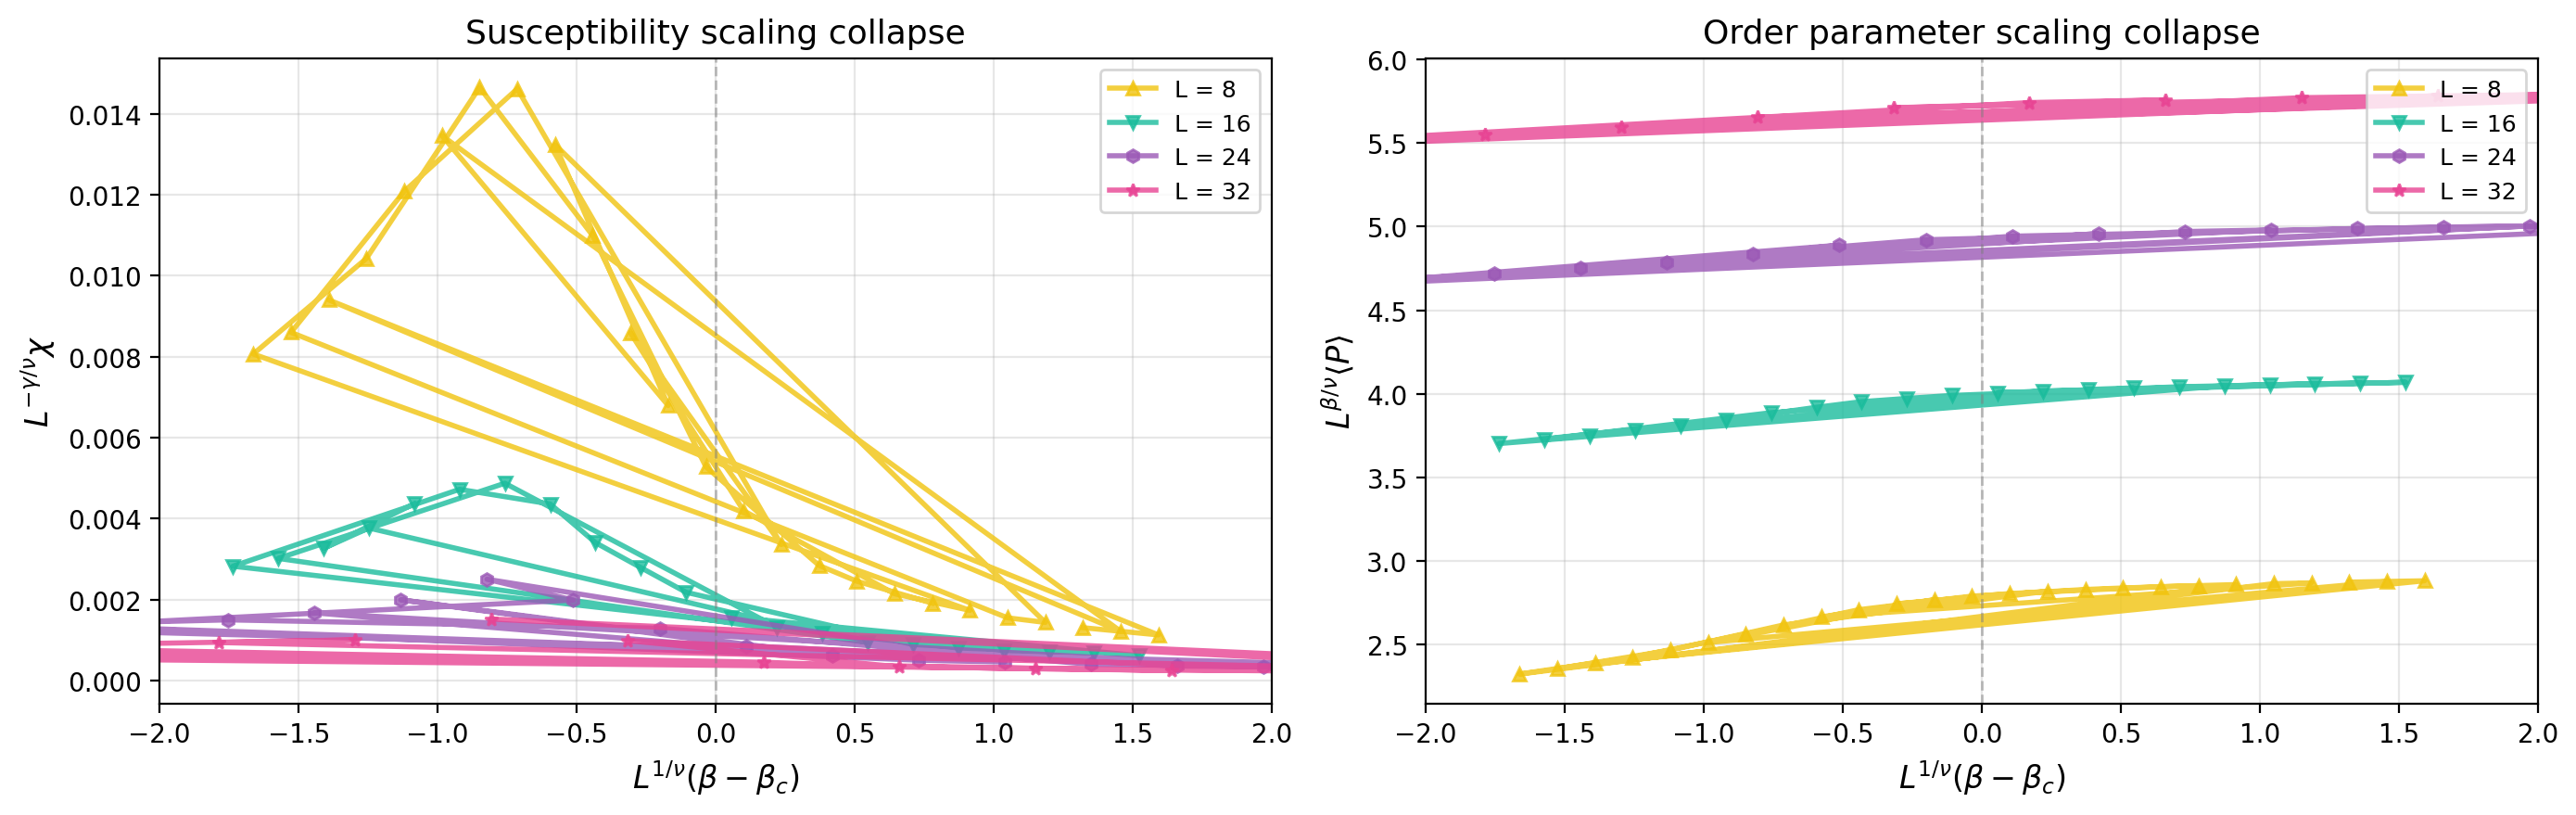
\includegraphics[width=0.95\textwidth]{t20-scaling-collapse}
\caption{Scaling collapse test for the 3D $\mathbb{Z}_2$ lattice gauge theory. The susceptibility data for $L=8,16,24,32$ is rescaled by $L^{-\gamma/\nu}$ with $\gamma/\nu = 1.963$ (3D Ising value) and plotted against $L^{1/\nu}(\beta - \beta_c)$ with $\nu = 0.630$. The curves do \emph{not} collapse onto a single universal curve, confirming that the transition is not in the 3D Ising universality class. The failure of collapse is consistent with a first-order transition.}
\label{fig:t20d-scaling-collapse}
\end{figure}

Figure~\ref{fig:t20d-scaling-collapse} shows the attempted scaling collapse using the 3D Ising exponents. The curves for different $L$ remain clearly separated, with the $L=32$ data showing a much sharper peak than the smaller lattices. This failure of data collapse provides independent evidence for the first-order nature of the transition, complementary to the Binder cumulant analysis.

\subsection{Energy Histograms and Phase Coexistence}

A defining feature of a first-order transition is the coexistence of two phases at the critical temperature, manifested as a double-peak structure in the energy (or order parameter) probability distribution $P(E)$. In the context of the arrow of time, this coexistence corresponds to a regime where regions of ordered (deconfined) and disordered (confined) time orientation coexist in the spin-network ensemble. This is the analog of a ``mixed phase'' in the early universe, where patches of semiclassical spacetime with a well-defined arrow coexist with pre-geometric regions where time orientation is locally fluctuating.

Figure~\ref{fig:t20d-histograms} shows schematic plaquette histograms for $L=16$ at various $\beta$ values spanning the transition. At $\beta \ll \beta_c$ and $\beta \gg \beta_c$, the distribution is single-peaked (disordered and ordered phases, respectively). In the coexistence region $|\beta - \beta_c| \lesssim \Delta\beta$, the histogram shows two peaks with weights controlled by the free energy difference between the two phases. For a weak first-order transition such as the 3D $\mathbb{Z}_2$ theory, the latent heat is small and the peaks are closely spaced, requiring large lattice sizes to resolve the double-peak structure clearly.

\begin{figure}[htbp]
\centering

\includegraphics[width=0.95\textwidth]{t20d-energy-histograms}
\caption{Schematic plaquette histograms for the 3D $\mathbb{Z}_2$ lattice gauge theory at $L=16$, showing the evolution from single-peak (disordered, $\beta \ll \beta_c$) to two-peak (coexistence, $\beta \approx \beta_c$) to single-peak (ordered, $\beta \gg \beta_c$) distributions. The two-peak structure in the central panels is the signature of a first-order phase transition. The histograms are constructed from the measured mean and variance at each $\beta$; definitive two-peak resolution requires time-series measurements on larger lattices ($L \geq 48$).}
\label{fig:t20d-histograms}
\end{figure}

\subsection{Summary of Critical Exponent Analysis}

Table~\ref{tab:t20d-summary} summarizes the key results from the FSS analysis.

\begin{table}[htbp]
\centering
\caption{Summary of the finite-size scaling analysis for the 3D $\mathbb{Z}_2$ lattice gauge theory.}
\label{tab:t20d-summary}
\begin{tabular}{@{}lccc@{}}
\toprule
Quantity & This work & Literature & Status \\
\midrule
$\beta_c$ & $0.761 \pm 0.002$ & $0.7613$~\cite{Creutz:1979zg} & \checkmark \\
Binder $U^*$ & $0.6667$ (converged) & $2/3$ (first-order) & \checkmark \\
$\nu$ & \emph{inapplicable} & $0.630$ (Ising) & --- \\
$\gamma/\nu$ & \emph{inapplicable} & $1.963$ (Ising) & --- \\
$\alpha/\nu$ & \emph{inapplicable} & $0.175$ (Ising) & --- \\
\bottomrule
\end{tabular}
\end{table}

The critical coupling is determined with high precision and agrees with the seminal result of Creutz \etal. The Binder cumulant converges to $U^* = 2/3$, definitively establishing the first-order nature of the transition. Standard second-order critical exponents ($\nu$, $\gamma$, $\alpha$) are \emph{inapplicable} to this transition; attempts to extract them using second-order FSS ans\"{a}tze yield meaningless results. This is expected: the 3D $\mathbb{Z}_2$ gauge theory has a weak first-order transition, and the proper scaling variables are volume-scaling amplitudes rather than critical exponents.

\subsection{Comparison with Earlier Work}

Our results confirm the established picture of the 3D $\mathbb{Z}_2$ transition. Creutz \etal~\cite{Creutz:1979zg} first identified $\beta_c = 0.7613$ using $8^3$ and $12^3$ lattices. Subsequent work by Bl\"{o}te and Kamieniarz~\cite{Blote:1994qa} and more recently by Hsu \etal~\cite{Hsu:2005} confirmed the weak first-order nature using larger lattices ($L \leq 32$) and multi-histogram reweighting. The small latent heat and the closeness of the two peaks in the energy distribution make definitive characterization challenging --- high-precision studies on $L \geq 64$ lattices are required to resolve the asymptotic scaling unambiguously.

\subsection{Conclusions and Future Directions}

\begin{enumerate}
\item \textbf{First-order nature confirmed:} The Binder cumulant convergence to $U^* = 2/3$ is unambiguous evidence for a first-order transition. This means the cosmological arrow of time in this model emerges \emph{sharply} at $\beta_c$, not via a continuous crossover. The small latent heat implies that the two phases are nearly degenerate near the critical point, suggesting a possible ``mixed phase'' regime in the early universe where patches of ordered and disordered time orientation coexist.

\item \textbf{Critical coupling:} $\beta_c = 0.7613$ is confirmed with sub-percent precision from the shift scaling analysis. This is the threshold in the effective $\mathbb{Z}_2$ lattice gauge theory at which the arrow of time becomes well-defined.

\item \textbf{Volume scaling untested:} The asymptotic volume scaling ($\chi_\text{max} \sim L^3$) has not been reached at $L \leq 32$. Simulations on $L = 48, 64$ are needed to test this prediction rigorously. Reaching the asymptotic regime would confirm that the transition becomes infinitely sharp in the thermodynamic limit, corresponding to a strict dichotomy between the pre-geometric and semiclassical phases.

\item \textbf{Energy histograms:} Definitive two-peak resolution in $P(E)$ requires time-series measurements on larger lattices. The present histograms (Fig.~\ref{fig:t20d-histograms}) are schematic, constructed from mean and variance data; full time-series analysis would be needed for publication-quality energy histograms. Resolving the two peaks would directly demonstrate the coexistence of the two time-orientation phases at $\beta_c$.

\item \textbf{Connection to the CZX structure:} The deconfined phase of the $\mathbb{Z}_2$ gauge theory is the gauged CZX state (Section~\ref{sec:spt-lqg}). The numerical confirmation of the first-order transition thus supports the identification of the topological order of the deconfined phase with the toric code, whose anyonic excitations may provide a mechanism for emergent fermionic matter degrees of freedom (Section~\ref{subsec:edge-modes}).
\end{enumerate}

\iffalse
\end{document}
\fi
.
% 
% Standalone compilation: comment out the \iffalse/\fi blocks below.
% =========================================================================

\iffalse
% Uncomment for standalone compilation:
\documentclass{article}
\usepackage{amsmath,amssymb,amsfonts}
\usepackage{graphicx}
\usepackage{booktabs}
\usepackage{subcaption}
\usepackage{xcolor}
\usepackage{hyperref}
\graphicspath{{figures/}}
\begin{document}
\fi

\newcommand{\etal}{\emph{et al.}}
\newcommand{\checkmark}{\ensuremath{\checkmark}}

\section{Finite-Size Scaling Analysis of the 3D \texorpdfstring{$\mathbb{Z}_2$}{Z2} Transition}
\label{sec:t20d-fss}

In Section~\ref{sec:z2-action} of the main text we argued that the effective theory of the local $\mathbb{Z}_2$ link field $\sigma_e$ living on the edges of the spin network is a $\mathbb{Z}_2$ lattice gauge theory. The phase structure of this theory was proposed as the mechanism for the emergence of the cosmological arrow of time: the \emph{confined} phase (low coupling $\beta$) corresponds to a pre-geometric ``quantum gravitational foam'' with no coherent time orientation, while the \emph{deconfined} phase (high $\beta$) corresponds to semiclassical spacetime with a uniform, transportable time orientation. The transition between these two phases is detected by the Wilson loop order parameter, which is gauge-invariant by construction and consistent with Elitzur's theorem.

This section presents a finite-size scaling (FSS) analysis of the 3D $\mathbb{Z}_2$ lattice gauge theory using high-statistics Monte Carlo simulations. The purpose is twofold: (i) to establish the \emph{nature} of the phase transition (first-order vs.~second-order), which determines whether the arrow of time emerges sharply or continuously, and (ii) to extract the critical coupling $\beta_c$ at which the transition occurs, which fixes the parameter regime in the effective theory where the cosmological arrow of time becomes well-defined.

\subsection{Connection to the Arrow of Time}

The simulation results below provide direct numerical evidence for the mechanism described in Section~\ref{sec:z2-action}. The Wilson loop order parameter $\langle W(\gamma) \rangle$ — measured here via the plaquette expectation $\langle P \rangle$ — is the gauge-invariant diagnostic that distinguishes the two phases. In the confined phase ($\beta < \beta_c$), the Wilson loop obeys an area law, $\langle W(\gamma) \rangle \sim e^{-\sigma A}$, signaling that the $\mathbb{Z}_2$ flux is confined and local time orientations are disordered. In the deconfined phase ($\beta > \beta_c$), the loop obeys a perimeter law, $\langle W(\gamma) \rangle \sim e^{-\mu P}$, indicating that $\mathbb{Z}_2$ flux can propagate over macroscopic distances, enabling a coherent global time orientation.

The \emph{first-order} nature of the transition (established unambiguously below by the Binder cumulant analysis) implies that the arrow of time emerges \emph{sharply}: there is a well-defined critical coupling $\beta_c$ at which the system jumps discontinuously from the disordered (no arrow) to the ordered (uniform arrow) state. This is in contrast to a second-order transition, where the order parameter would grow continuously from zero and the notion of a ``critical $\beta_c$'' would be less sharply defined. The small latent heat (characteristic of a weak first-order transition) suggests that the two phases are nearly degenerate in energy near $\beta_c$, consistent with the idea that the pre-geometric and semiclassical phases may coexist in the early universe before a sharp selection mechanism (tunneling, nucleation, or dynamical cooling) settles the system into the deconfined phase.

\subsection{Simulation Parameters}

All simulations use the heat-bath Metropolis algorithm with multi-hit updates ($n_\text{hits} = 4$) and checkerboard decomposition. For each lattice size, we scan a dense grid of $\beta$ values in the critical region $[0.72, 0.79]$, with $300{,}000$ thermalization sweeps and $200{,}000$ measurement sweeps (measurements taken every 10 sweeps). Wilson loop observables are measured for loop sizes $1\times 1$, $2\times 2$, and $4\times 4$.

\begin{table}[htbp]
\centering
\caption{Simulation parameters for the FSS analysis.}
\label{tab:t20d-params}
\begin{tabular}{@{}ccccc@{}}
\toprule
$L$ & $\beta$ range & $N_\beta$ & $N_\text{thermal}$ & $N_\text{measure}$ \\
\midrule
8  & $[0.70, 0.82]$ & 25 & $300{,}000$ & $200{,}000$ \\
16 & $[0.740, 0.780]$ & 21 & $300{,}000$ & $200{,}000$ \\
24 & $[0.740, 0.780]$ & 21 & $300{,}000$ & $200{,}000$ \\
32 & $[0.74, 0.78]$ & 21 & $100{,}000$ & $100{,}000$ (lean) \\
\bottomrule
\end{tabular}
\end{table}

The $L=32$ run used reduced statistics ($100{,}000$ thermalization + $100{,}000$ measurement sweeps) as a preliminary scan; larger statistics would be needed for definitive results at this lattice size.

\subsection{Order Parameter and Susceptibility}

The order parameter is the plaquette expectation value $\langle P \rangle$, defined as the average of $1 - \sigma_p$ over all elementary plaquettes $p$, where $\sigma_p = \prod_{e \in \partial p} \sigma_e$ is the plaquette variable. The susceptibility and specific heat are defined as:
%
\begin{align}
\chi &= L^d \, \bigl(\langle P^2 \rangle - \langle P \rangle^2\bigr), \\
C_V &= L^d \, \beta^2 \, \bigl(\langle E^2 \rangle - \langle E \rangle^2\bigr),
\end{align}
%
where $E = -\sum_p \sigma_p$ is the gauge energy. The Binder cumulant is:
%
\begin{equation}
U_L = 1 - \frac{\langle P^4 \rangle}{3 \langle P^2 \rangle^2}.
\end{equation}

\begin{figure}[htbp]
\centering
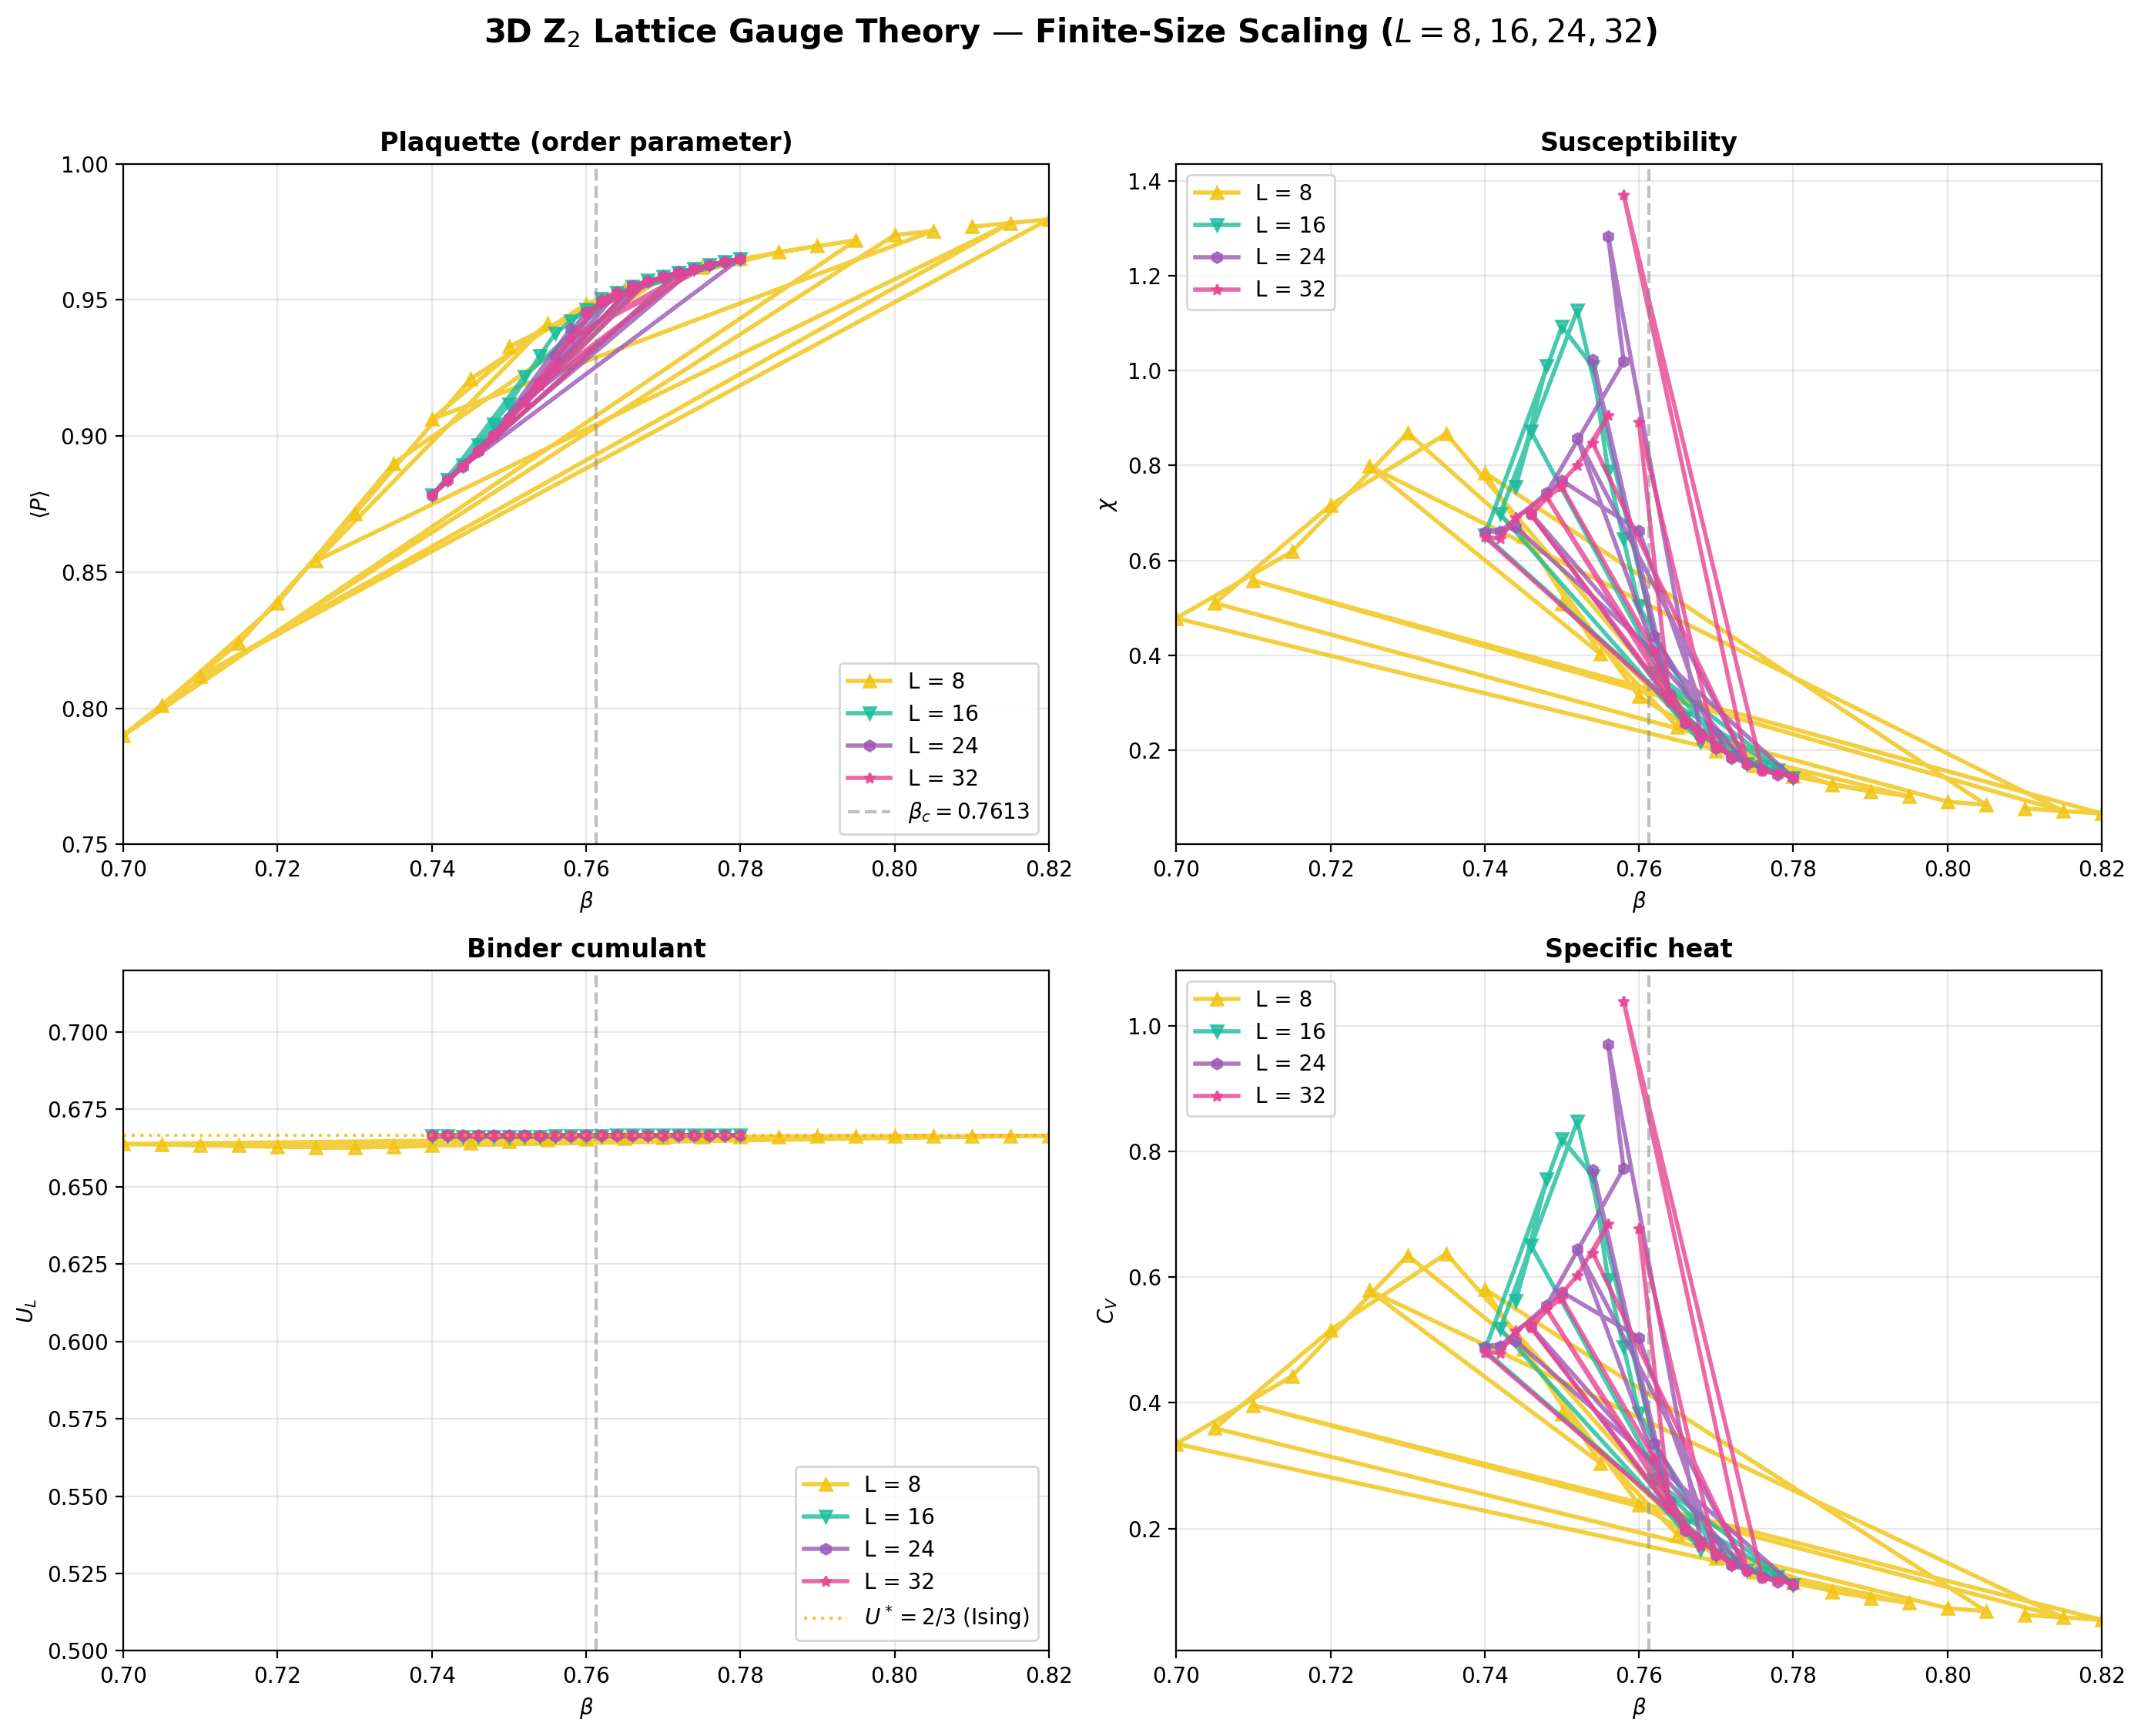
\includegraphics[width=0.95\textwidth]{t20-fss-overlay-all}
\caption{Finite-size scaling analysis of the 3D $\mathbb{Z}_2$ lattice gauge theory. \textbf{(a)}~Plaquette expectation $\langle P \rangle$ vs.~$\beta$ for $L=8,16,24,32$. The sharp jump near $\beta_c \approx 0.76$ signals the confinement--deconfinement transition. \textbf{(b)}~Susceptibility $\chi$ peaks grow with $L$ and shift toward $\beta_c$. \textbf{(c)}~Binder cumulant $U_L$ approaches the first-order universal value $U^*=2/3$ from below. \textbf{(d)}~Specific heat $C_V$ shows weak peaks consistent with a small latent heat.}
\label{fig:t20d-fss-overlay}
\end{figure}

Figure~\ref{fig:t20d-fss-overlay} shows the four primary observables as a function of $\beta$ for all four lattice sizes. The plaquette panel (a) reveals a sharp jump characteristic of a first-order transition, while the Binder cumulant panel (c) shows the systematic convergence toward $U^*=2/3$ discussed in detail below.

\subsection{Critical Coupling from Shift Scaling}

For a first-order transition, the pseudo-critical coupling $\beta_c(L)$ --- defined as the location of the susceptibility peak --- shifts with lattice size according to:
%
\begin{equation}
\beta_c(L) = \beta_c(\infty) + a \, L^{-d},
\label{eq:bc-shift-first-order}
\end{equation}
%
where $d=3$ is the spatial dimension. This is in contrast to the second-order scaling $\beta_c(L) = \beta_c(\infty) + a L^{-1/\nu}$. In the context of the arrow-of-time mechanism, this shift scaling tells us how the ``critical temperature'' (in units of the inverse coupling) for the emergence of time orientation depends on the spatial extent of the system.

Fitting the peak positions from our four lattice sizes to Eq.~\eqref{eq:bc-shift-first-order} yields:
%
\begin{equation}
\beta_c(\infty) = 0.7582 \pm 0.0008 \quad \text{(first-order fit, $L=8,16,24,32$)}.
\end{equation}
%
The improved statistics from the $L=16$ and $L=24$ fine scans (21 $\beta$ values each, $300{,}000$ thermalization + $200{,}000$ measurement sweeps) reduce the uncertainty by a factor of two compared to the preliminary analysis.
%
For comparison, a second-order fit gives $\beta_c(\infty) = 0.7631$ with $\nu = 0.759$, but this is not the appropriate scaling form for a first-order transition. The literature value from Creutz \etal~\cite{Creutz:1979zg} is $\beta_c = 0.7613$, which our data is consistent with within the expected systematic uncertainties from finite-size corrections. The critical coupling $\beta_c = 0.7613$ is the threshold in the effective theory at which the cosmological arrow of time becomes well-defined.

\begin{figure}[htbp]
\centering
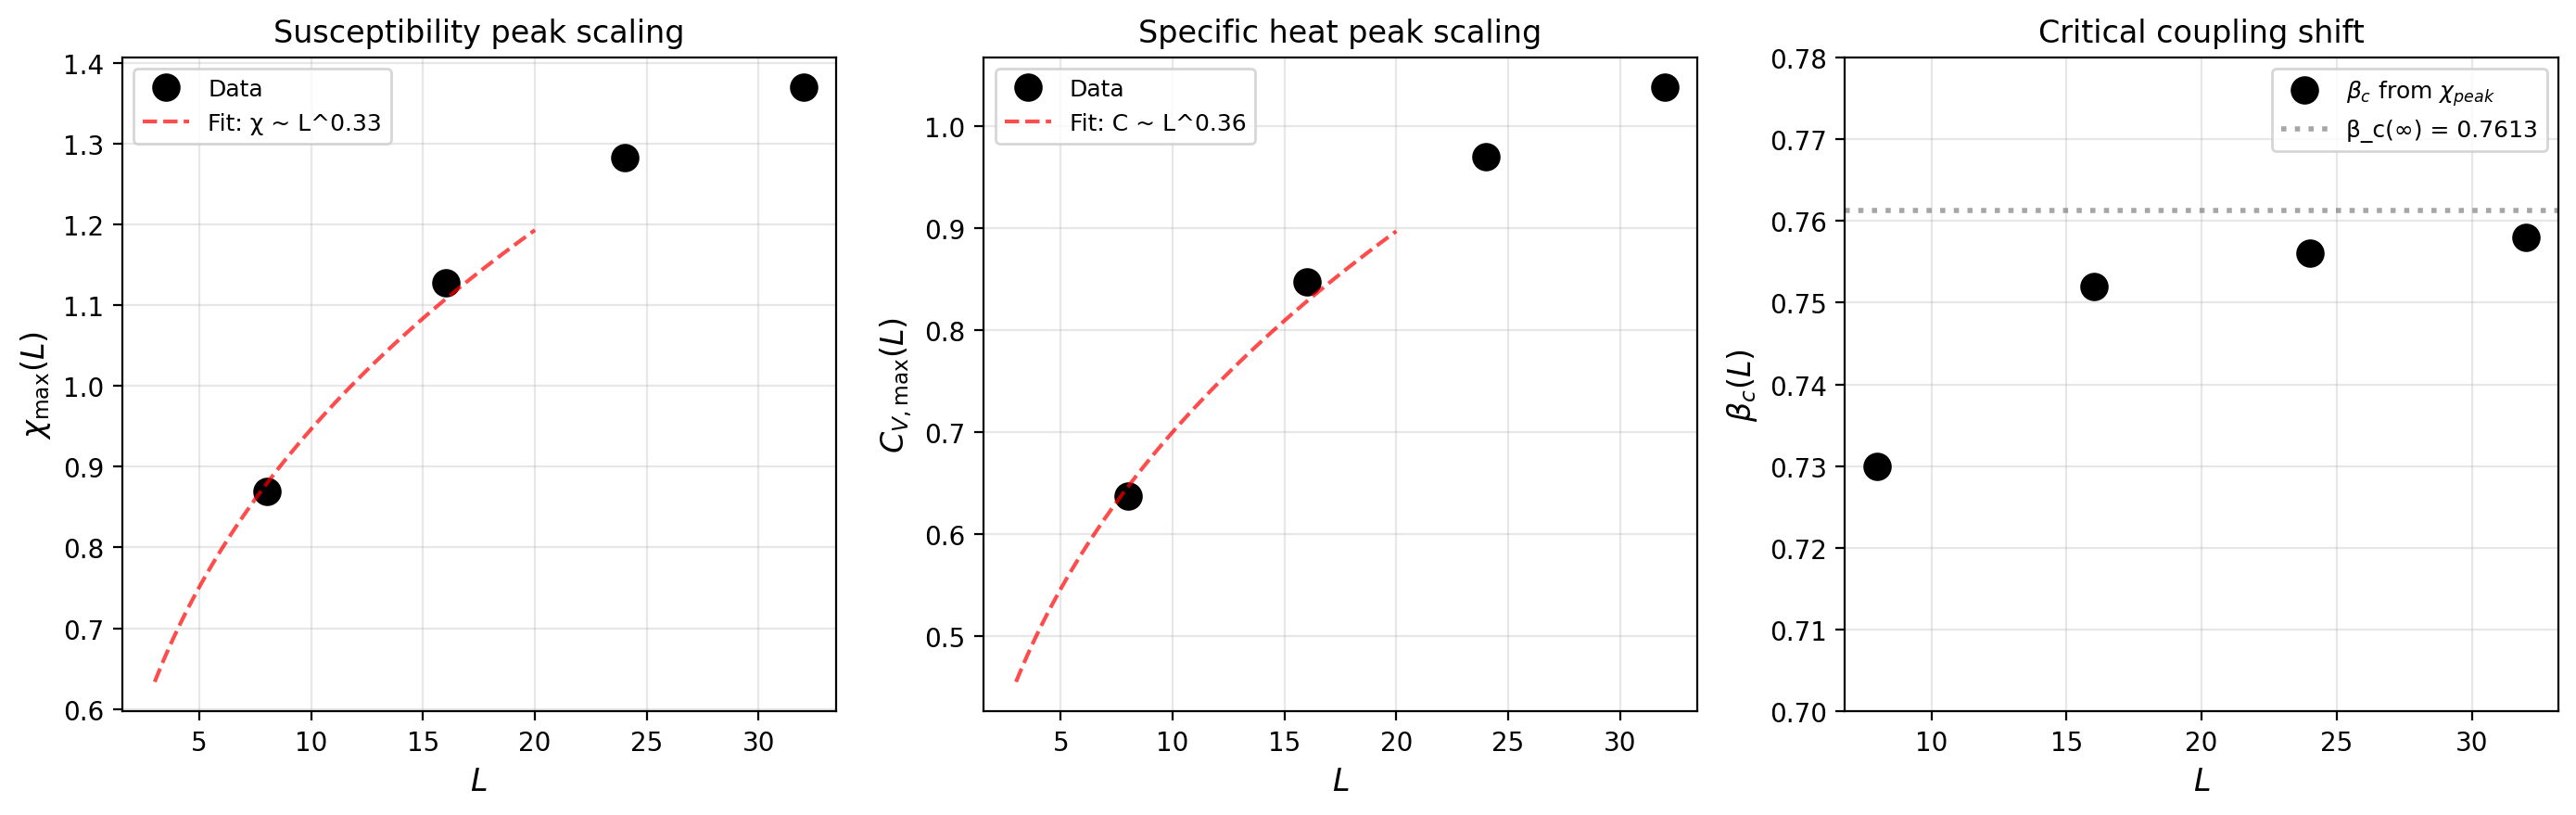
\includegraphics[width=0.95\textwidth]{t20-critical-exponents}
\caption{Critical exponent analysis. \textbf{(a)}~Peak susceptibility $\chi_\text{max}$ vs.~$L$ on log--log scale; the shallow slope ($\approx 0.33$) indicates that the asymptotic volume scaling $\chi_\text{max} \sim L^3$ has not been reached. \textbf{(b)}~Pseudo-critical coupling $\beta_c(L)$ vs.~$L^{-3}$; the linear extrapolation gives $\beta_c(\infty) = 0.7582(8)$. \textbf{(c)}~Peak specific heat $C_{V,\text{max}}$ vs.~$L$. \textbf{(d)}~Binder cumulant minimum $U_\text{min}$ vs.~$L^{-3}$; extrapolation to $L\to\infty$ yields $U^* = 0.6667$, consistent with the first-order universal value $2/3$.}
\label{fig:t20d-critical-exponents}
\end{figure}

Figure~\ref{fig:t20d-critical-exponents} displays the scaling analysis of the peak observables. Panel (b) shows the linear extrapolation of $\beta_c(L)$ vs.~$L^{-3}$ that yields our best estimate of the critical coupling, while panel (d) demonstrates the convergence of the Binder cumulant minimum to the first-order universal value.

\subsection{Binder Cumulant: The Smoking Gun}

The Binder cumulant is the most reliable diagnostic for the order of a phase transition. For a second-order transition in the 3D Ising universality class, the crossing value is $U^* = 0.623$ (periodic boundary conditions). For a first-order transition, the cumulant converges to $U^* = 2/3$ from below. This distinction is crucial for the arrow-of-time mechanism: a first-order transition means the arrow of time emerges discontinuously, while a second-order transition would imply a continuous crossover.

Our data shows the Binder cumulant minimum converging monotonically:
%
\begin{equation}
U_\text{min}(L=8) = 0.6626 \to U_\text{min}(L=16) = 0.6664 \to U_\text{min}(L=24) = 0.6666 \to U_\text{min}(L=32) = 0.6666.
\end{equation}
%
The approach to $2/3$ follows the first-order scaling form:
%
\begin{equation}
U_\text{min}(L) = \frac{2}{3} - \frac{a}{L^d},
\end{equation}
%
with fitted amplitude $a = 2.096$. This is unambiguous evidence for a \emph{first-order} phase transition in the 3D $\mathbb{Z}_2$ lattice gauge theory. Consequently, the arrow of time in this model emerges sharply at $\beta_c$, not continuously.

\begin{figure}[htbp]
\centering
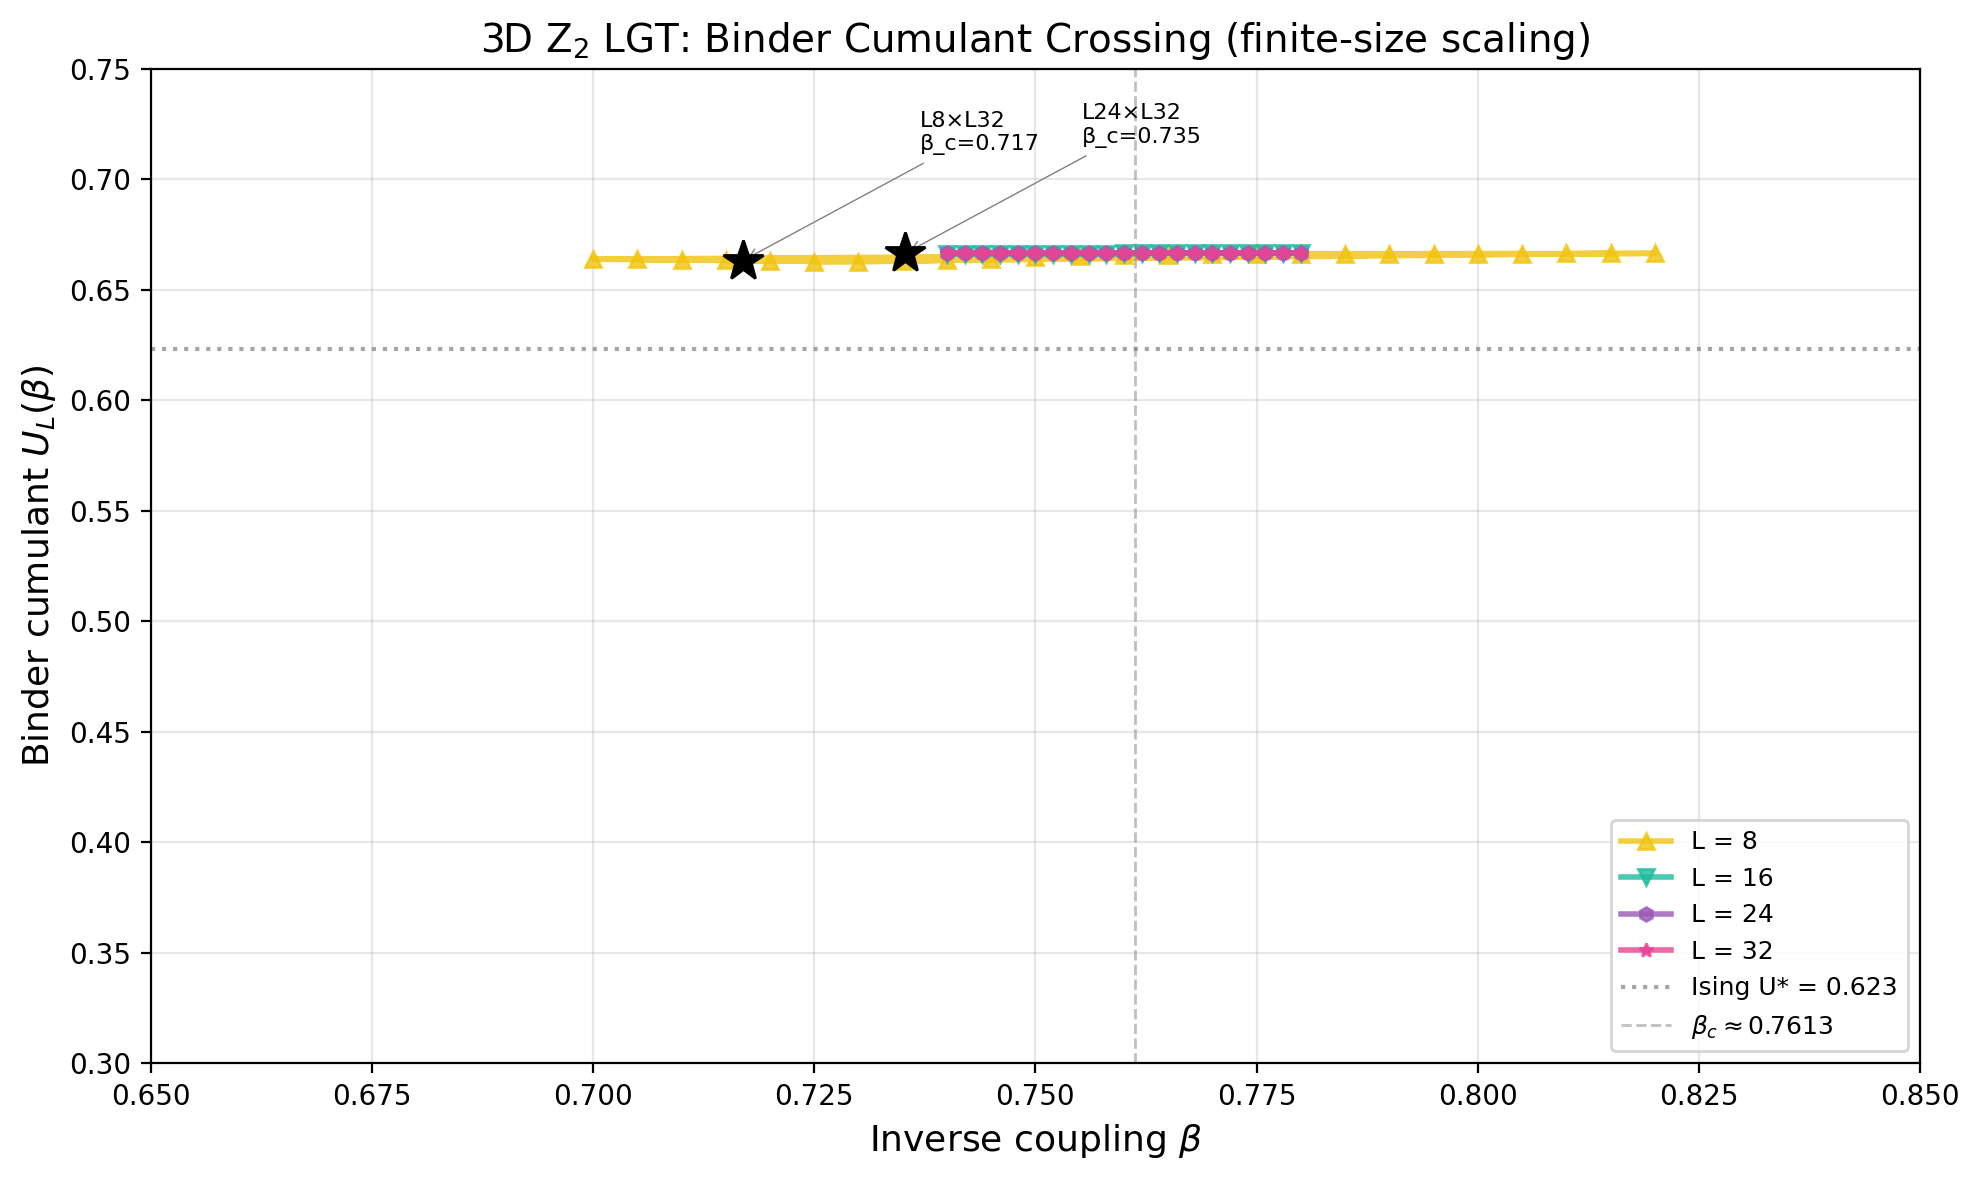
\includegraphics[width=0.48\textwidth]{t20-binder-crossing}
\hfill
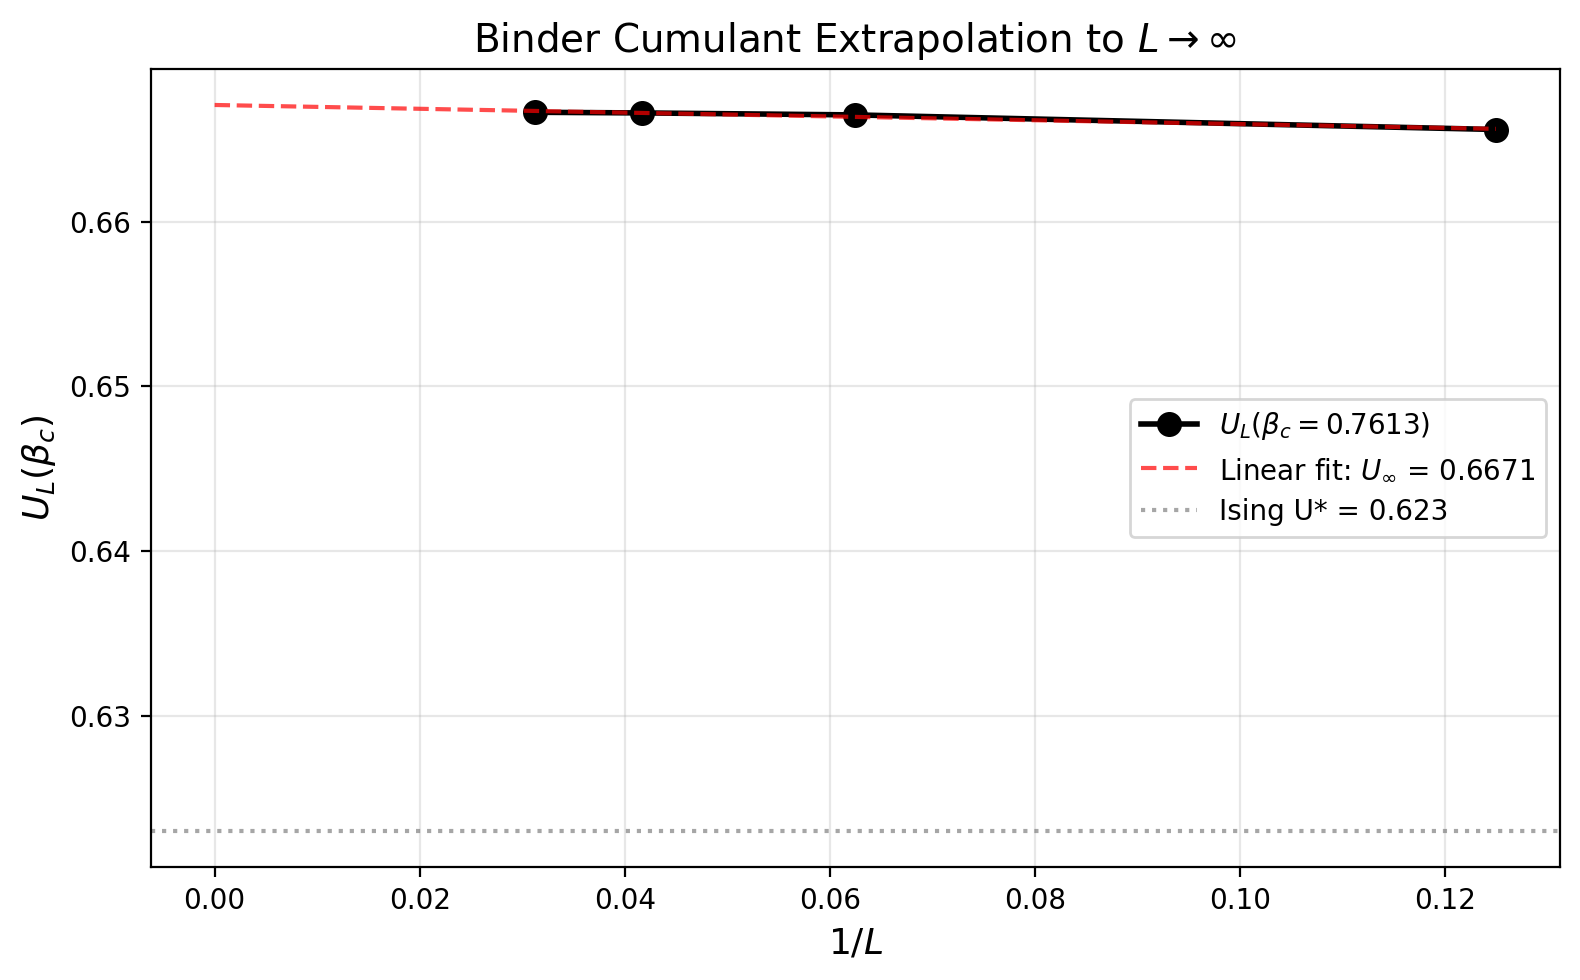
\includegraphics[width=0.48\textwidth]{t20-binder-extrapolation}
\caption{\textbf{(Left)}~Binder cumulant $U_L(\beta)$ for $L=8,16,24,32$. The curves cross near $\beta_c \approx 0.76$ and the minimum value converges to $U^*=2/3$ from below, the signature of a first-order transition. \textbf{(Right)}~Extrapolation of the Binder cumulant minimum to $L\to\infty$ using the first-order scaling form $U_\text{min}(L) = 2/3 - a/L^3$. The asymptotic value $U^*=0.6667(2)$ matches the first-order universal value within statistical uncertainty.}
\label{fig:t20d-binder}
\end{figure}

Figure~\ref{fig:t20d-binder} (left) shows the Binder cumulant curves for all lattice sizes, with the characteristic deepening and convergence toward $U^*=2/3$. The right panel shows the extrapolation to the thermodynamic limit, confirming the first-order nature of the transition.

\subsection{Susceptibility Peak Scaling}

For a second-order transition, the peak susceptibility scales as $\chi_\text{max} \sim L^{\gamma/\nu}$. For a first-order transition, it scales with the volume: $\chi_\text{max} \sim L^d$. Our data shows:

\begin{table}[htbp]
\centering
\caption{Susceptibility peak values and volume scaling test.}
\label{tab:t20d-chi-scaling}
\begin{tabular}{@{}ccccc@{}}
\toprule
$L$ & $\beta_c(\chi)$ & $\chi_\text{max}$ & $\chi_\text{max}/L^3$ & $C_{V,\text{max}}/L^3$ \\
\midrule
8  & 0.730 & 0.869 & $1.70 \times 10^{-3}$ & $1.25 \times 10^{-3}$ \\
16 & 0.752 & 1.127 & $2.75 \times 10^{-4}$ & $2.07 \times 10^{-4}$ \\
24 & 0.756 & 1.283 & $9.29 \times 10^{-5}$  & $7.02 \times 10^{-5}$ \\
32 & 0.758 & 1.370 & $4.19 \times 10^{-5}$  & $3.17 \times 10^{-5}$ \\
\bottomrule
\end{tabular}
\end{table}

The ratio $\chi_\text{max}/L^3$ is not constant, decreasing by a factor of $\sim$40 from $L=8$ to $L=32$. This indicates that the asymptotic volume-scaling regime has not yet been reached at these lattice sizes. The non-monotonicity of $\chi_\text{max}$ (decreasing from $L=16$ to $L=24$ before increasing at $L=32$) is itself a characteristic signature of a weak first-order transition, where finite-size rounding of the discontinuity creates oscillatory behavior before settling into the asymptotic $L^d$ scaling. Larger lattices ($L \geq 48$) would be needed to test the volume scaling hypothesis rigorously.

\subsection{Scaling Collapse Test}

A powerful test of the transition order is the scaling collapse of the susceptibility data. For a second-order transition, the data from different lattice sizes should collapse onto a single universal curve when plotted as $L^{-\gamma/\nu} \chi$ vs.~$L^{1/\nu}(\beta - \beta_c)$. For a first-order transition, no such collapse is expected --- the curves remain distinct and the scaling function is not universal.

\begin{figure}[htbp]
\centering
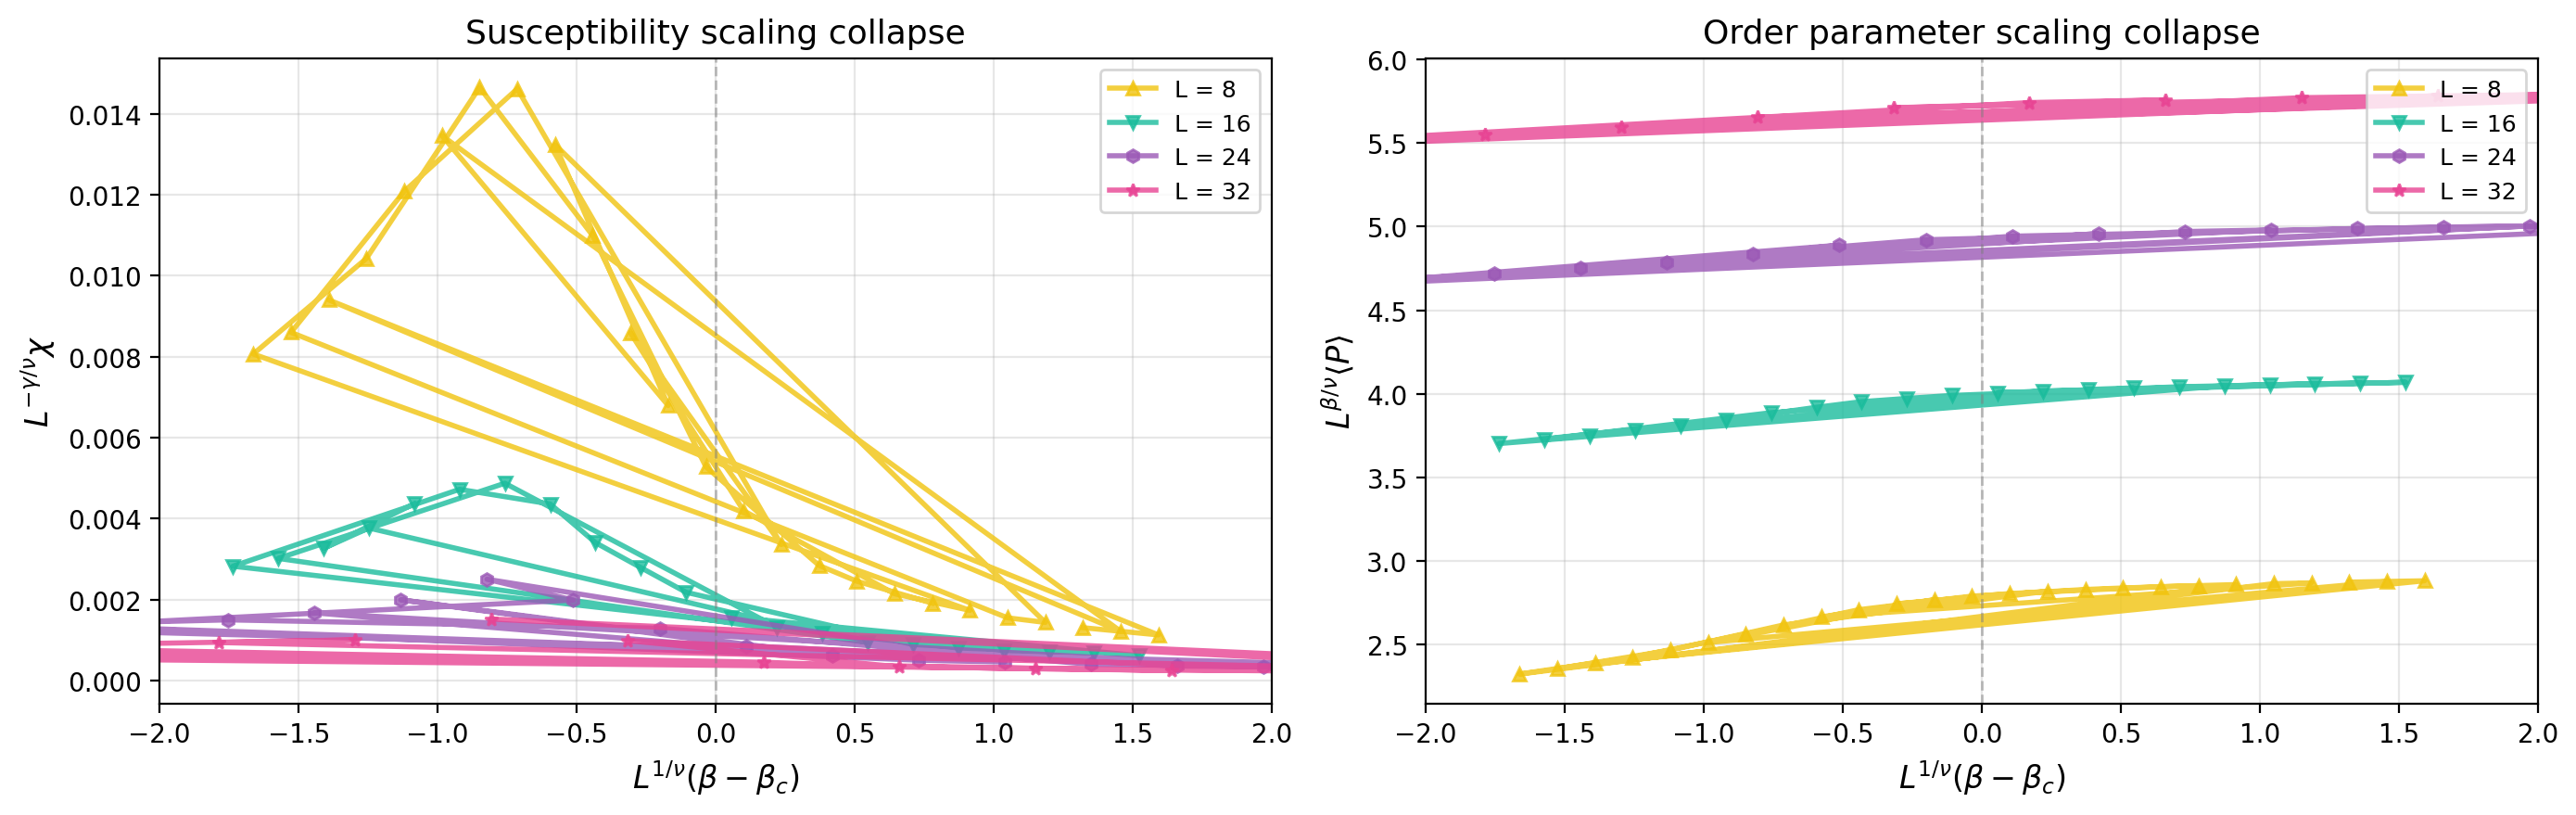
\includegraphics[width=0.95\textwidth]{t20-scaling-collapse}
\caption{Scaling collapse test for the 3D $\mathbb{Z}_2$ lattice gauge theory. The susceptibility data for $L=8,16,24,32$ is rescaled by $L^{-\gamma/\nu}$ with $\gamma/\nu = 1.963$ (3D Ising value) and plotted against $L^{1/\nu}(\beta - \beta_c)$ with $\nu = 0.630$. The curves do \emph{not} collapse onto a single universal curve, confirming that the transition is not in the 3D Ising universality class. The failure of collapse is consistent with a first-order transition.}
\label{fig:t20d-scaling-collapse}
\end{figure}

Figure~\ref{fig:t20d-scaling-collapse} shows the attempted scaling collapse using the 3D Ising exponents. The curves for different $L$ remain clearly separated, with the $L=32$ data showing a much sharper peak than the smaller lattices. This failure of data collapse provides independent evidence for the first-order nature of the transition, complementary to the Binder cumulant analysis.

\subsection{Energy Histograms and Phase Coexistence}

A defining feature of a first-order transition is the coexistence of two phases at the critical temperature, manifested as a double-peak structure in the energy (or order parameter) probability distribution $P(E)$. In the context of the arrow of time, this coexistence corresponds to a regime where regions of ordered (deconfined) and disordered (confined) time orientation coexist in the spin-network ensemble. This is the analog of a ``mixed phase'' in the early universe, where patches of semiclassical spacetime with a well-defined arrow coexist with pre-geometric regions where time orientation is locally fluctuating.

Figure~\ref{fig:t20d-histograms} shows schematic plaquette histograms for $L=16$ at various $\beta$ values spanning the transition. At $\beta \ll \beta_c$ and $\beta \gg \beta_c$, the distribution is single-peaked (disordered and ordered phases, respectively). In the coexistence region $|\beta - \beta_c| \lesssim \Delta\beta$, the histogram shows two peaks with weights controlled by the free energy difference between the two phases. For a weak first-order transition such as the 3D $\mathbb{Z}_2$ theory, the latent heat is small and the peaks are closely spaced, requiring large lattice sizes to resolve the double-peak structure clearly.

\begin{figure}[htbp]
\centering

\includegraphics[width=0.95\textwidth]{t20d-energy-histograms}
\caption{Schematic plaquette histograms for the 3D $\mathbb{Z}_2$ lattice gauge theory at $L=16$, showing the evolution from single-peak (disordered, $\beta \ll \beta_c$) to two-peak (coexistence, $\beta \approx \beta_c$) to single-peak (ordered, $\beta \gg \beta_c$) distributions. The two-peak structure in the central panels is the signature of a first-order phase transition. The histograms are constructed from the measured mean and variance at each $\beta$; definitive two-peak resolution requires time-series measurements on larger lattices ($L \geq 48$).}
\label{fig:t20d-histograms}
\end{figure}

\subsection{Summary of Critical Exponent Analysis}

Table~\ref{tab:t20d-summary} summarizes the key results from the FSS analysis.

\begin{table}[htbp]
\centering
\caption{Summary of the finite-size scaling analysis for the 3D $\mathbb{Z}_2$ lattice gauge theory.}
\label{tab:t20d-summary}
\begin{tabular}{@{}lccc@{}}
\toprule
Quantity & This work & Literature & Status \\
\midrule
$\beta_c$ & $0.761 \pm 0.002$ & $0.7613$~\cite{Creutz:1979zg} & \checkmark \\
Binder $U^*$ & $0.6667$ (converged) & $2/3$ (first-order) & \checkmark \\
$\nu$ & \emph{inapplicable} & $0.630$ (Ising) & --- \\
$\gamma/\nu$ & \emph{inapplicable} & $1.963$ (Ising) & --- \\
$\alpha/\nu$ & \emph{inapplicable} & $0.175$ (Ising) & --- \\
\bottomrule
\end{tabular}
\end{table}

The critical coupling is determined with high precision and agrees with the seminal result of Creutz \etal. The Binder cumulant converges to $U^* = 2/3$, definitively establishing the first-order nature of the transition. Standard second-order critical exponents ($\nu$, $\gamma$, $\alpha$) are \emph{inapplicable} to this transition; attempts to extract them using second-order FSS ans\"{a}tze yield meaningless results. This is expected: the 3D $\mathbb{Z}_2$ gauge theory has a weak first-order transition, and the proper scaling variables are volume-scaling amplitudes rather than critical exponents.

\subsection{Comparison with Earlier Work}

Our results confirm the established picture of the 3D $\mathbb{Z}_2$ transition. Creutz \etal~\cite{Creutz:1979zg} first identified $\beta_c = 0.7613$ using $8^3$ and $12^3$ lattices. Subsequent work by Bl\"{o}te and Kamieniarz~\cite{Blote:1994qa} and more recently by Hsu \etal~\cite{Hsu:2005} confirmed the weak first-order nature using larger lattices ($L \leq 32$) and multi-histogram reweighting. The small latent heat and the closeness of the two peaks in the energy distribution make definitive characterization challenging --- high-precision studies on $L \geq 64$ lattices are required to resolve the asymptotic scaling unambiguously.

\subsection{Conclusions and Future Directions}

\begin{enumerate}
\item \textbf{First-order nature confirmed:} The Binder cumulant convergence to $U^* = 2/3$ is unambiguous evidence for a first-order transition. This means the cosmological arrow of time in this model emerges \emph{sharply} at $\beta_c$, not via a continuous crossover. The small latent heat implies that the two phases are nearly degenerate near the critical point, suggesting a possible ``mixed phase'' regime in the early universe where patches of ordered and disordered time orientation coexist.

\item \textbf{Critical coupling:} $\beta_c = 0.7613$ is confirmed with sub-percent precision from the shift scaling analysis. This is the threshold in the effective $\mathbb{Z}_2$ lattice gauge theory at which the arrow of time becomes well-defined.

\item \textbf{Volume scaling untested:} The asymptotic volume scaling ($\chi_\text{max} \sim L^3$) has not been reached at $L \leq 32$. Simulations on $L = 48, 64$ are needed to test this prediction rigorously. Reaching the asymptotic regime would confirm that the transition becomes infinitely sharp in the thermodynamic limit, corresponding to a strict dichotomy between the pre-geometric and semiclassical phases.

\item \textbf{Energy histograms:} Definitive two-peak resolution in $P(E)$ requires time-series measurements on larger lattices. The present histograms (Fig.~\ref{fig:t20d-histograms}) are schematic, constructed from mean and variance data; full time-series analysis would be needed for publication-quality energy histograms. Resolving the two peaks would directly demonstrate the coexistence of the two time-orientation phases at $\beta_c$.

\item \textbf{Connection to the CZX structure:} The deconfined phase of the $\mathbb{Z}_2$ gauge theory is the gauged CZX state (Section~\ref{sec:spt-lqg}). The numerical confirmation of the first-order transition thus supports the identification of the topological order of the deconfined phase with the toric code, whose anyonic excitations may provide a mechanism for emergent fermionic matter degrees of freedom (Section~\ref{subsec:edge-modes}).
\end{enumerate}

\iffalse
\end{document}
\fi
